\documentclass[b5paper,12pt]{report}

\usepackage[pdftex]{graphicx}
\usepackage{t1enc}
\usepackage{indentfirst}
\usepackage[utf8x]{inputenc}
\usepackage{url}
\usepackage{times}
\usepackage{amsmath}
\usepackage{amssymb}
\usepackage{amsthm}
\usepackage{verbatim}
\usepackage{fancyhdr}
\usepackage{latexsym}
\usepackage{textcomp}
\usepackage[T1]{fontenc}
\usepackage{tikz}
\usepackage{mathtools}
\usepackage{paralist}
\tikzset{font={\fontsize{10pt}{12}\selectfont}}
\usepackage{calrsfs}
\usetikzlibrary{arrows}
\usepackage[hungarian,english]{babel}
\usepackage{bbm,bbm}
\usepackage{psfrag}
\usepackage{setspace}
\usepackage[numbers]{natbib}
\usepackage{color}
\usepackage{xcolor}
\usepackage{listings}
\usepackage{csquotes}
\usepackage{todonotes}
\usepackage{rotating}
\usepackage{siunitx}
\usepackage{subfigure}
\usepackage{booktabs}
\usepackage{pgfplots}

\theoremstyle{definition}
\newtheorem{definition}{Definition}
\newtheorem{Thm}{Theorem}
\newtheorem{example}{Example}
\newtheorem{Pro}{Proposition}
\newtheorem{Rem}{Remark}

\bibliographystyle{abbrvnat}

\hoffset -0.85in
\voffset -1.5in
\oddsidemargin 20mm
\evensidemargin 20mm
\textwidth 126mm
\topmargin 40mm
\textheight 170mm
\onehalfspacing

\definecolor{codegreen}{rgb}{0,0.6,0}
\definecolor{codegray}{rgb}{0.5,0.5,0.5}
\definecolor{codepurple}{rgb}{0.58,0,0.82}
\definecolor{backcolour}{rgb}{0.95,0.95,0.92}
 
\lstdefinestyle{mystyle}{
    backgroundcolor=\color{backcolour},   
    commentstyle=\color{codegreen},
    keywordstyle=\color{magenta},
    numberstyle=\tiny\color{codegray},
    stringstyle=\color{codepurple},
    basicstyle=\footnotesize,
    breakatwhitespace=false,         
    breaklines=true,                 
    captionpos=b,                    
    keepspaces=true,                 
    numbers=left,                    
    numbersep=5pt,                  
    showspaces=false,                
    showstringspaces=false,
    showtabs=false,                  
    tabsize=2
}
\renewcommand{\lstlistingname}{Source}
\lstset{style=mystyle,
    literate={\%}{{{\%}}}1}

\newcommand{\bd}{\boldsymbol{d}}
\newcommand{\be}{\boldsymbol{e}}
\newcommand{\bff}{\boldsymbol{f}}
\newcommand{\bg}{\boldsymbol{g}}
\newcommand{\bh}{\boldsymbol{h}}
\newcommand{\bs}{\boldsymbol{s}}
\newcommand{\bn}{\boldsymbol{n}}
\newcommand{\bp}{\boldsymbol{p}}
\newcommand{\bw}{\boldsymbol{w}}
\newcommand{\bN}{\boldsymbol{N}}
\newcommand{\balpha}{\boldsymbol{\alpha}}
\newcommand{\bbeta}{\boldsymbol{\beta}}
\newcommand{\blambda}{\boldsymbol{\lambda}}
\newcommand{\bpi}{\boldsymbol{\pi}}
\newcommand{\bsig}{\boldsymbol{\sigma}}
\newcommand{\bvarrho}{\boldsymbol{\varrho}}
\newcommand{\bxi}{\boldsymbol{\xi}}
\newcommand{\N}{\mathbb{N}}
\newcommand{\PP}{\mathbb{P}}
\newcommand{\diag}{\operatorname{diag}}

\begin{document}

\begin{singlespace}

\fancypagestyle{plain}{
\fancyhf{}
\fancyfoot[R]{\thepage}
\renewcommand{\headrulewidth}{0pt}
}

\thispagestyle{empty}

\begin{center}
{\LARGE\bf Smart City Applications for \\Urban Traffic Management}
\vspace*{6cm}

\end{center}

\tableofcontents

\listoffigures

\listoftables

\end{singlespace}

\newpage
\subsection*{Abstract}
\begin{minipage}{.9\linewidth}
\singlespace
Currently, intelligent transportation and smart city applications are prominent research areas. These services offered by city administrations can provide valuable information enabling inhabitants to make smarter decisions, thus, making everyday life easier. In recent years, the car industry is facing a paradigm shift due to several groundbreaking technological developments. Electric cars are becoming increasingly widespread as they become more and more capable and cheaper, whilst self-driving cars are becoming smarter. To show a possible connection between the two, we started to develop a complex system, called the Robocar World Championship, which aims to provide an open research platform for the investigation of self-driving cars and smart cities. In the first part of this thesis, we give a brief introduction of the system, show its operation and describe its components. 

One of the two main contributions of this thesis is the data collection subsystem, called the Real-Time Traffic Analyzer. It is a complex system, consisting of both a hardware and a software component. The hardware part is an embedded system that can be assembled into cars. Its basic operation is to count cars on a given road segment, aggregate the data, then send data to a central server infrastructure. The software part is a server application that can visualize and analyze incoming data.

The other main contribution is a simulation algorithm. The proposed algorithm can simulate traffic in urban areas. It is based on graph theory and a Markov model of probability theory. The implementation uses OpenStreetMap as a geographical data source and an open dataset, called the Taxi Trajectory Prediction. In this thesis, the data collection subsystem and the simulation algorithm will be presented in detail.
\end{minipage}

\chapter{Introduction}

In recent years, the research and development of Smart City applications have become a vivid topic. These applications, offered by city administrations, provide services to inhabitants which can make the everyday life easier \cite{ismagilova2019smart}. In addition, these services contain solutions such as intelligent city planning, crowdsourcing, as well as crisis and disaster management \cite{Zheng2014}.

There exist several definitions which seek to specify what a smart city is. Technological companies, such as IBM or Cisco, generally define smartness of a city as a complex IT infrastructure. Gartner defines smart cities as \enquote{multiple sectors cooperating to achieve sustainable outcomes through the analysis of contextual real-time information shared among sector-specific information and operational technology systems.} One of the most accurate definition is given by the European Innovation Partnership on Smart Cities and Communities~\cite{eipscc}: \enquote{Smart cities should be regarded as systems of people interacting with and using flows of energy, materials, services and financing to catalyse sustainable economic development, resilience, and high quality of life; these flows and interactions become smart through making strategic use of information and communication infrastructure and services in a process of transparent urban planning and management that is responsive to the social and economic needs of society.} In \cite{z2017okos}, Z. Karvalics attempts to clarify the definition of smart city.

One good example for a smart city application is a live timetable service for public transportation or a real-time traffic information system, but many other initiatives exist \cite{icity}, \cite{fiware}, \cite{futureglasgow}. Besides, many research efforts try to measure the \enquote{smartness} of a city \cite{carli2013measuring}, \cite{de2014smart}, \cite{neirotti2014current}, \cite{yamauchi2014development}, \cite{giffinger2007smart}. 

Although the idea behind the smart city originated in the 1990s -- \textit{connected cities, intelligent cities, digital cities, etc} --, the recent technological advancements have accelerated the widespread use of these applications. On the one hand, \textit{big data} analytics could arise from the wide availability of cloud computing. On the other hand, complex sensor systems, complemented with participatory (or mobile) sensing, are being implemented and has been aptly called, the Internet of Things (IoT). IoT is envisioned to become real with 50 billion devices in the near future.

Crowd-sensing is a technique with which we are able to measure certain conditions of urban areas. More precisely, we can observe their residents' habits (e.g.\ travelling) and analyze them. Although the inspection occurs on the individual level, we analyze information on an aggregated (or crowd) level. From the viewpoint of smart cities, crowd-sensing can be used for: emergency management \cite{du2012research}, public transportation \cite{szabo2013framework}, road traffic monitoring \cite{mohan2008nericell} or sports events \cite{besenczi2013kozossegi}.

By the year 2050, 70\% of Earth's population is expected to live in urban areas \cite{bocquier2005world}. City infrastructures will face new challenges in many respects. One such aspect is urban traffic.

In the past few years, many developments have occurred in the automobile industry. First, prototypes of autonomous or driverless cars are being introduced by several tech giants and car companies. By the end of the 2010s, most cars were equipped with some sort of driving-aid system (e.g.\ pedestrian observers, lane support systems), in the 2020s, the widespread use of driverless cars is expected. Second, pure electric cars have been on the market for a few years. These vehicles have advanced on-board computers for perception and controlling. Considering all these developments, it is clear, one of the world's leading economic industries is facing a revolution.

In the face of this revolution, the question arises as to what contribution can be made from the viewpoint of information technology: how can a (smart) city administration assist the widespread of these cars? What can a city-controlled IT solution offer to these cars to allow them to be operated more efficiently? Let us consider some more practical questions: where should a city install chargers for electric cars? On which route should a pure electric car travel to avoid precocious battery discharge?

It could be assumed with reasonable confidence that the answers will come from a centralized IT infrastructure maintained by city administration. The city may possess all the information necessary, such as traffic jams, accidents, detours, etc.~to produce optimal routes for driverless and electric cars.

In this thesis, to answer the need for a traffic management system, we present an open-source software and hardware system, called the Robocar World Championship (OOCWC) Framework. The primary aim of the OOCWC is to offer a research platform for developing urban traffic control algorithms along with traffic simulation algorithms that will provide the framework to investigate the relationship between smart cities and autonomous cars. Although we developed the system for a future time when most of the cars are driverless, it is capable of analyzing certain scenarios in the present, as well.

The system has many other possibilities. Besides traffic simulation, the system would be able to collect data about cities with on-board sensors. A database can be established to collect these data. Furthermore, the system can raise new questions in the ICT research domain: how can a road vehicle communicate with a city administration in an effective way? The OOCWC is a multidisciplinary system that can bring us to the next step in smart cities: the automated city.

The main contribution of this thesis applicable in the smart city and urban traffic management field (including the corresponding publications as well) can be summarized as follows:

\begin{enumerate}
  \item Participation in the development of the OOCWC traffic simulation framework \cite{7231223}, \cite{infocomjournal}.
  \item The development of a crowd-sensing tool for data collection \cite[/real-time-traffic-analyzer/]{csts-repo}, \cite{usingcoginfocom}.
  \item Further development of OOCWC system to use collected data \cite{infocomjournal}, \cite{csts-repo}.
  \item Elaboration and integration of a traffic simulation algorithm that provides stationary distribution of the cars on the map \cite{traffic-paper}, \cite{dssv-talk}, \cite{zeg-talk}, \cite[/justine/]{csts-repo}.
\end{enumerate}

Notwithstanding the thesis is written in plural form, the author has a principal contribution to the presented software and hardware system. The OOCWC framework which will be introduced in this thesis is the outcome of the collaboration of a research group with several members listed at the end of this thesis. The author engaged in the elaboration of the theoretical models, he implemented and tuned up all the introduced methods and finally evaluated them.

The rest of the thesis is organized as follows: in chapter \ref{oocwc}, we present the OOCWC framework and its components. We show the overall architecture and basic operations. In chapter \ref{rtta-chapter}, we describe the data collector device, and in chapter \ref{simul} the simulation algorithm in detail. In chapter \ref{conclusion}, we conclude this thesis.

\chapter{The OOCWC Framework}
\label{oocwc}

With the development of the OOCWC system, our primary aim was to create a common research platform for the investigation of the relation between smart city applications and autonomous cars. In addition, we intended to create a traffic management system that can give optimal routes for autonomous cars in urban areas. During the development, we continuously checked whether the system is working correctly or not. In addition, we organized a programming competition around the system, because, in some cases, competitive programming can facilitate the software process \cite{compprog}. So we developed \textit{Police Edition} to support the software process (see also section \ref{competition}).

\section{Requirements}

Prior to the development process, we defined the software requirements specification (SRS)\footnote{see \url{https://github.com/nbatfai/robocar-emulator/tree/master/doc/SRS}}. Because of the high complexity, we outlined two SRSs, one for the Robocar City Emulator, and another for the Robocar City Cloud.

\subsection{Requirements for the Robocar City Emulator}

{\bf{1) \enquote{Global} requirement}}: we intended to create a system that can work \enquote{globally}, which means that it can operate in any city of the world. For this, we needed a map database that has a good coverage. Moreover, we did not want to exclude a possible commercialization, so we needed an open database with the possibility to integrate it into a commercial product. Because of these licensing issues, we chose OpenStreetMap (see also section \ref{map}).

{\bf{2) \enquote{High number of cars} requirement}}: the system must be able to manage a high number of cars. For example, in \cite{singapore}, a simulation experiment used $10^6$ cars. Because of this, implementing every simulation entity as, e.g., one individual Linux process is not possible (no operating system can handle this amount of process).

{\bf{3) \enquote{Car size} requirement}}: the system must take into consideration the actual size of a car. So, we use a modified Nagel-Schreckenberg cell-based simulation model \cite{nasch} (see also section \ref{rcemu}).

{\bf{4) \enquote{Graph} requirement}}: the map contains many nodes and road segments. The system must be capable of representing the map as a directed graph. To satisfy this requirement, we use the \texttt{libosmium} and the \texttt{Boost Graph Library} (see also section \ref{map}).

{\bf{5) \enquote{Types} requirement}}: the system should be able to handle different car types (e.g.~public transportation, emergency services). So far, we created two different car types. The one is called \textit{routine} car; these cars are going on a regular route, the ordinary, everyday route we go. The other one is called \textit{smart} car that takes some input from the system, e.g., detours, traffic jams, etc.

{\bf{6) \enquote{Data} requirement}}: an important requirement is the possibility to operate the system using external data. This means that the system must be ready to take nearly any kind of traffic data (trajectories or point measurements).

\subsection{Requirements for the Robocar City Cloud}

The Robocar City Cloud has two main parts: one consists of server side services, the other is the data collector. At the time of the writing of this thesis, the server side services are not implemented yet, therefore we only describe the data collector part.

We imagined the data collector as a continuously moving \enquote{sensor} that can measure certain traffic conditions. Practically, our solution can be assembled into vehicles (buses, taxis, etc.) and during travelling, the data collector can count vehicles coming from the opposite direction.

For such operation, we developed a device consisting of dedicated hardware and software components. Prior the development, we envisioned three main ways for its implementation:

{\bf{1) ARM processor based solution}}: in this solution, the core of the hardware component is an ARM processor and a programmable logic (FPGA), consisting a System-on-a-Chip (SoC). We use the FPGA part for I/O and memory handling, and the ARM processor for basic calculations. We can develop prototypes on a development board (e.g.\ Digilent Zybo or ZedBoard). The main advantage of these type of SoCs is that we can install Embedded Linux Systems (e.g.\ PetaLinux) on them, so we can use a standard Linux environment for development and testing. 
One solution can be a Digilent Zybo development board with the following peripherals: webcamera and GPS module for input and a GSM module for output.

{\bf{2) Soft-processor based solution}}: in this case, only a pure FPGA chip is available, no \enquote{prewired} processor can be found, so we need to define it. One solution can be the Xilinx MicroBlaze. As an option, we can create our own processor, which may be optimized for our purposes.

{\bf{3) \enquote{Only FPGA} based solution}}: In this case, every procedure is implemented in raw hardware. Although this might seem the most powerful solution, the development cycle is the longest.

\section{Components}
\label{components
}
In this section, we summarize the research and development results that are included in the OOCWC system. We emphasize, this system is currently a simulation platform, no actual traffic intervention or live measurements occur.

The development process of the OOCWC is agile, with fast prototyping. The system provides a competition for researchers and university students to test their ideas and compare their knowledge in traffic analysis, route planning and even their programming skills. The system can be downloaded and tested as an open source project. \cite{csts-repo}

The tetris plan of the OOCWC system can be seen in Fig.~\ref{tetris_plan}. The traffic simulation and the competitions are played on a map and assigned to a given city. The ASA and the HSA are measuring subsystems (automated and human, respectively). The collected data can be used in the Robocar City Emulator. The Monitors can visualize simulations and the results of an analysis. In this section, we give a detailed description of every component of the system.

\begin{figure}[ht]
\centering
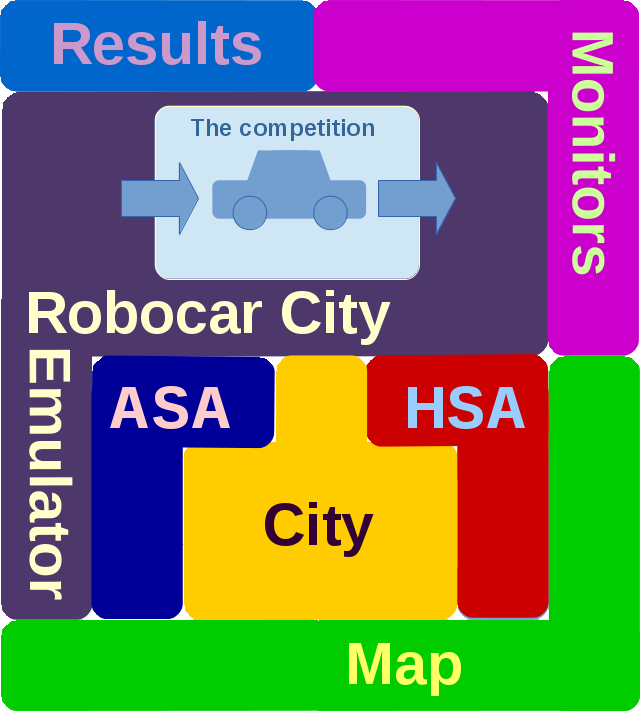
\includegraphics[scale=.3]{img/tetris_plan.png}
\caption{This figure shows the tetris plan of the OOCWC system. The overlapping components have a connection with each other. Source: \cite{infocomjournal}.}
\label{tetris_plan}
\end{figure}

\subsection{The Map and the City}
\label{map}

In the past few years, numerous map databases have become available for public. These databases can be used for route planning, location discovery and POI search. One example is Google Maps, with which we can navigate on smartphones, plan routes on other devices and have a rich POI database. Another example is Microsoft Bing Maps. In general, these two databases use data from multiple sources created with professional tools. Using these maps are free for private use only.

In contrast, the OpenStreetMap (OSM) is a database that was created and is being developed by a community of volunteers. OSM is free for both private and commercial use. In paper \cite{openmapsimul}, we investigated the usability of OSM in the OOCWC system. The main question was: is a free, community-based map database accurate enough to use for professional purposes?

Since the OOCWC platform has a GNU GPL version 3\footnote{\url{https://www.gnu.org/licenses/gpl-3.0.en.html}} software license and is free to use and develop as an open source software, the license of OSM (Open Data Commons Open Database License\footnote{\url{https://opendatacommons.org/licenses/odbl/}}) is suitable for our purposes. In the selection of the map database, one important factor was the license. We needed an open and free database, but we did not want to use a database that has a copyleft license. Therefore, we have the opportunity to close the source of the OOCWC system for commercial use.

Data from the OSM can be downloaded\footnote{Debrecen: \url{https://www.openstreetmap.org/export#map=13/47.5302/21.6469}} in XML format. The XML file consists of real-world objects.\footnote{\url{https://wiki.openstreetmap.org/wiki/Map_Features}} These objects can be nodes, ways and relations. Every object can have a tag that connects it to its real-world pair. Every object has an ID and coordinates in the WGS 84 geodetic system (\enquote{GPS coordinates}). A node can be an individual object (e.g. a building) or it can be a point on a way or a street. Relations define connection between ways and nodes (e.g. bus lanes), but these relations are not used in the OOCWC currently. Source \ref{osm_xml_example} shows part of an OSM XML file, a way (Gyöngyösi street, Debrecen) and a node on that way.

\begin{lstlisting}[language=XML,caption=Short example of OSM XML with a way in Debrecen (Gyöngyösi street) and a node on that way., label=osm_xml_example]
<way id="24595720" version="7" timestamp="2011-08-16T09:49:58Z" changeset="9033539" uid="247611" user="SzPaula">
    <nd ref="249781713"/>
    <nd ref="1369686846"/>
    <nd ref="1369686858"/>
    <nd ref="1369672817"/>
    <nd ref="267375701"/>
    <nd ref="267375702"/>
    <nd ref="277120104"/>
    <nd ref="267375703"/>
    <nd ref="267375698"/>
    <tag k="highway" v="residential"/>
    <tag k="name" v="Gyongyosi utca"/>
  </way>

<node id="1369686846" lat="47.5448353" lon="21.6186001" version="1" timestamp="2011-07-22T06:58:20Z" changeset="8794632" uid="493626" user="tamaas"/>
\end{lstlisting}

In the OOCWC system, we process the XML file with the Osmium software library as follows. We process every way tagged as \textit{highway} which is accessible by car. Therefore, tags with the \textit{footway}, \textit{cycleway}, \textit{bridleway}, \textit{step}, \textit{path}, \textit{construction} values are not important. We also leave out traffic lights and other signs. From the data, the software creates an adjacency list for every node. This adjacency list consists of key-value pairs, where the key is an OSM node ID, and the value is a list of node IDs of the adjacent nodes of the corresponding node. This adjacency list defines a directed graph (which will be described in chapter \ref{simul}). In addition, we also store the Haversine distance\footnote{\url{https://docs.osmcode.org/libosmium/latest/haversine_8hpp.html}} of the adjacent nodes in a list. For route planning we use the Boost Graph Library (BGL).\footnote{\url{https://www.boost.org/doc/libs/1_66_0/libs/graph/doc/}} We build two alternative data structure, one using a directed routing graph, and another using a BGL graph. The simulation is based on the directed graph, but simulation clients may use the BGL graph as well.

For simulation, we use a rectangular part of the OSM, in most cases, we select a city. This is what we call \enquote{City Operating Area}. For example, in the case of Debrecen (see Fig.~\ref{debrecen_map}), the competition area (see section \ref{competition}) is bounded with coordinates N47.4095 to N47.652 and E21.4268 to E21.8628.

\begin{figure}[ht!]
\centering
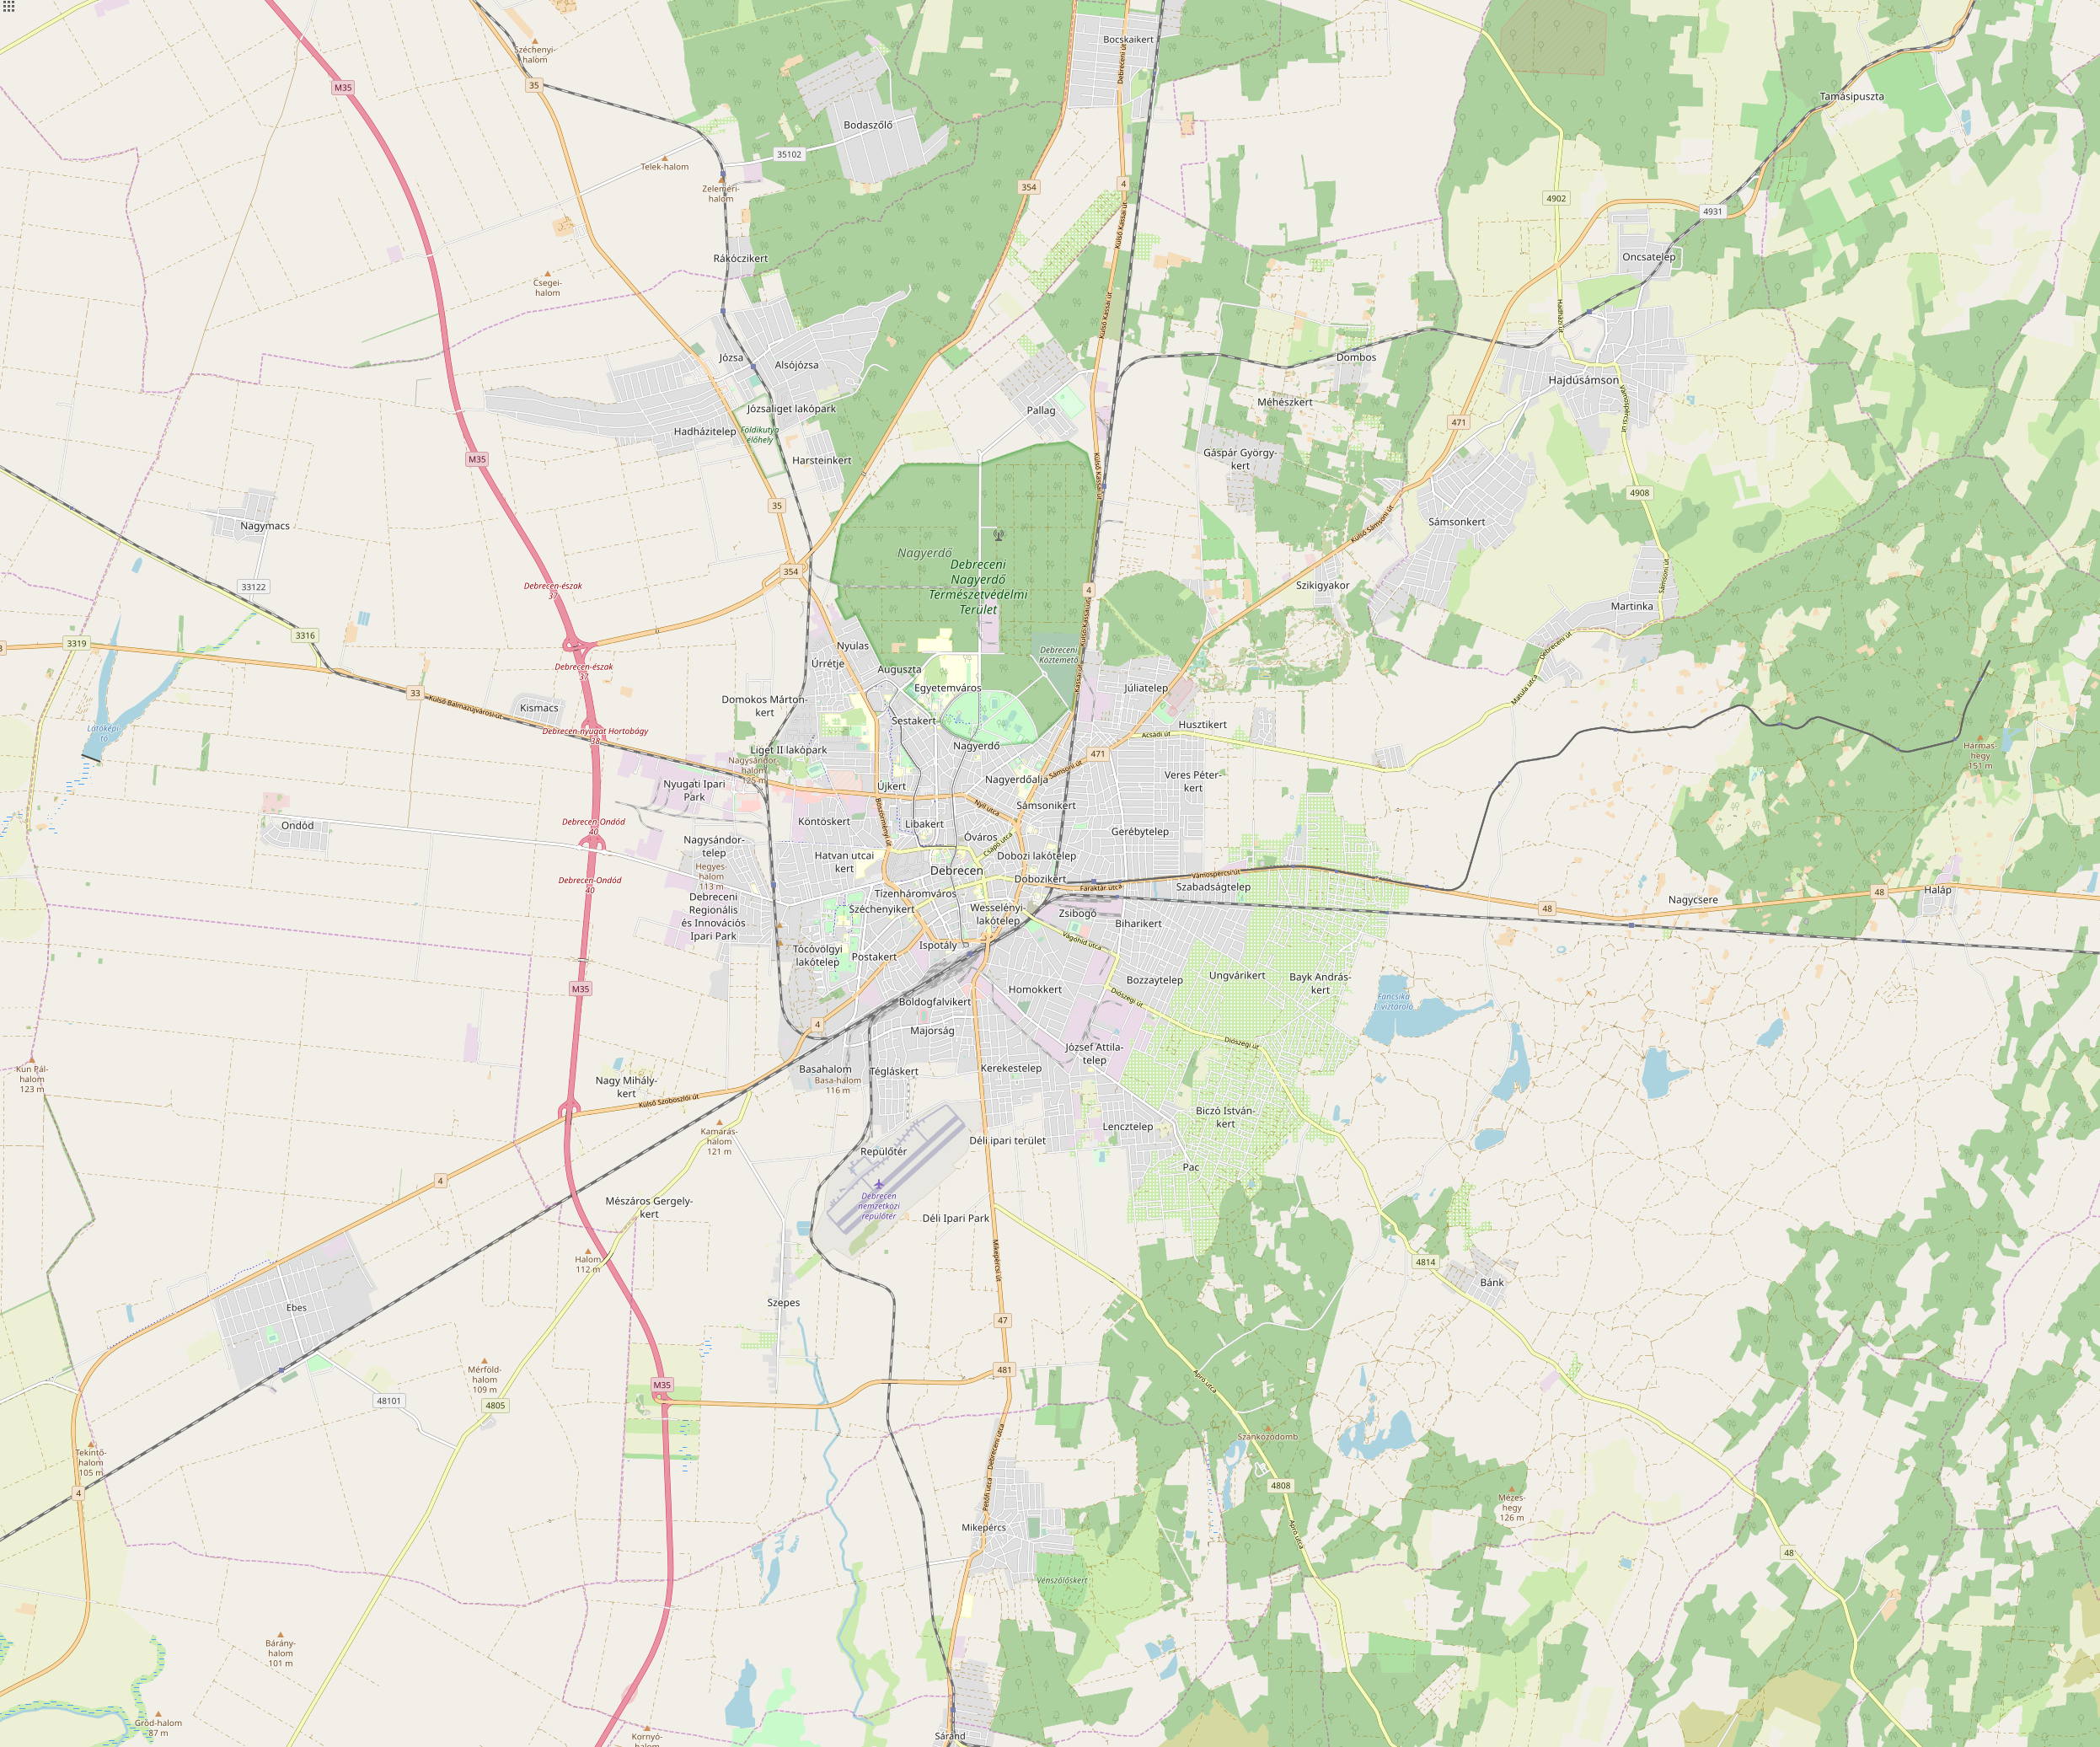
\includegraphics[width=10cm]{img/debrecen_coa.png}
\caption{The map of Debrecen exported from the OpenStreetMap database. \copyright OpenStreetMap contributors.}
\label{debrecen_map}
\end{figure}

In Fig.~\ref{dd_graph}, the graph of the downtown of Debrecen can be seen. This figure was created with the graph-tool Python library.\footnote{\url{https://graph-tool.skewed.de/}} (For more details on conversion from OSM XMLs to graphs see chapter \ref{simul})

\begin{figure}[ht!]
\centering
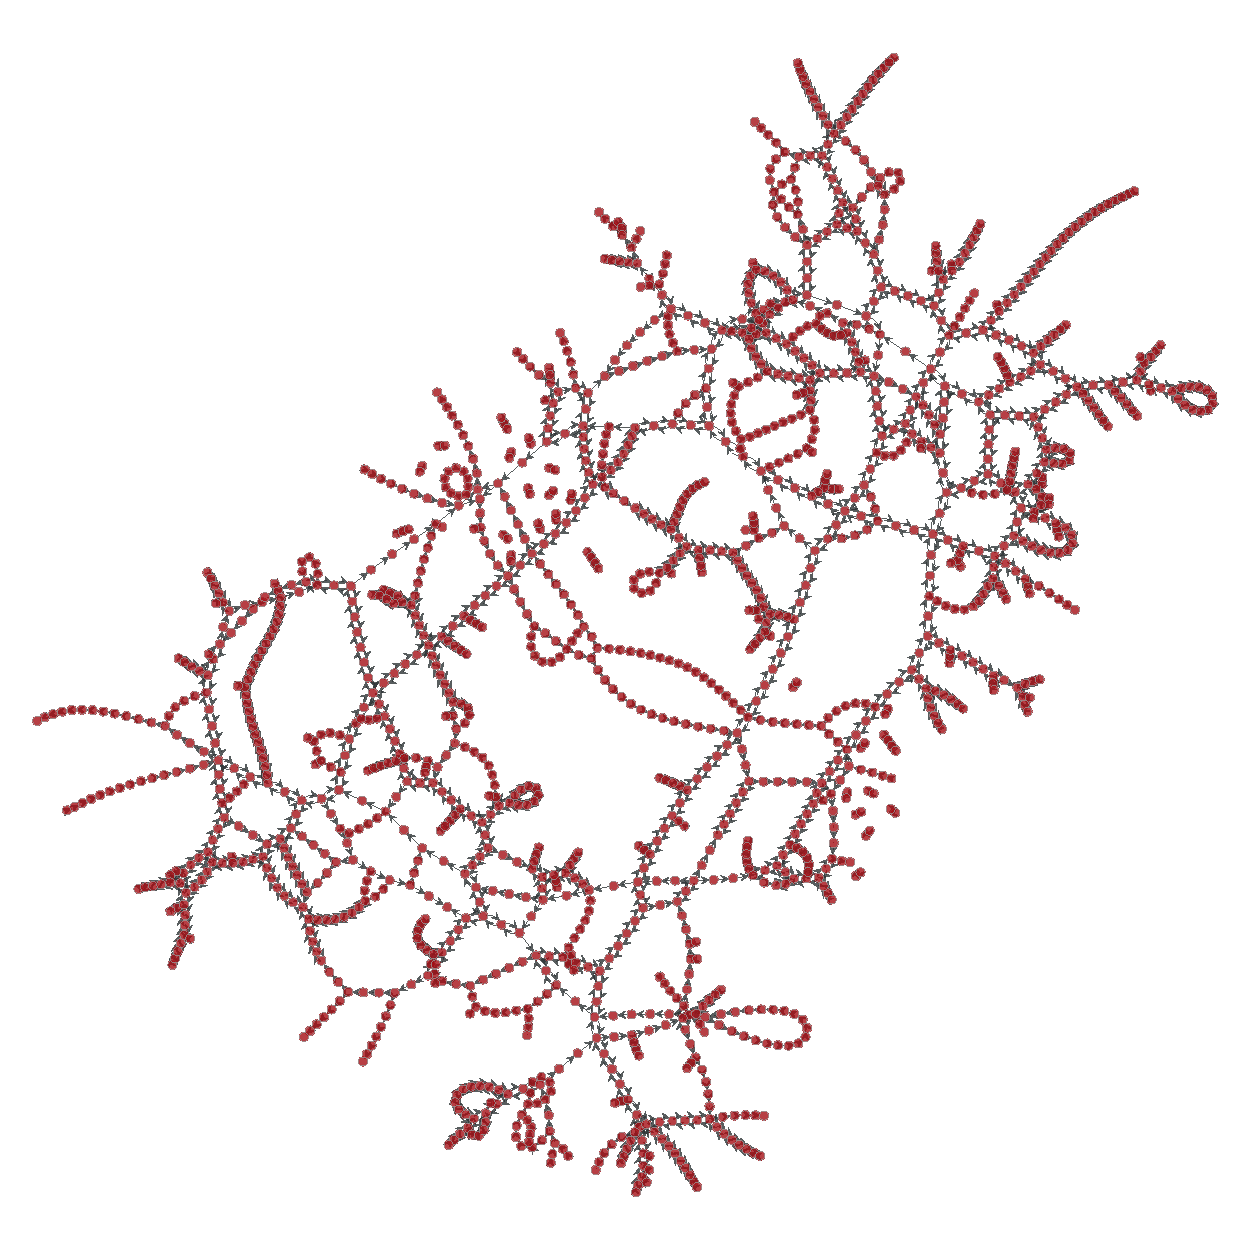
\includegraphics[width=10cm]{img/debrecen_downtown.pdf}
\caption{The graph of the downtown of Debrecen created with the graph-tool Python library.}
\label{dd_graph}
\end{figure}

\subsection{Monitors and Results}

Two monitors are included within the system, rcwin and rclog. Both have similar structure, both are based on the JXMapViewer2 library.\footnote{\url{https://github.com/msteiger/jxmapviewer2}} In Fig.~\ref{rcwin_example}, rcwin in operation can be seen.

\begin{figure}[!ht]
\begin{center}
\subfigure{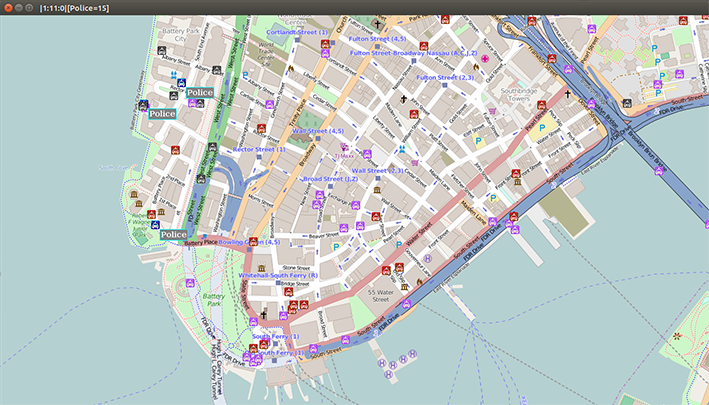
\includegraphics[width=8cm]{img/m3.png}}
\subfigure{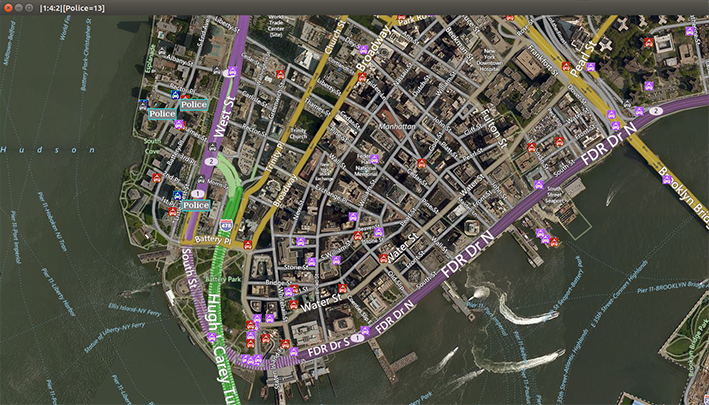
\includegraphics[width=8cm]{img/m4.png}}
\end{center}
\caption{The rcwin in operation. Source: \cite{infocomjournal}. \copyright OpenStreetMap contributors}
\label{rcwin_example}
\end{figure} 

\subsection{The competition aspect}
\label{competition}

The original main edition of the OOCWC is called the \enquote{Police Edition}. The primary aim of this edition is to facilitate research and development of the OOCWC system, simulation algorithms and routing algorithms. We organized competitions around the system, hoping that better and better solutions could arise. A similar approach can be found in other research domains, such as artificial intelligence, where the RoboCup initiative \cite{kitano1997robocup} organizes competitions for the development of agent-based AI algorithms. In the OOCWC system, three different types of agent exist in the simulation, routine cars, smart cars and guided cars (for more, see section \ref{rcemu}). The aim of the competition is to catch as many gangster agents (smart cars) as possible with 10 police agents (guided cars) in 10 minutes. Competing teams control the police agents. Since in the OOCWC system all cars are multi-agent based entities, every car of a given type has the same controlling algorithm and heuristics (e.g., the closest gangster is pursued).

Paper \cite{forkcoginfocom} describes our solution.\footnote{A demonstration video can be found at \url{https://youtu.be/MzH-0i4VGMk}.} In this implementation, one cop pursues one gangster. We set cop-gangster pairs based on distance: every cop pursues the closest gangster. First, we used Haversine distance, which gives the distance between two points on a sphere given their latitudes and longitudes, but it did not show satisfying results. Then, we implemented a different solution that takes into consideration the length of the roads and the one-way streets. The basic algorithm in the OOCWC can handle only one cop at a time. The method implemented by us can handle $N$ distance. This gives us a $N\times M$ matrix which contains all cop--gangster distances. (These distances are not symmetrical, because of one-way streets.) In this matrix, we search for the smallest value ($M_1$, $N_1$) that will be the best pair, so the $M_1$ cop will pursue the $N_1$ gangster. The code snippet in Source \ref{police_example} shows this implementation.

\begin{lstlisting}[language=C++,caption=Code snippet of the algortihm created for the Police Edition., label=police_example]
//Calculate the Cop_gangster matrix
for (int i = 0; i < 10; i++){
    
    int *dists = dijkDist(w_cops[i].to, w_gangsters);
    
    for (int j = 0; j < number_of_gangster; j++){
        m_cop_gangster[i][j] = dists[j];
    }
}
int it = 10;
//Sort the matrix
while (it-- > 0){
    int MAX = 10000000;
    int min = MAX;
    int i_cop = -1;
    int j_gang = -1;
    
    for (int i = 0; i < 10; i++){
        for (int j = 0; j < number_of_gangster; j++){
            if (m_cop_gangster[i][j] < min){
                min = m_cop_gangster[i][j];
                i_cop = i;
                j_gang = j;
            }
        }
    }
    //....//
}
//Routing
for (int i = 0; i < 10; i++){
    Cop  c = w_cops[i];
    Gangster g = gcop[i];
    Dijkstra target = dijkstraAll(c.to, g.to);
    route ( socket, c.id, target.path );
}
\end{lstlisting}

About the performance of this algorithm, we can state that on an Apple MacBook Air 11" (Model A1465) laptop (Intel Core i5 1.4 GHz CPU, 2 core, 4 thread, 4 GB RAM) calculating the matrix (i.e.~100$\times$10 routes) took about 200 milliseconds on the map of Debrecen (the matrix consists of 77,591 edges and 37,455 vertices).

\subsection{Robocar City Emulator}
\label{rcemu}

The main component of the OOCWC system is the Robocar City Emulator (RCE). This component has several tasks:
\begin{itemize}
\item The Smart City Server opens the map database, converts it into a BGL graph.
\item The Traffic Server simulates the traffic.
\item Simulation agents (e.g., clients) can connect to the server and operate.
\end{itemize}

There exist several approaches for traffic simulation. Realistic traffic simulations have already been used in \cite{realsim}. The traffic simulation model of the RCE is based on the Nagel-Schreckenberg (NaSch) model \cite{nasch}, because it uses a cell-based approach, as well. Three classes of traffic simulation models exist: 

\begin{enumerate}
  \item Agent-based models (or microscopic models), for example, see \cite{treiber2000congested}, \cite{duncan1997high}.
  \item Continuum models (or macroscopic models), for example, see \cite{fan2013comparative}, \cite{sewall2010continuum}, \cite{chrobok2001traffic}.
  \item Hybrid models, for example, see \cite{sewall2011interactive}.
\end{enumerate}

The RCE uses the agent-based approach, moreover, it can be considered as a standalone multi-agent system. For more on traffic simulation see section \ref{simul}.

The first rapid prototype of the OOCWC system is called Justine. It has 3 main components, the RCE, the rcwin and the rclog. This prototype uses the OSM database and processes it with the Osmium Library. The result of this processing is a routing map graph and a BGL graph. The routing map graph then placed into a shared memory segment by the smart city server. The traffic server simulates the traffic. A sample client program is provided to the original version that demonstrates how a client can connect to the server and how the shared memory segment should be operated. One implementation of the RCE is the \enquote{Police Edition}.

\paragraph{Basic operation of the simulation model}
As we mentioned earlier, the simulation takes place on a rectangular part of the OSM. In the case of the standard competition map of Debrecen, the routing graph has 77,591 edges and 37,455 vertices. We slice all edges for parts 3 meters long. Based on NaSch terminology, these parts are called cells. Therefore, the cell length is equal to 3 meters. Since one simulation step lasts for 200 milliseconds, all cars move with the same velocity, 54 kmh. Edges can contain a given number of cars only (calculated as the edge length divided by the length of the cell, or part, i.e.~3 meters), since one cell can contain only one car. For simplicity, we use only one lane per direction for a road segment.

In the original implementation, the traffic server moves the cars by random walk or ant simulation \cite{ant1}, \cite{ant2}. In the case of RCE, random walk means that when a car arrives at an intersection (i.e.~graph vertex) it choses its next street (i.e.~graph edge) based on uniform distribution. Ant simulation means that the next edge is selected with a probability that increases based on previous selections. In addition, the sample client has an implementation of Dijkstra's and Bellman-Ford algorithms (using the BGL) \cite{siek2002boost}.

One of the biggest challenges during the development was to find a solution that can handle a large number of cars. Obviously, we could not implement cars as individual UNIX processes or Java/CUDA threads. No current operating system can handle this amount of individual process. So, a routine car only has a probability distribution on the map. The initial distribution of the cars can be measured or estimated. Then, all cars move according to the aforementioned ant simulation or random walk. In chapter \ref{simul}, we show that this simulation approach is not accurate enough and introduce a mathematically rigorous stochastic model called \enquote{Markov traffic}.

\chapter{Data collection -- The Real-Time Traffic Analyzer}
\label{rtta-chapter}

Most smart city applications depend not only on well-designed ICT infrastructure but real-time data. In most cases, these data are collected with some sort of ICT device, but it can be a viable option to involve inhabitants in data collection. On the tetris plan of the OOCWC system in Fig.~\ref{tetris_plan} the ASA (Automatic Sensor Annotations) and HSA (Human-controlled Sensor Annotations) components are considered to implement these corresponding approaches. For data collection in smart cities, we outline a framework in paper \cite{szabo2013framework}. 

The framework is an outline of smart city applications that are based on participatory sensing; this approach involves inhabitants in the data collection actively. With the widespread use of smartphones, more and more computational capacity and sensors are available in the hand of inhabitants. If a community finds an application useful, they will participate in its operation. This context sharing (or crowdsourcing) combined with big data analytics can realize the Internet of Things (see Fig.~\ref{framework_iot}). One good example can be the Waze navigation system, where users can annotate certain events of traffic (e.g.~accidents, detours, etc). More examples can be seen in paper \cite[chapter III]{szabo2013framework} and \cite{besenczi2013kozossegi}. Although this framework is developed especially for participatory sensing, crowd-sensing based applications can work following the presented approach.

\begin{figure}[ht!]
\centerline{
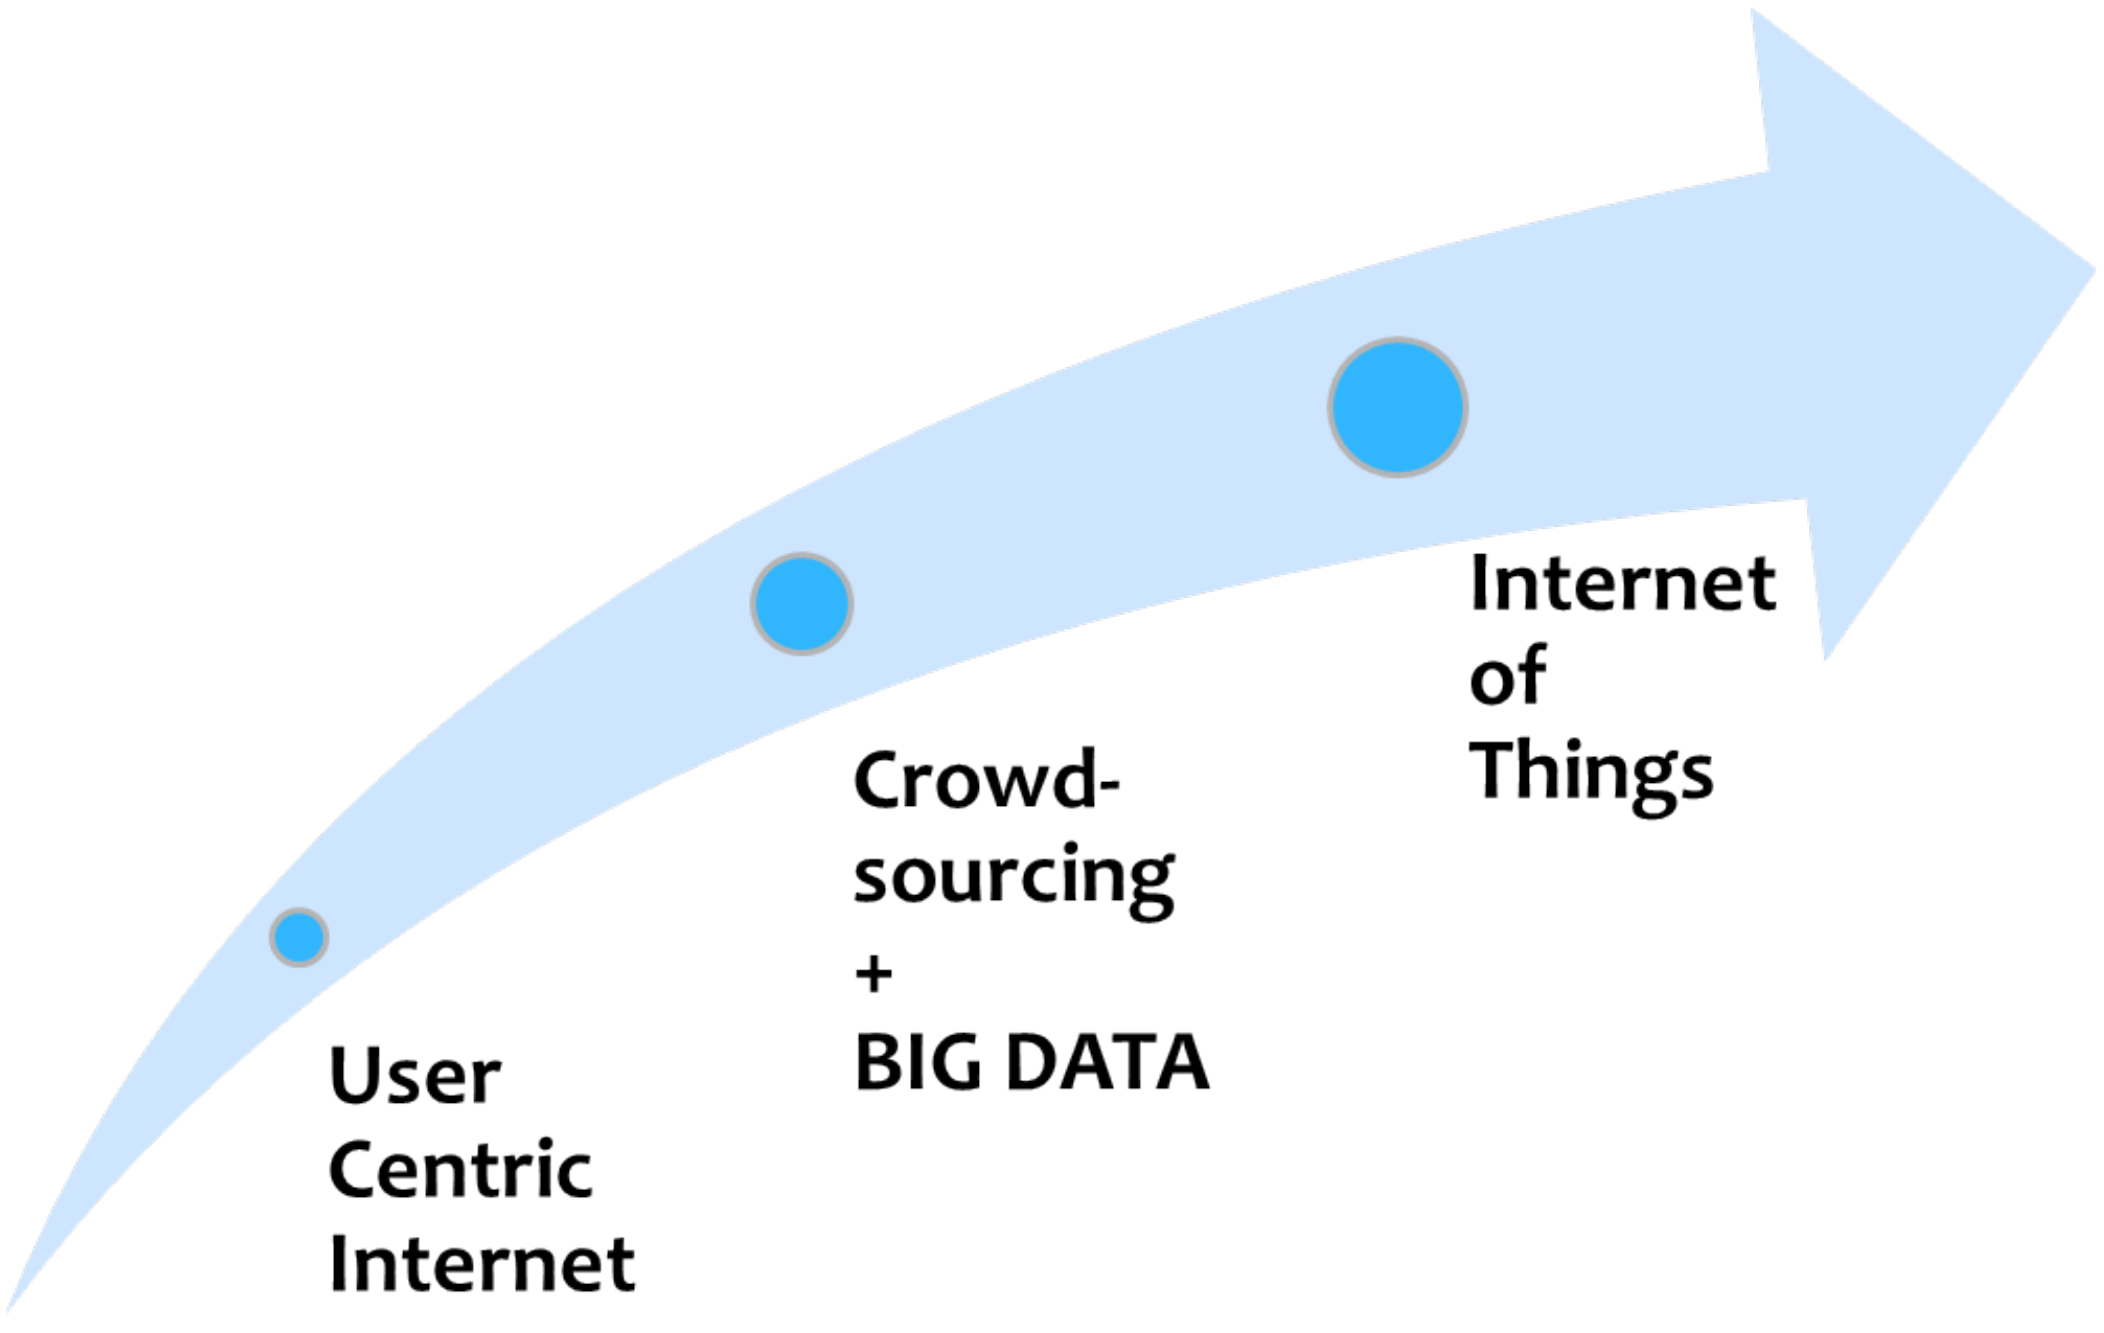
\includegraphics[width=8cm]{img/framework_iot.png}}
\caption{Internet evolution in our vision. Source: \cite{szabo2013framework}.}
\label{framework_iot}
\end{figure}

An average crowd-sourcing application nowadays consists of two components, one at the user's device and another one in the cloud \cite{ganti2011mobile}. This may result in unnecessary developments and slow innovation and development cycle. In our framework, we separate application logics from analytics and communication. To provide development that is independent from other components, the framework must pass extra information, by which its services can be extended. For this, we need an approach based on some sort of extensible messaging service. In addition, in the case of participatory sensing, we must separate information producers and consumers in time, space and synchronization.

Because of the lack of a framework that separates producers from consumers, we proposed a system for participatory sensing based smart city applications. The system (Fig.~\ref{framework_layers}) consists of

\begin{itemize}
\item a communication framework (including an advanced messaging protocol);
\item analytics;
\item applications.
\end{itemize}

\begin{figure}[ht!]
\centerline{
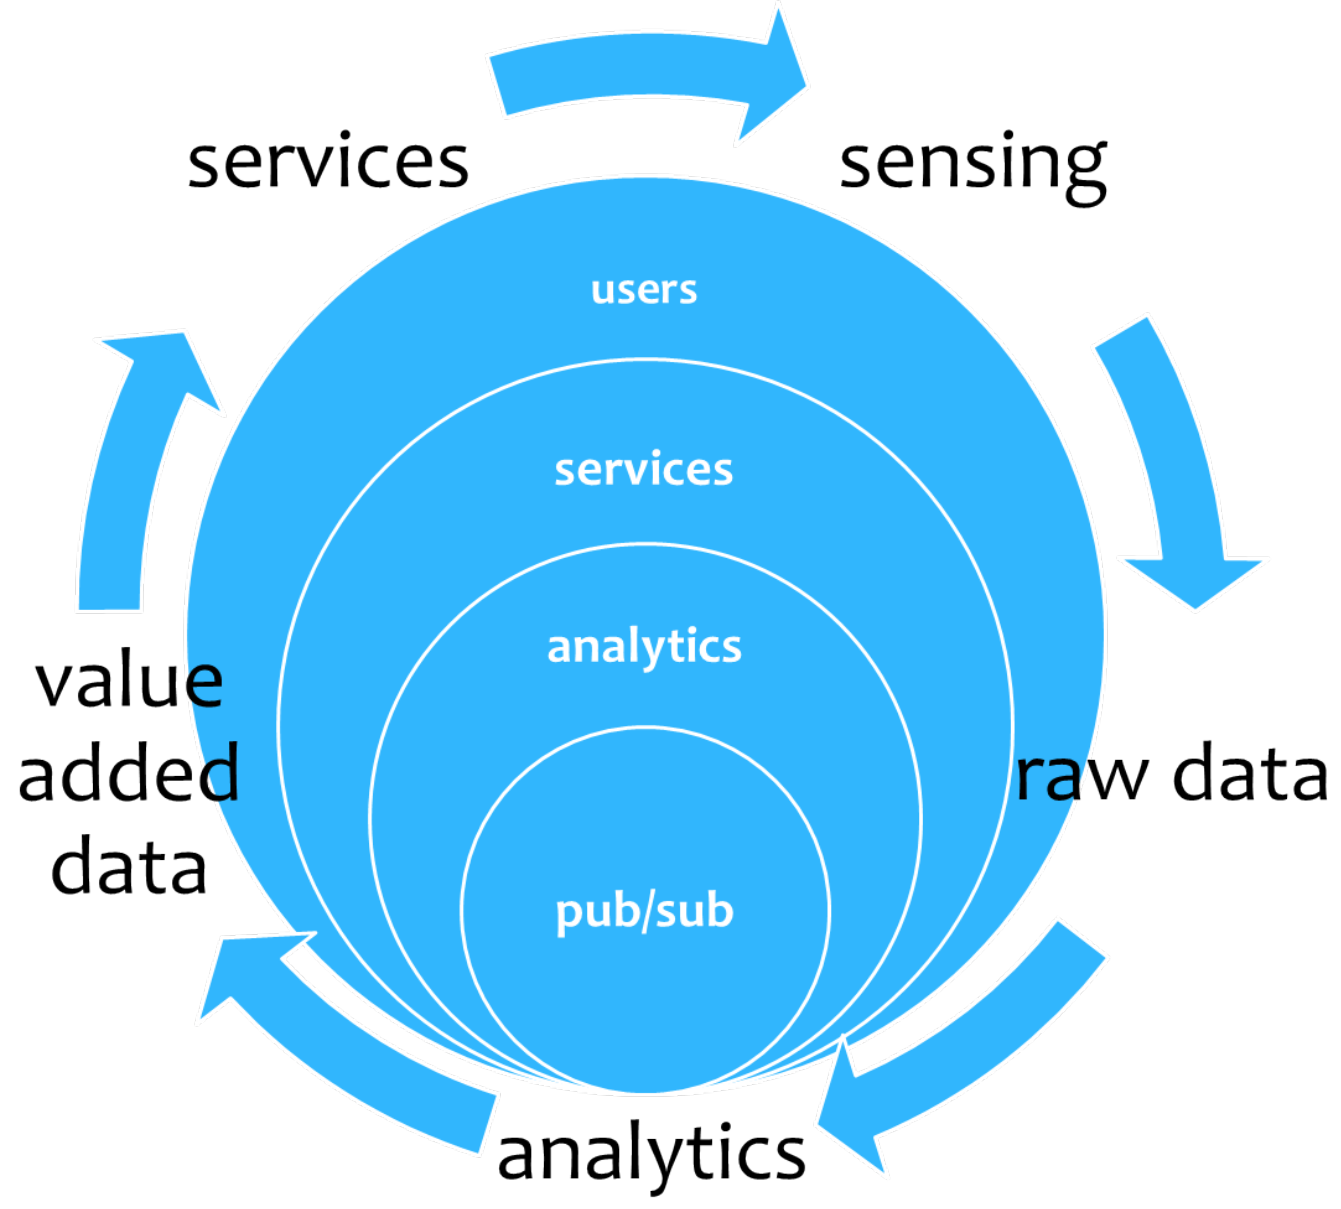
\includegraphics[width=6cm]{img/framework_layers.png}}
\caption{Production chain from sensing to services. Source: \cite{szabo2013framework}.}
\label{framework_layers}
\end{figure}

In the framework, we originally investigated the Extensible Messaging and Presence Protocol \cite{saint2011extensible} because of its publish-subscribe (pubsub) \cite{millard2010xep} service. The communication scheme of crowd-sourcing based applications is somewhat similar to the basic scheme of pubsub. Users collect data (or \textit{publish} their data), and use services offered by the system (or they \textit{subscribe} to services). Therefore, in this model, we define three roles: \textit{Producers}, \textit{Service Providers} and \textit{Consumers} (see Fig.~\ref{framework_roles}). Every entity interacts via pubsub nodes, which are event based.

Producers are the original information sources; they are users who collect data. Consumers are using the data provided. In some cases, they can act as Producers as well. Service Providers analyze, aggregate, and add value to the raw data.

In the model shown on Fig.~\ref{framework_roles}, Producers publish (depicted with empty arrowheads) the collected (raw) data to pubsub nodes (depicted with blue circles). Service providers subscribe (shown as filled arrowheads) to these nodes and publish their value-added information to other pubsub nodes (depicted with orange circles). Consumers (who can be Producers as well) subscribe to these nodes, so they can obtain this value-added information. An important property of this pubsub approach is that the information flow occurs asynchronously.

\begin{figure}[ht!]
\centerline{
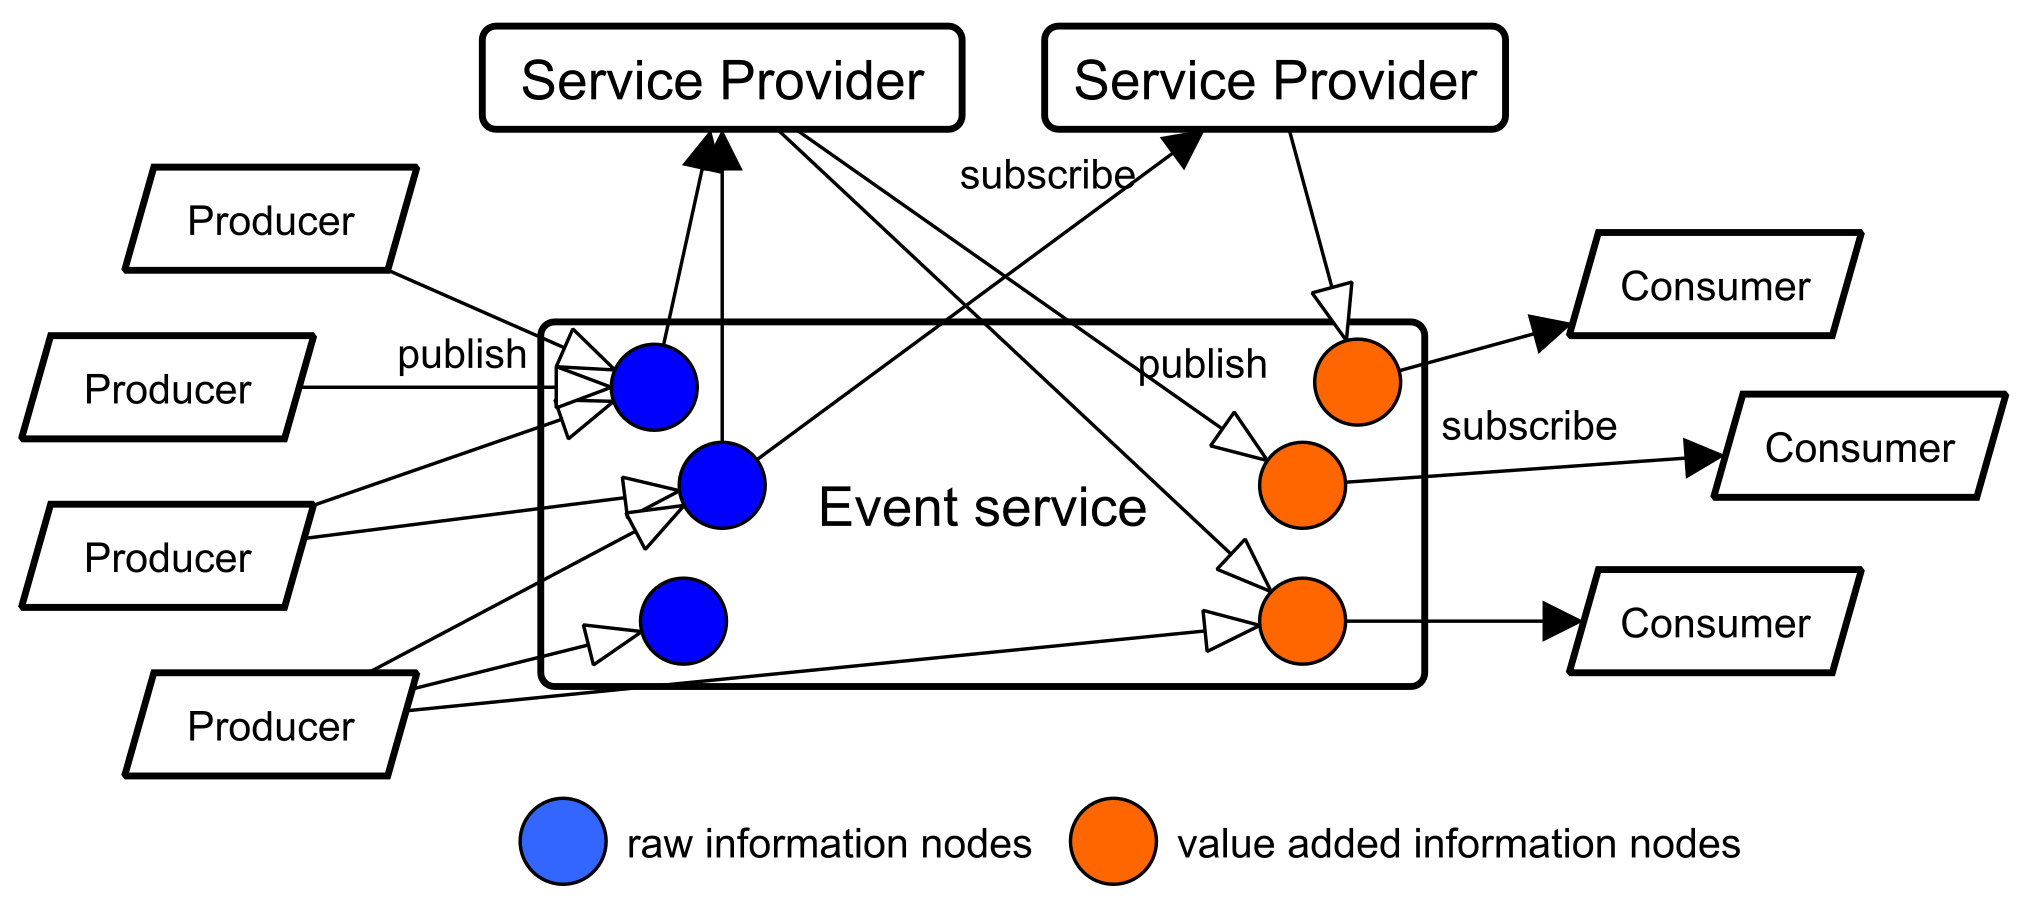
\includegraphics[width=12.6cm]{img/framework_roles.png}}
\caption{Roles and their interaction in the pubsub architecture. Source: \cite{szabo2013framework}.}
\label{framework_roles}
\end{figure}

The publish-subscribe architecture (originally introduced in XMPP) can directly map our communication scheme (see Fig.~\ref{framework_scheme}). Raw data nodes and value-added information nodes (or service nodes) are created by Service Providers. Producers and Consumers with appropriate node rights can publish their collected data to raw data nodes, and only the owner of the node can pull data from these nodes with the subscription service. Service providers publish information to the service nodes. Consumers subscribe to these service nodes and may retrieve value added information. In most cases, consumers can decide which node they subscribe to, so they get appropriate information. XMPP has a data aggregation feature, but we should note that this feature cannot filter events. On Fig.~\ref{framework_scheme}, this aggregation is denoted as dark circles, whilst empty circles indicate aggregation that is implemented as a service logic.

\begin{figure}[ht!]
\centerline{
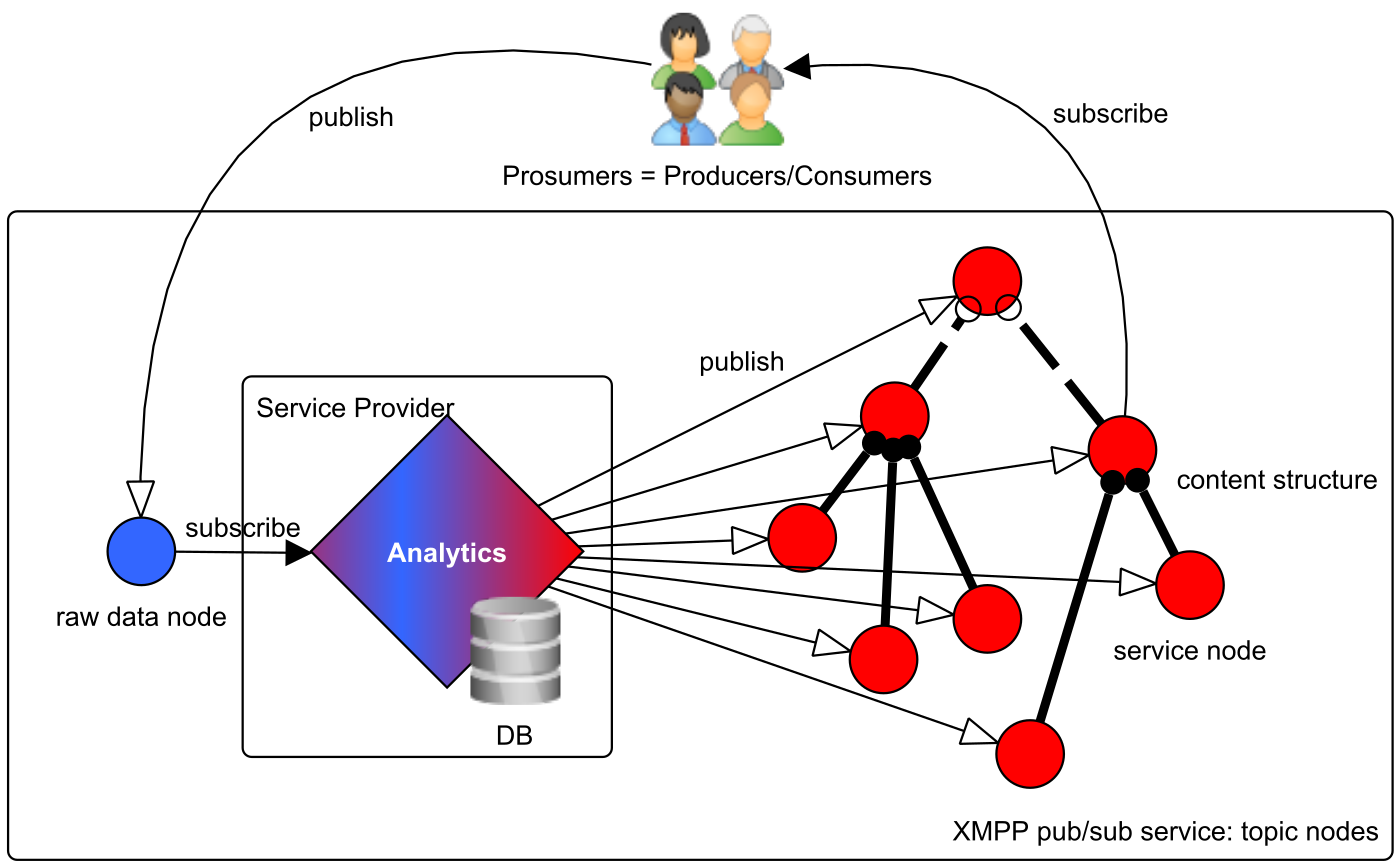
\includegraphics[width=12.6cm]{img/framework_scheme.png}}
\caption{Participatory sensing information chain. Source: \cite{szabo2013framework}.}
\label{framework_scheme}
\end{figure}

To briefly summarize, crowd-sensing and crowdsourcing (and participatory sensing) are tools with which we can measure certain conditions in a city and we can obtain information about citizens and their environment. The inspection occurs on an individual level and we investigate data on an aggregated level (crowd level).

The input of the RCE will be stored in the Robocar City Cloud. (The cloud service is not available yet.) This cloud will perform data aggregation, analysis, and will store the dataset of the city where RCE operates (can be considered as an analytics tool shown on Fig.~\ref{framework_scheme} that subscribes to the raw data nodes). As we mentioned earlier, two types of data collection approach exist. First, a community-based data collection, called participatory sensing or crowd sourcing, where the user's (or crowd's) active \textit{participation} is required. In the scheme of the OOCWC this component is the HSA. We will develop mobile phone applications that have a simple GUI, like in \cite{besenczi2013kozossegi}. One use case is when an individual traffic unit measurement occurs with the tap of a soft-key of the application. In the sense of the above-mentioned smart city framework, this role is the \textit{Producers}. This functionality is not yet implemented.

The other data collection type is crowd-sensing. In the scheme of the OOCWC system, this is the ASA component. The devices, developed by us, are collecting data without human interaction. This component is considered as a \textit{Producer}, as well. As a first step of development, we outlined the requirements of this system. The main points are the following:

\begin{itemize}
\item Real-time operation, local image processing.
\item Real-time connection with a cloud-based service.
\item Accurate positioning.
\item Ease of assembly into cars.
\end{itemize}

We imagined the development in three different directions. The main difference is the type of the CPU. We apply a Field Programmable Gate Array (FGPA) in every solution, and all peripherals are the same. As input devices, we use an image sensor and a GPS (Glonass) module; as an output we use a standard GSM module. We conduct the development on \enquote{development boards}. The three directions are as follows.

{\bf{ARM based solution.}} The fast processing property of the FPGA is used for the I/O subsystem and the memory. The ARM provides a standard platform for calculations, and for image processing. The main advantage of this type is that we can use an Embedded Linux System (ELS), so the high-level processes can be implemented in a standard Linux environment. One such ARM based system is the Raspberry Pi single-board computer (but without FPGA).

{\bf{Soft-processor based solution.}} In this type there is no physical, dedicated CPU, but we can add one for the hardware design (e.g.~a Xilinx MicroBlaze). In this case, we can define the operation of the CPU, but its instruction set can be a limiting factor. Using an ELS, like the case of ARM based solutions, is possible.

{\bf{Raw FPGA design.}} In this case, there is no CPU at all. The I/O system, the memory and the image processing methods are all implemented in the FPGA; technically, it is a pure hardware design. Regarding the computational capacity and execution times, this is the best solution, but its development cycle is longer.

As a conclusion, we can say that the ARM based solutions are more flexible and easier to extend with new functionality, but we are limited to the properties of the ARM (clock frequency and instruction set). Because development boards based on ARM are relatively cheap and easy to access, and the development cycle is shorter, one can build a development community around a project easier. Raw FPGA designs provide faster processing but their development cycle is longer and complicated (i.e.~more expensive). In the current state of the project, a prototype of the ARM based solution is provided. We will describe this prototype in this section.

\section{Technology overview}

In the first phase of development, we implemented the data collection system to an ARM based hardware. For this, we needed a device that provides flexibility during development. For example, the Raspberry Pi single-board computer (its first edition) was not suitable, because of its limited computational capacity and poor periphery handling. (The recent versions of Raspberry Pi are more suitable, and the system could be implemented on them.) Since ARM is a ubiquitous CPU type, compilers are available, and we can use an ELS, as well. We chose to use the Zynq System-on-chip (SoC).

In this section, we describe in detail the hardware and software components of the data collector subsystem.

\subsection{Hardware}
\label{rttahw}

The scheme of the system can be seen in Fig.~\ref{rttaschema}, and the detailed scheme is shown in Fig.~\ref{detailedscheme}.

\begin{figure}[ht]
\centerline{
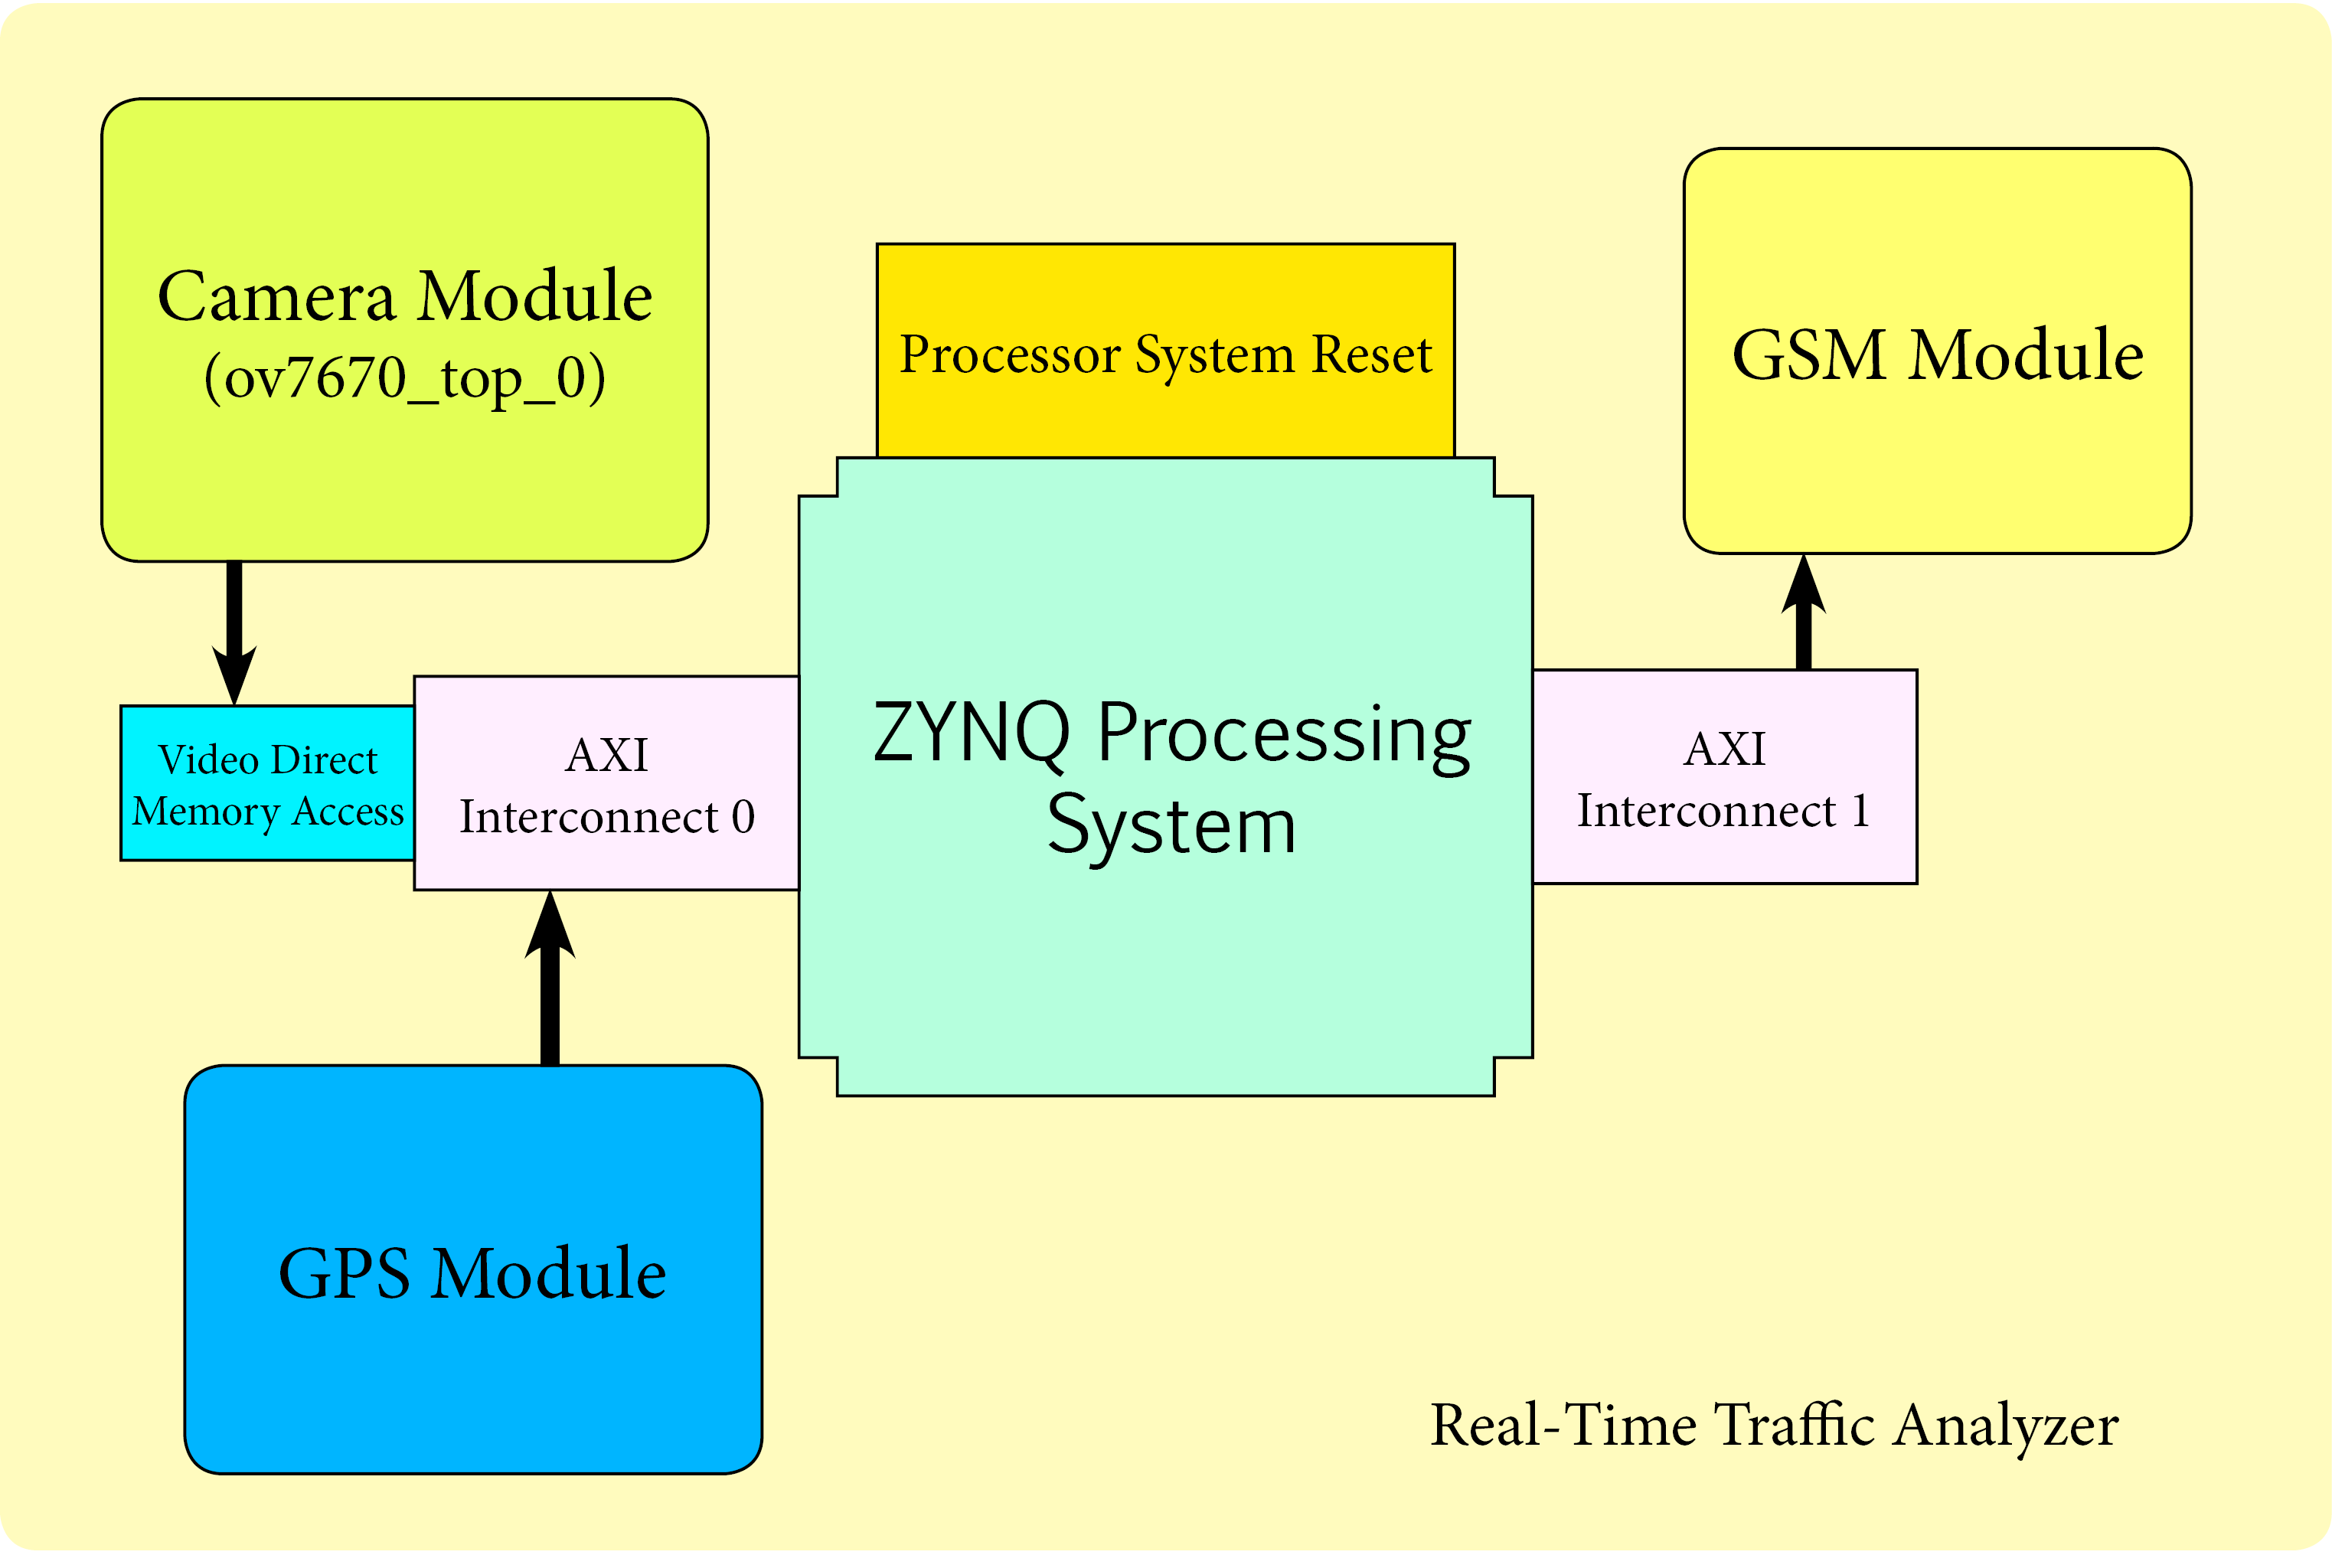
\includegraphics[width=12cm]{img/sema.png}}
\caption{The scheme of RTTA. Source: \cite{usingcoginfocom}.}
\label{rttaschema}
\end{figure}  

We developed the system on a Digilent Zybo development board\footnote{\url{http://www.digilentinc.com/zybo/}}. As shown in Fig.~\ref{detailedscheme}, the central component of the system is the Zynq Processing System, with the Processor System Reset. The devices are connected through the standard Advanced Extensible Interface (or AXI for short, \cite{xilinx1999reference}) bus protocol. 

The two main components are the two UartLite serial ports. The communication with the GPS module is provided through the \emph{axi\_uartlite\_0} serial port with 4800 baud (1 PPS data). (The GPS sends measurable data once per second.) The connection with the GSM module is provided through the \emph{axi\_uartlite\_1} serial port with 115,200 baud. 

The \emph{ov7670\_top\_0} reads data from the camera module and converts it into AXI compatible stream. The \emph{axi\_vdma\_0} module loads camera data into the memory via the \emph{axi\_interconnect\_0} module. 

The communication between the peripheries occur via the AXI bus, which has a 100 MHz base clock frequency. For sending camera data, we use a 150 MHz secondary clock.

Video Direct Memory Access (VDMA) provides a high-speed connection between the memory and the camera module. We load the video stream into memory with the resolution of 640$\times$480 pixel. The VDMA is relatively easy to use, and thanks to its Linux driver, we can easily integrate it into the system.

For our aims, the Vincotech A1080-A GPS module seems suitable. It requires minimal external components and communicates through serial port. The module sends data 1 PPS which is processed by our application on the Linux system (see the next section). The time and the actual position are both important to us. We should note that the power provided by the Peripheral Module (PMOD) is enough for this module.

For internet connection, we use a SIM900 GSM module. Since this module requires a 5V voltage, we connected it to the Zybo board's external power supply. Because the initial peak in this type on connections can cause problems, we should pay attention for this in the future.

\begin{sidewaysfigure}
    \centering
    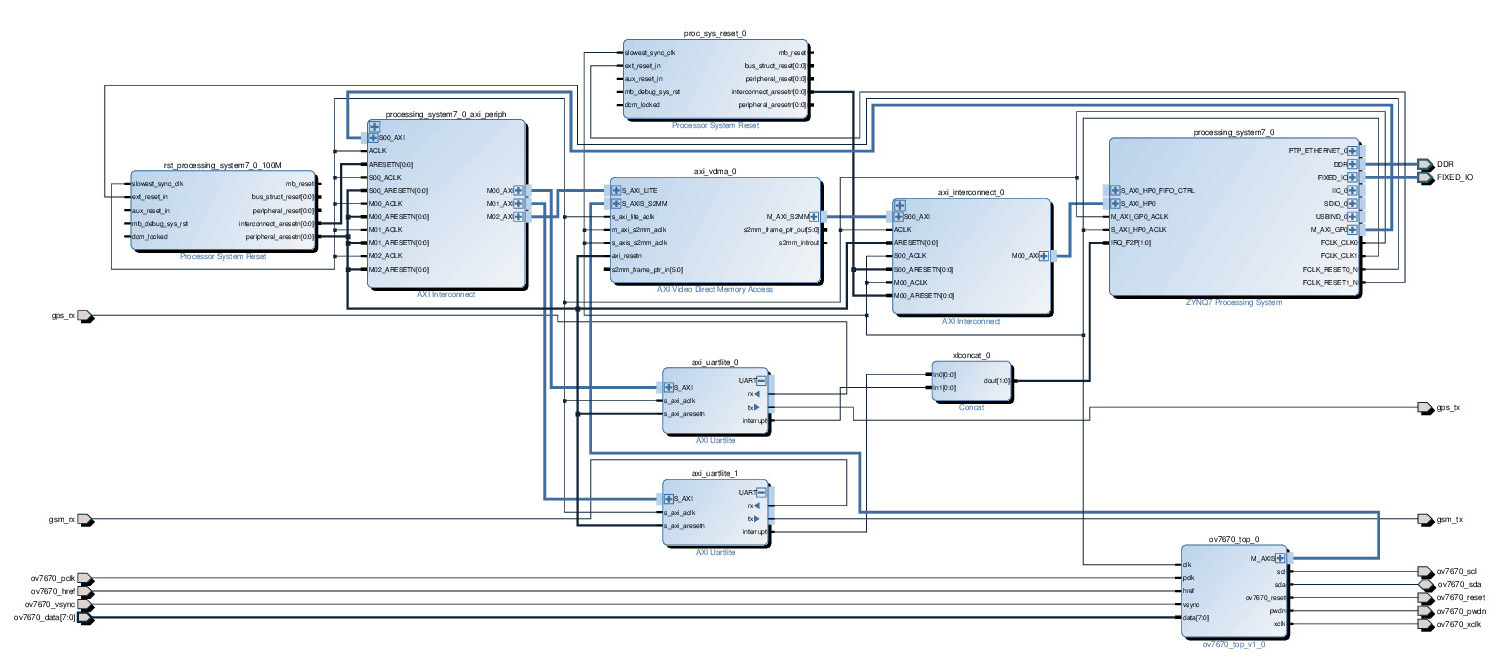
\includegraphics[width=17cm]{img/base_design_1.jpg}
    \caption{The detailed scheme of RTTA.}
    \label{detailedscheme}
\end{sidewaysfigure}

For visual perception, we use the OV7670 camera module that has a maximal resolution of 640$\times$480 pixel. One huge advantage of this unit is that we can set its resolution before operation (among several other properties). With this, we can spare some capacity of the ARM by skipping a pre-processing step of the videostream. So far, there is no FPGA supported pre-processing in the system, but we are planning to integrate a HLS based OpenCV solution.

We are planning to integrate a CAN bus communication into the system, so the device will be able to communicate with the vehicle by extracting some relevant data. The hardware parts can be seen in Fig.~\ref{currentsys}.

\begin{figure}[ht]
\centerline{
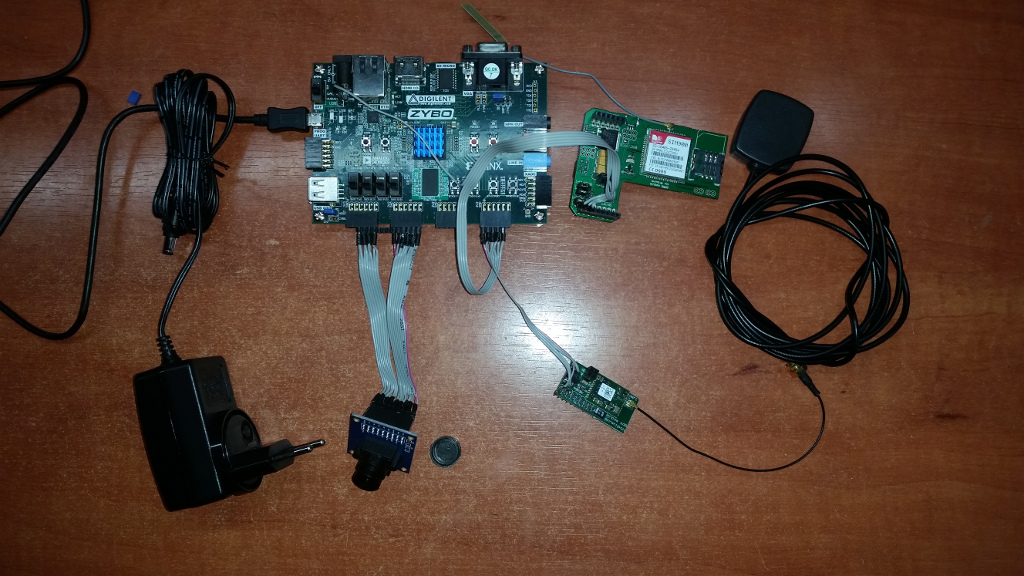
\includegraphics[width=12cm]{img/currentsys.jpg}}
\caption{The hardware parts of the system.}
\label{currentsys}
\end{figure}

We should note that the system in its current state cannot be assembled into vehicles for civilian use. During the development process, we should pay high attention for the type of the vehicle (bus, car, etc), because this will define the power supply, the case size and other limitations. The current state can be considered as a prototype, only suitable for developer testing.

\subsection{Software}
\label{rttasw}

As we mentioned before, we can run a Linux system on the ARM based development board. Linaro is an open source Ubuntu Linux based operating system, optimized for SoC systems. The software executed on the OS consists of three components:

\begin{itemize}
\item GPS component,
\item image processing component,
\item GSM component.
\end{itemize}

The program initializes the components and executes it on different threads (as shown on Source \ref{main}).

\begin{lstlisting}[language=C++,caption=Component initialization and execution., label=main]
init_gps();
MQTT_init();
init_video(argv[1]);

thread t_gps(gps_thread);
thread t_mqtt(mqtt_thread);
thread t_opencv(opencv_thread);
\end{lstlisting}

The GPS component reads the data from the GPS module and stores it in a data structure in the memory (see Source \ref{gpsstruct}).

\begin{lstlisting}[language=C++,caption=The data structure for timing and positioning., label=gpsstruct]
typedef struct GPGAA_ {
    unsigned char hour, min, sec;
    enum NS lns;
    double latitude;
    enum EW lew;
    double longitude;
    unsigned char gps_fix, sat_num;
} GPGAA;
\end{lstlisting}

For a communication protocol, we use MQTT, which is a protocol developed for \emph{machine-to-machine} communication. It has a low communication overhead and implements the publish-subscribe communication paradigm. It is a very good protocol for low bandwidth communication in low energy environments\footnote{\url{http://www.mqtt.org}}. 

The image processing method is based on a Haar-cascade classifier \cite{violacascade} \cite{haaremp}. (The source of the pre-trained cascade file: \cite{cascade}.) After initializing the videostream, we store every frame in a Mat object.

The algorithm tries to recognize a vehicle on every frame of the stream. If a vehicle recognized, a counter (\texttt{density}) is incremented with the number of recognized cars ({\texttt{object->total}}) on that frame. A car may be counted more than once if it appears on consecutive frames; this is why we call this value as \enquote{density}. We should note that if the car where the device resides stops or its speed is lower than 6 km/h for some reason (e.g.~traffic lights or traffic jam) then the calculation stops. 

It can be seen clearly that the device does not send raw image data to the server, and it performs pre-processing. We send the pre-processed data in Google Protocol Buffers format. The format of the message can be seen on Source \ref{protoobject}.

\begin{lstlisting}[language=C,caption=Protocol Buffers message format., label=protoobject]
message TrafficAnalytics{
    required string car_id = 1;
    required string timestamp = 2;
    required LatitudeNS latitudens = 3;
    required double latitude = 4;
    required longitudeEW longitudeew = 5;
    required double longitude = 6;
    required double density = 7;
    required uint32 vehicle_speed_gps = 8;
    optional uint32 vehicle_speed_can = 9;
    optional uint32 fuel_level = 10;
    enum LatitudeNS{
        NORTH = 0;
        SOUTH = 1;
    }
    enum longitudeEW{
        EAST = 0;
        WEST = 1;
    }
}
\end{lstlisting}

This pre-processing is useful from two aspects. First, in contrast with other approaches where the videostream is sent to a remote processing system, our application uses the communication channel to send only a few kBs of data every minute. The size of the videostream depends on the resolution, encoding and compression of the videostream, but it definitely requires a network connection with a much higher bandwidth. Second, data arriving from multiple sources that is evaluated and processed in a central system can cause a huge workload, thus requires a lot more computation capacity.

For the testing of the system, we developed a desktop application. The program is an MQTT broker application, to which the data collectors are connected. The input of this program is the data arriving from the devices and its output is a data structure that can be used in the OOCWC system. We describe this in detail in section \ref{cstssect}.

We should note that the system with its current operation does not cause legal (privacy) issues. In information systems that monitor civilian environment the importance of privacy is crucial. Our system does not forward or record data that have privacy related issues. The system only records and forwards the number of cars (or more precisely its density) counted in its environment. No license plate numbers, faces or any other personal data are recorded or stored.

\subsection{Development environment}
\label{dev}

Since the RTTA is a heterogeneous system, different development tools were required. The development environment of the hardware design was the Xilinx Vivado Design Suite version 2014.4. In contrast with the previously used development environments (e.g.~Xilinx ISE Design Suite), Vivado supports high level design development (but the possibility of module development remains). It supports component-based development on an advanced GUI, where projects can be assembled from modules previously developed or provided by third-party developers. We also followed this high-level development. First, we created an empty project on a Zybo board with ELS, then we added and connected each periphery. It is important to note that not every module had a predefined module description (i.e.~a \enquote{ready-to-use} module); we had to develop the GPS module.

The operating system running on the device can be added easily, we must make only a few modifications. In such, we should define the \textit{device tree}, which we should add to the Linux kernel. This device tree lists the devices and defines their I/O ports. If we define this successfully, we can use our peripheries just like in any other Linux system; as files that can be read and written. To be more precise, the data arriving from the GPS module can be read from the file assigned by the device tree in the Linux file system. Similarly, if we want to send data via GSM, we should write the file assigned to the \enquote{input port} of the GSM module. An example can be seen on Source \ref{fileops}. The first part opens the file assigned to the GPS module, the second reads it. The third block opens the file assigned to the camera module.

\begin{lstlisting}[language=C,caption=File operations in the software., label=fileops]
if ((gps_fd = open("/dev/ttyUL1", O_RDONLY | O_NOCTTY)) == -1) {
        perror("Open GPS serial: Failed to Open!");
        return -1;
    }
char read_GPS() {
    char in;
    if (read(gps_fd, &in, sizeof in) < 0) {
        perror("Failed to read GPS serial");
        exit(1);
    }
    return in;
}
if (video_fd = open("/dev/video0", O_RDWR) == -1) {
        perror("Open Video: Failed to Open!");
        return -1;
}
\end{lstlisting}

Since our software runs on a Linux system, we could conduct its development in Linux/UNIX environment. For this, we used the KDevelop IDE, the C++11 language, and POSIX threads. First, we tested our image processing methods in desktop environment, because no display is implemented in the RTTA system, so we cannot check its operation visually. The test application uses the same Haar-cascade based object detection algorithm. The operation of the program is shown in Fig.~\ref{rttapc}. On the left side, the video can be seen (recorded with an Apple iPhone 5S), with data written on it (e.g. position, date and time, timestamp, and number of cars on a given street). On the right side, we visualize the density of the traffic using the Google Maps API. In Fig.~\ref{carredrect}, the basic functionality of the object detection can be seen.

\begin{figure}[ht]
\centerline{
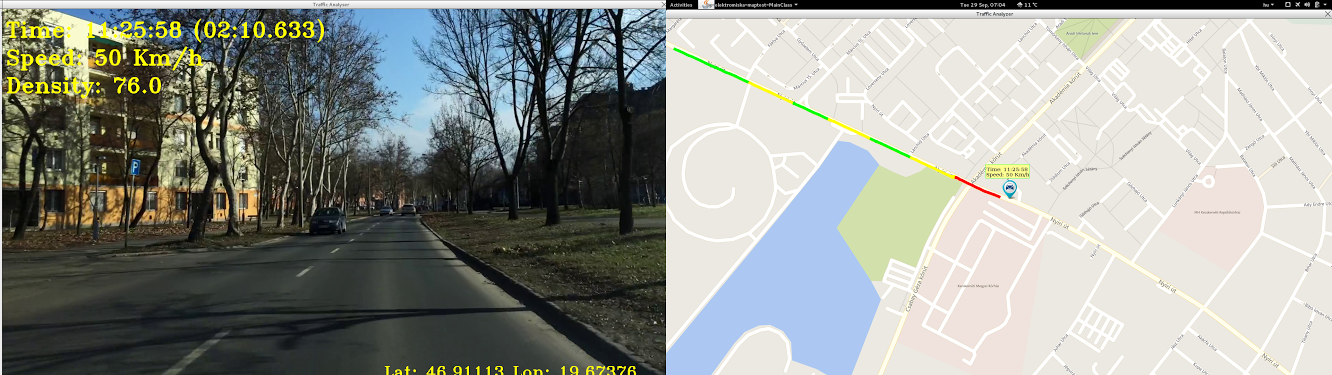
\includegraphics[width=12.6cm]{img/rttapc.png}}
\caption{Testing the image processing method in desktop environment.}
\label{rttapc}
\end{figure}

A server application is included in the RTTA system, which was developed in Java 8 in the NetBeans IDE. This app receives the data sent by the data collector devices. This program performs data aggregation using the Osmium library. In addition, the program produces a file, where every street has a vehicle density value. This file will be the input of the RCE.

\begin{figure}[ht]
\centerline{
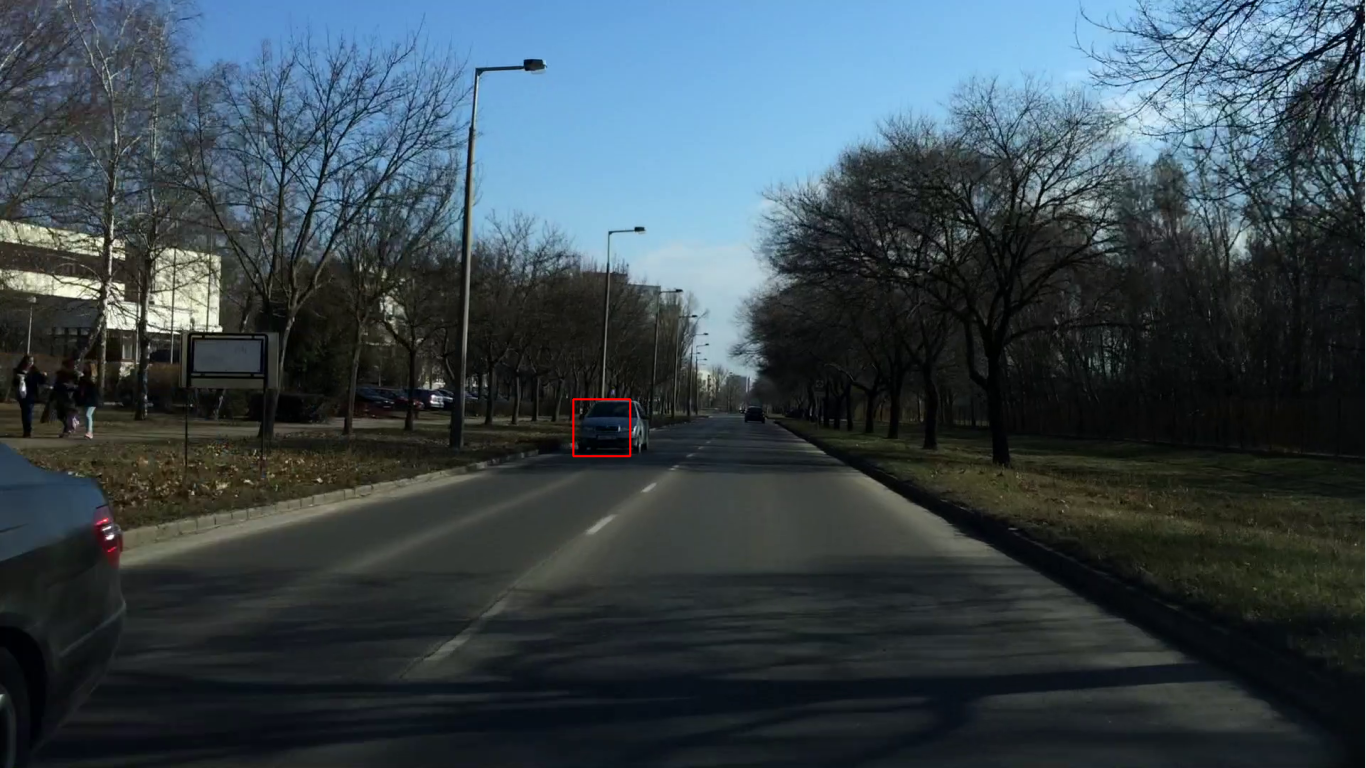
\includegraphics[width=12.6cm]{img/carredrect.png}}
\caption{The basic functionality of the object detection algorithm.}
\label{carredrect}
\end{figure}

\section{Using Data -- The Crowd-sourced Traffic Simulator}
\label{cstssect}

The aggregated output data of the RTTA was used as an input to the RCE. For this, we created a fork of the original OOCWC, and modified it. The project's name is Crowd-sourced Traffic Simulator (CSTS) and can be downloaded from GitHub \cite{csts-repo}.

The input of the RCE is a plain text file that contains lines, with each line containing a street name and the car density value on that street. Let denote the street as $s_i$ ($i=1, \dots, N$), and the corresponding intensity as $v_i$. This intensity is calculated in a point or points of the corresponding street. Later, this intensity will be the average of the measured values in that point. The RCE works on an OSM based graph where the nodes are OSM way node references. Let denote the number of OSM way node references as $n_i$ on the street $s_i$ and $s_i^j$ the $j$th OSM way node reference on the street $s_i$ ($i=1, \dots, N$, $j=1, \dots, n_i$). Then, we initialize the vehicle to the $s_i^j$ node according the following probability:

\[P(s_i^j)=\frac{v_i}{\sum_{k=1}^{N}{n_kv_k}}.\]

One can see easily that $\sum_{i=1}^{N}\sum_{j=1}^{n_i}P(s_i^j) = 1$.

So, we initialize vehicles for the first step of the simulation as measured. Then, we can observe the operation of the simulation algorithm.

To obtain this functionality, we had to extend the original OOCWC implementation with one new class. In this class, we represent the traffic that is based on real measured data. The new class is inherited from the Traffic class. The new members of this class are the measured distribution of cars and a function that initializes the vehicles (described above). As shown in Source \ref{trafobj}, we create an instance of this class if we want to initialize traffic based on measured data. In the constructor of the class, the \emph{itype} parameter must be set, identifying that we want to use measured data.

\begin{lstlisting}[language=C++,caption=Creating a RealTraffic object., label=trafobj]
traffic = new justine::robocar::RealTraffic {
      nrcars,       //Number of cars 
      shm.c_str(),  //Shared memory management
      catchdist,    //Catch distance 
      type,         //Type of traffic simulation
      itype,        //Type of car initialization  
      minutes       //Time of the simulation 
};
\end{lstlisting}

In Source \ref{nodesel}, the method of the initialization of the cars can be observed. The return value of the function is the Way Node ID of the OSM graph where we initialize the current vehicle. First, the function summarizes the ID-s (see Line \ref{nodesum}), then generates a pseudo random number (at Line \ref{noderandom}). Based on this number, we decide whether we put the car on that node or not. One example on this type of initialization can be seen in Fig.~\ref{simulinit}.

\begin{lstlisting}[language=C++,caption=Initialization., label=nodesel, escapechar={|}]
osmium::unsigned_object_id_type virtual node(){
  double no_edges = 0;
  for ( shm_map_Type::iterator iter=shm_map->begin();
        iter!=shm_map->end(); ++iter ){

      for ( auto nodeval : RealTraffic::alist[iter->first] )
        no_edges += nodeval; |\label{nodesum}|
    }
  double rand = ( double ) std::rand() / ( double ) RAND_MAX; |\label{noderandom}|
  double sum = 0.0;
  for ( shm_map_Type::iterator iter=shm_map->begin();
        iter!=shm_map->end(); ++iter ){

      for ( auto nodeval : RealTraffic::alist[iter->first] ){
          sum += ( double ) nodeval/no_edges;
          if ( sum >= rand )
            return iter->first;
        }
    }
}
\end{lstlisting}

\begin{figure}[ht!]
\centerline{
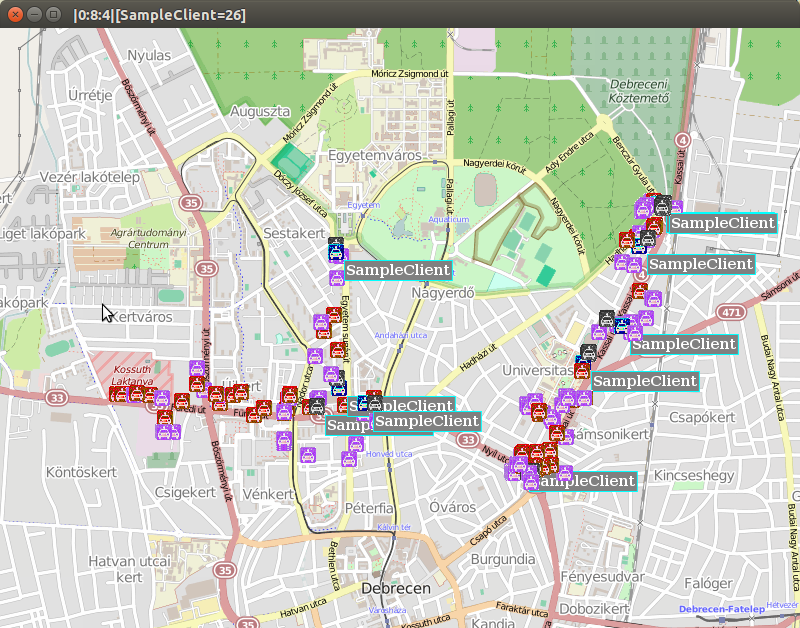
\includegraphics[width=11cm]{img/ut3.png}}
\caption{The first step of the simulation initialized based on measured data. The input file contains the following lines: Kassai \'ut 789 \textbackslash  Egyetem sug\'ar\'ut 317  \textbackslash  F\"uredi \'ut 559. Source: \cite{infocomjournal}. Base map and data from OpenStreetMap and OpenStreetMap Foundation. \copyright OpenStreetMap contributors.}
\label{simulinit}
\end{figure}

\section{Data collection conclusions}

The RTTA (according to Fig.~\ref{tetris_plan} the ASA) will be an important part of the OOCWC system. For traffic simulations, scenario analysis and effective route planning, we need real measured data, so we developed a rapid prototype application for data collection following the crowd-sensing approach. The device is based on ARM which, with the software parts, will be ready to be assembled into vehicles. We performed the initial test of the device in Debrecen and the collected data was used as an input to the RCE. The name of this device is Real-time Traffic Analyzer, the fork implementation of the OOCWC that uses collected data in the Crowd-sourced Traffic Simulator.

It is important to note that the novelty of the system is that the device is moving during measurement. We had to take this into consideration during design planning. The authors have no knowledge about such data collection device. There exist similar devices, but all are designed for fixed position. The central element of the system is the Digilent Zybo development board, which consists of an FGPA and an ARM CPU. The FPGA part handles I/O and memory, the ARM performs image processing. Because the device is moving, we had to extend the device with a GPS module. The image processing is a Haar-cascade based object classification, the videostream has a resolution of 640$\times$480. The pre-processed data, the street name and the car density value on the given street, is sent to our server application via a standard GSM module.

The measurement is a vehicle counting method that provides a density value on a given road segment or street. The application on server side collects the data, aggregates it, then assigns it to streets. The program creates a file where each line contains a street name and a density value of the given street. In the RCE, we use this density value as an initialization of the simulation. We start the simulation and observe the distribution of cars. OOCWC is a flexible system, i.e.~it is relatively easy to modify it to different applications. CSTS proves that we could modify it to operate with measured data.

We should note that the data collector system worked properly during the test phase; the object detection algorithm recognized vehicles coming from the opposite direction, could provide an accurate position and the data arrived at the server side properly. After a minor development phase, the RCE could simulate traffic that was initialized with measured data.

The Zybo board seems to have enough resources now, but if we want to extend the functionality of the system, it may run out of processing power and memory. We are planning to migrate the image processing to the FPGA part. The peripheries work fine, but we are planning to change the communication interface to LoRaWAN.\footnote{\url{https://lora-alliance.org/about-lorawan}}

LoRa is a {{\bf Lo}}ng {{\bf Ra}}nge, low power consumption radio technology that allows \textit{Internet of Things} (IoT) devices to send small data packages to large distances. We have tested the LoRaWAN network in Debrecen. The aim of this initial test was to understand how to use this communication protocol and how to assemble a LoRaWAN chip into our system. We used an RN2483-I/RM101 LoRa Transceiver Module\footnote{\url{http://ww1.microchip.com/downloads/en/DeviceDoc/50002346C.pdf}} on a corresponding RN2483 breakout panel, connected to a USB shield (see Fig.~\ref{lorahw}). During the test, we sent the current GPS coordinates of the device to the base station with a constant time interval. In Fig.~\ref{lorawan-test} two different measurements can be observed. Green waypoints indicate that the message with the corresponding GPS coordinates (the location where the message was sent) was received by the base station, red waypoints indicate lost messages. The blue waypoint indicates the base station. At the time of this test, only one base station\footnote{Thanks for the chance to use the base station to ChipCAD Kft., Hungary.} existed.  

\begin{figure}[ht!]
\centerline{
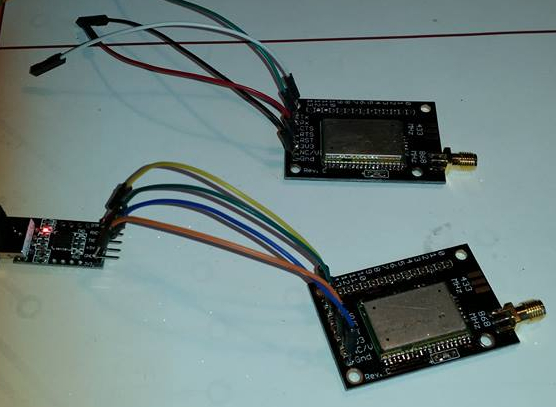
\includegraphics[width=8cm]{img/lorawan_hw.jpg}}
\caption{The LoRaWAN module applied for the test.}
\label{lorahw}
\end{figure}

\begin{figure*}[!ht]
\begin{minipage}{.54\linewidth}
\centering
\subfigure[The first initial test.\label{lorawan1}]{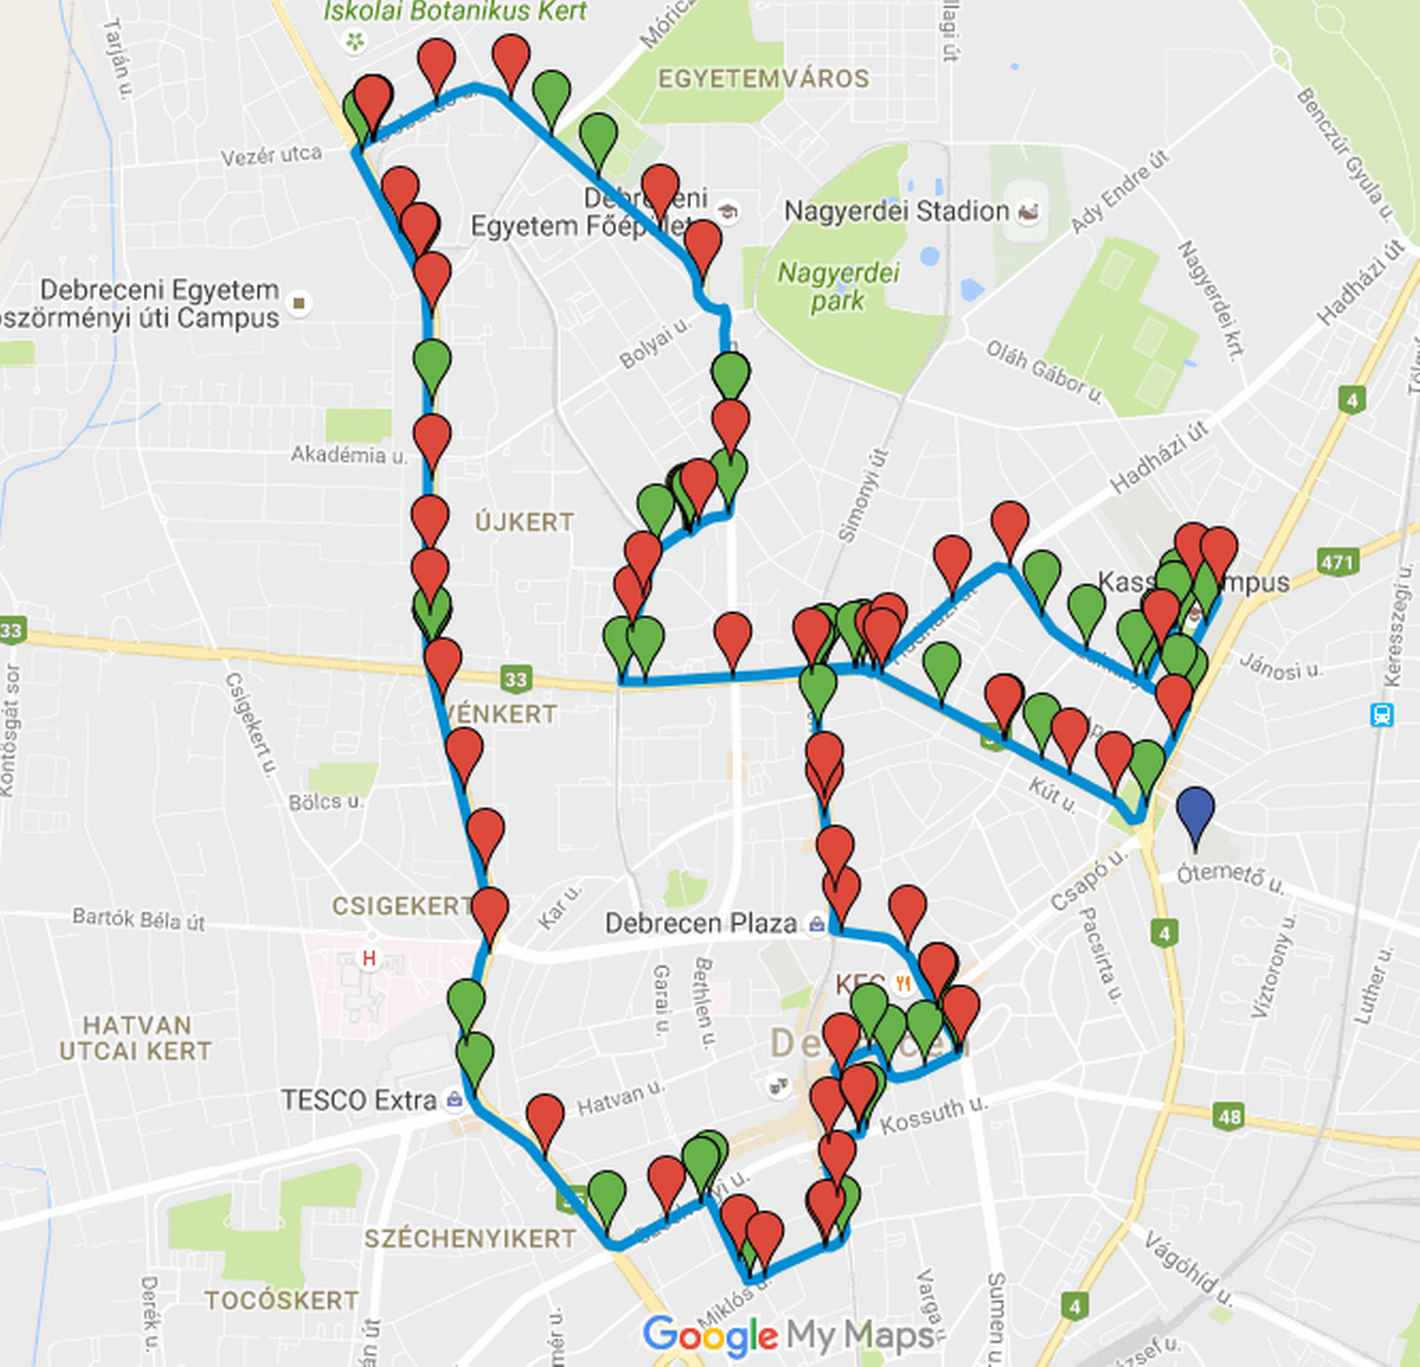
\includegraphics[width = 1\textwidth]{img/lorawan1.png}}
\end{minipage}
\begin{minipage}{.4\linewidth}
\centering
\subfigure[The second initial test.\label{lorawan2}]{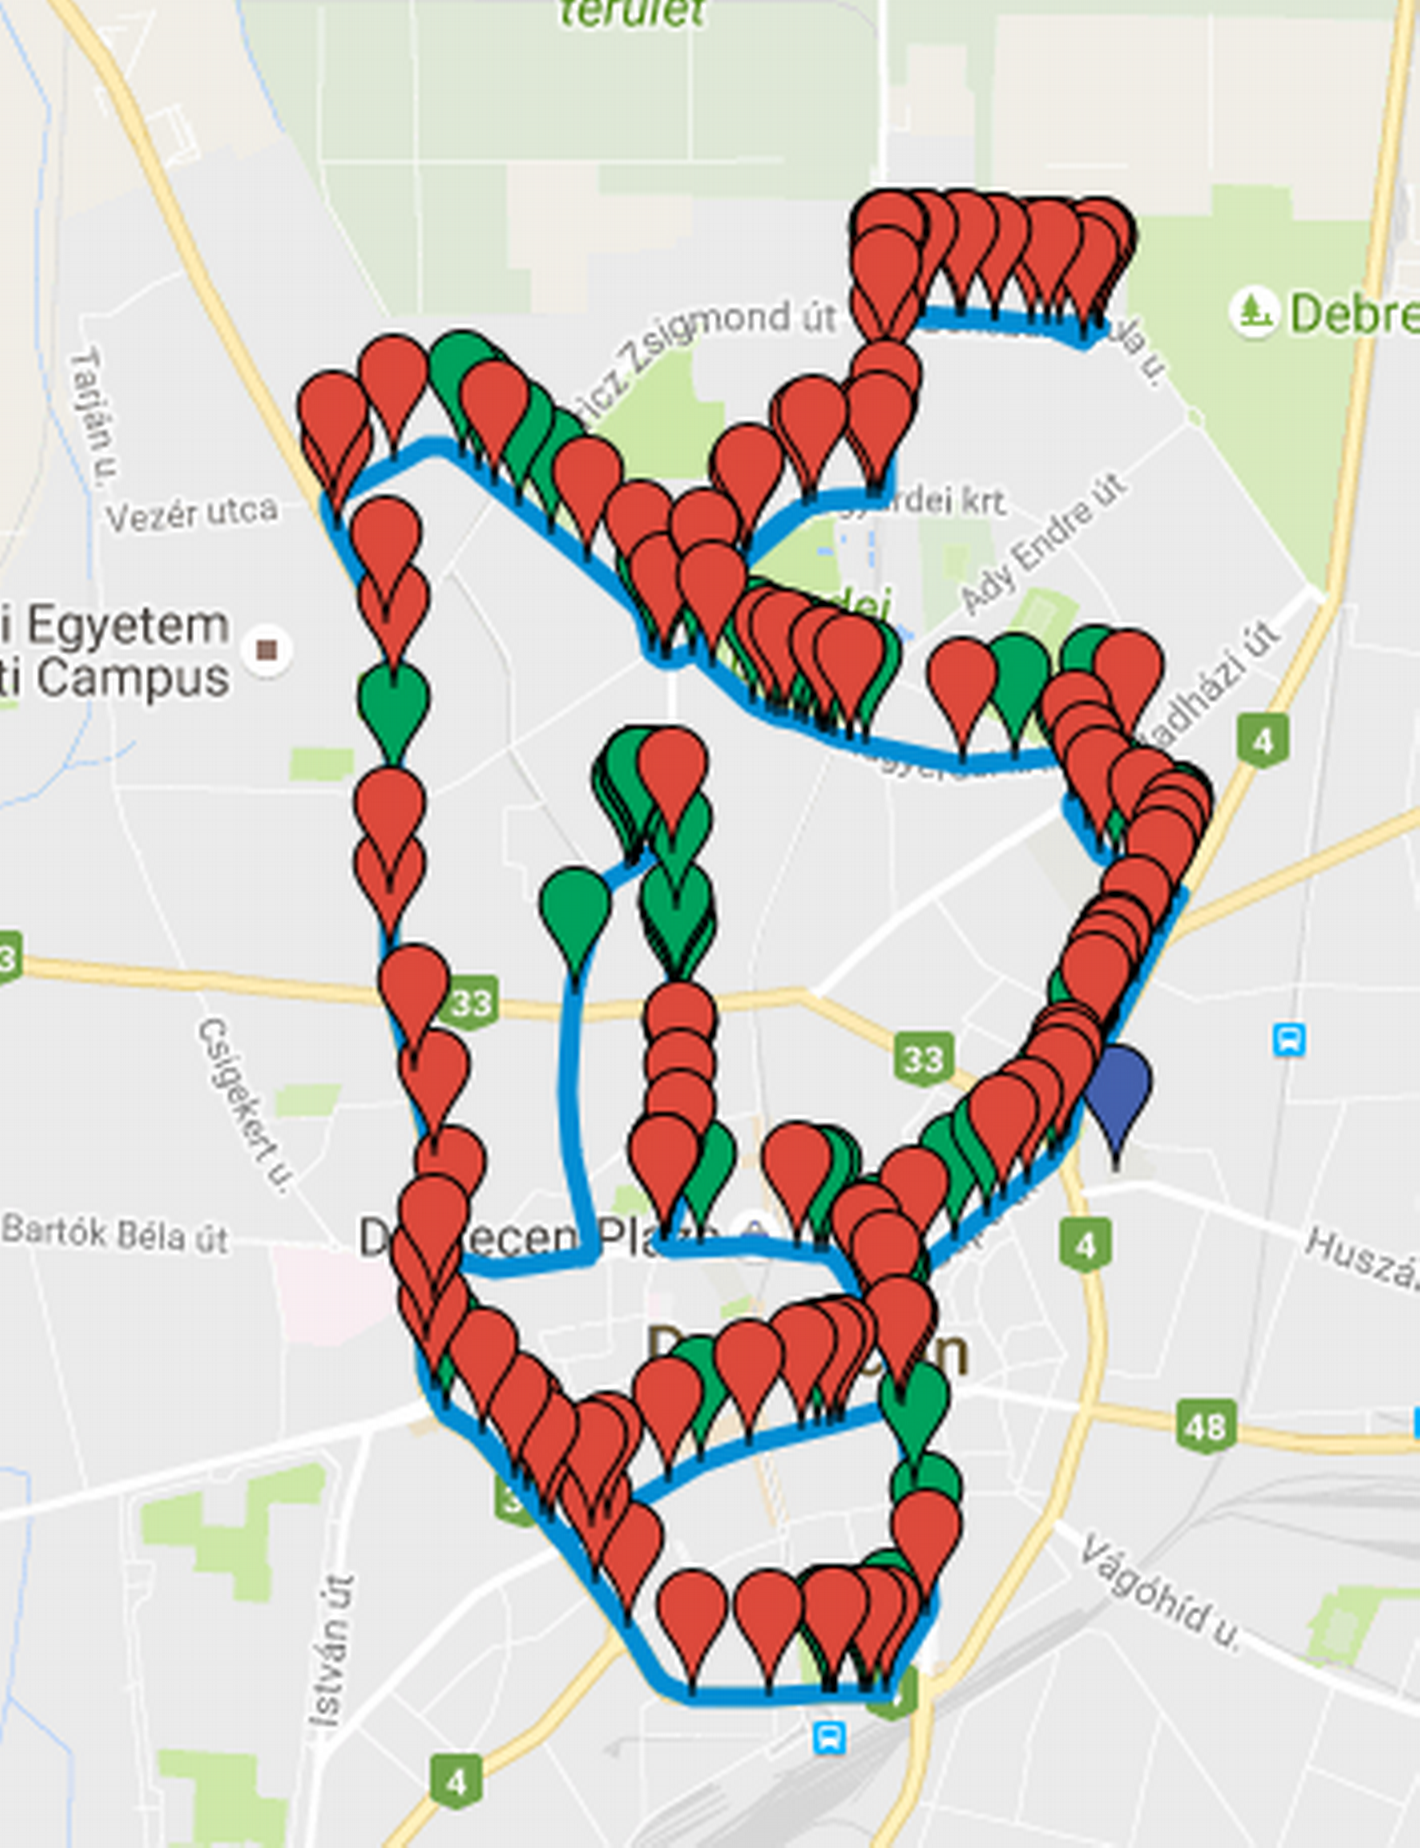
\includegraphics[width = 1\textwidth]{img/lorawan2.png}}
\end{minipage}
\centering
\caption{The results of the first initial tests of the LoRaWAN communication protocol.}\label{lorawan-test} 
\end{figure*}

\chapter{Simulation algorithms}
\label{simul}

In this section, the proposed simulation algorithm will be introduced.\footnote{Because of the length regulations of the thesis, some parts of the mathematical model are omitted for brevity. For a detailed description, see paper \cite{traffic-paper} and its longer version on arXiv \cite{besenczi2020largescale}.} The model is based on graph theory and a Markov model of probability theory. First, we show the simulation algorithm that is included in the original OOCWC system and some other simulation tools and models. Then, we describe our model in detail. We use a publicly available dataset, so we outline the concept how we use this data. After, we describe the use of OSM data in our simulation environment. Finally, we outline our results and draw some conclusions.

\section{Introduction}
In the CSTS system, the initial state of the simulation can be initialized based on measured data or some prescribed distribution (e.g.~uniform one). The former can be seen in Fig.~\ref{simulinit}; in this case, we can observe how the distribution of the cars change during the simulation. Fig.~\ref{histoder} shows the change of the distribution in the case of the simulation algorithm included in the original OOCWC version. (The simulation occurs on the map of Debrecen represented with a graph.) The $x$ axis shows the streets, the $y$ axis shows the number of cars on that street. Only streets are shown that have at least one car on it. These histograms show the number of cars on the streets of Debrecen in a descending order. It is interesting to observe that the nature of the distribution did not change during the simulation. However, another important aspect is that the order of the streets should remain the same (we require a sort of stationarity). It can be observed that the order of the streets changed during the simulation. During the test, we initialized 10,000 cars based on the measured data. This can be seen on Fig.~\ref{simultenth}.

Since the application was a prototype, some of its features were not defined or developed satisfactorily. One such feature was the traffic simulation algorithms. In this version, the simulation algorithm moves the cars quite randomly. So, when a car arrives to an intersection, it selects the next street according to uniform distribution.

\begin{figure}[!t]
    \centering
    \subfigure{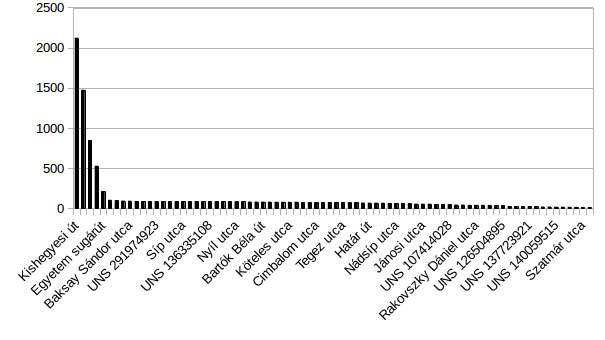
\includegraphics[width=0.65\textwidth]{img/a1.png}\label{hista}}
    \hspace{0em}
    \subfigure{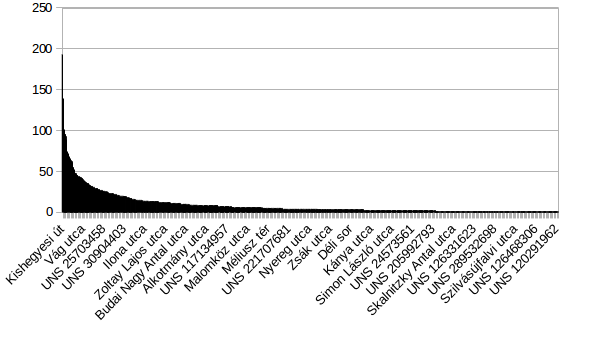
\includegraphics[width=0.65\textwidth]{img/a2.png}\label{histb}}
    \hspace{0em}
    \subfigure{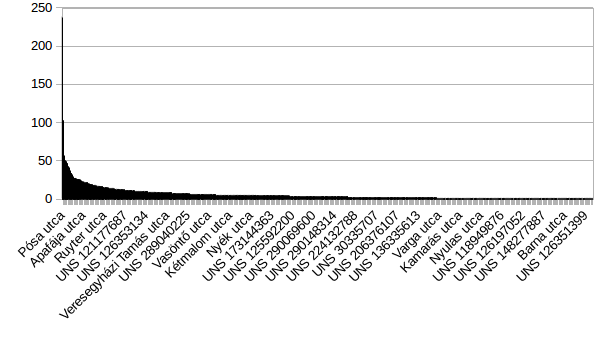
\includegraphics[width=0.65\textwidth]{img/a3.png}\label{histc}}
    \hspace{0em}
    \caption{The change of the order of the streets. The number of the street in each step is 78, 1,085 and 1,725 respectively. Source: \cite{infocomjournal}.}
    \label{histoder}
\end{figure}

\begin{figure}[ht]
\centerline{
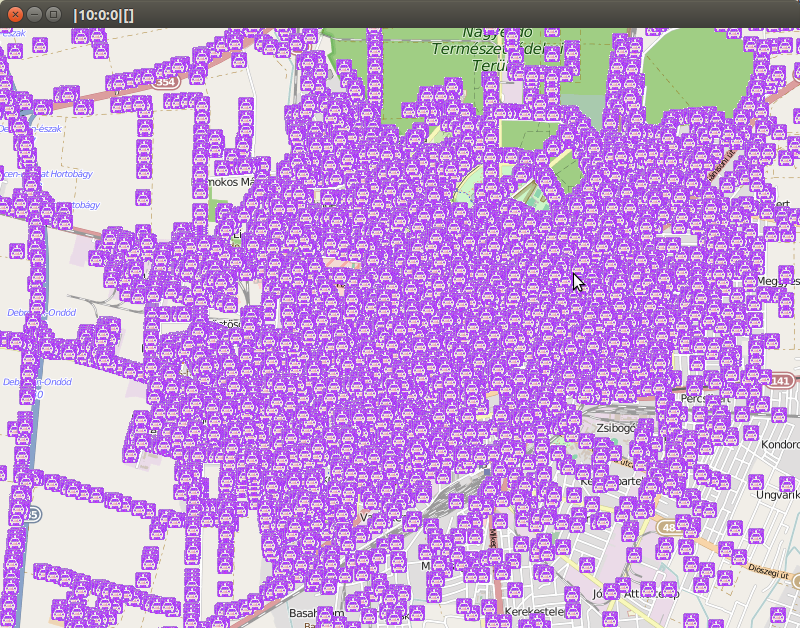
\includegraphics[width=11cm]{img/a33.png}}
\caption{Screenshot from the simulation. Source: \cite{infocomjournal}.}
\label{simultenth}
\end{figure}

In papers \cite{Crisostomietal2011}, \cite{Faizraetal2015} and \cite{Faizrahnemoon2016}, authors introduced a stochastic model that can control the traffic in an urban road network. The model is based on discrete time Markov chain on the road graph which plays the role of the state space. A transition probability matrix is introduced that describes the dynamic of the traffic while its unique stationary distribution corresponds to the traffic equilibrium (or steady) state. In this equilibrium state, the distribution of the cars on the graph remains invariant locally in time. So, this stationary distribution of the Markov chain can be interpreted as the momentary true distribution of the vehicles on the road network.

Based on the aforementioned mathematical model, we introduce the concepts of \enquote{Markov random walk}, which describes the motion of an individual vehicle, and \enquote{Markov traffic}, which describes the entire traffic on the road network, respectively. The stationary distribution of the Markov traffic will be determined as a multinomial distribution. We present how the ergodic theory of finite Markov chains implies that a dense traffic event can be approximated well by the stationary distribution of a Markov chain on the road network. We reparametrize the model by introducing the concept of two-dimensional stationary distribution which possesses equidistributed marginals that are the unique stationary distribution of the transition probability matrix, respectively. To estimate this parameter matrix the weighted least squares (WLS) estimation as a kind of composite (quasi-) likelihood methods is applied, see \cite{Hjort2008Varin}. Afterwards, we show that the WLS estimator of the two-dimensional stationary distribution can be expressed explicitly.

\section{Other simulation programs and approaches}

Several traffic simulation tools exist. Simulation of Urban Mobility \cite{SUMO2012} (or SUMO) is a portable, microscopic and continuous traffic simulation package. Aimsun\footnote{\url{https://www.aimsun.com/}} is a traffic modeling software environment that includes a mesoscopic and microscopic hybrid simulator. Multi-Agent Transport Simulation \cite{horni2016multi} or Matsim for short (version 0.8.0) is an open source software for large-scale, agent-based transport simulations. Its primary simulation algorithm is queue-based \cite{Charypara} and aims to reach an \enquote{equilibrium state} by co-evolutionary algorithms \cite{popovici2012coevolutionary}. PTV Vissim\footnote{\url{http://vision-traffic.ptvgroup.com/en-us/products/ptv-vissim/}} is a microscopic multi-modal traffic flow simulation package for traffic patterns. Although the above-mentioned applications are widely used in traffic analysis and planning, the main focus of their simulation algorithms is on microscopic traffic events. In contrast, our software system focuses only on the traffic flow of the whole city, or, to be more precise, the traffic graph.

Several approaches exist for short-term traffic flow prediction. These models are based on for example Box-Jenkins time-series analyses with ARIMA model \cite{van1996combining}, \cite{lee1999application}, \cite{stathopoulos2003multivariate}, \cite{ghosh2009multivariate}, \cite{xue2008short}, Kalman filter theory \cite{wang2005real}, \cite{ngoduy2011low}, non-parametric methods (k-NN, kernel, local regression) \cite{davis1991nonparametric}, \cite{smith2002comparison}, \cite{turochy2004relating}, \cite{smith1997traffic}, exponential smoothing \cite{messer1993advanced}, \cite{castro2009online}, spectral analysis \cite{nicholson1974prediction} or wavelets \cite{jiang2005dynamic}, \cite{xie2006wavelet}, \cite{cheng2007mining}. In addition, several approaches use machine learning and data mining techniques, such as support vector regression \cite{jeong2013supervised}, artificial neural networks \cite{chan2012neural}, \cite{park1998short}, \cite{dia2001object}, Bayesian networks \cite{sun2006bayesian} or deep learning \cite{lv2015traffic}. Some applications can be found based on computational intelligence techniques, e.g., linear genetic programming \cite{brameier2007basic} or Fuzzy logic \cite{iokibe1993traffic}, \cite{li2006type}, \cite{zhang2008short}, but seldom can we find approaches based on Markov models \cite{necula2014dynamic} and \cite{Crisostomietal2011} mentioned previously. Note that the joint application of Markov chains and large graphs to analyze the behavior of complex systems is well known in several fields, e.g., distributed systems \cite{dabrowski2011hunt}, geophysics \cite{Cavers2015Vasudevan} and biology \cite{Lesne2006}.

\section{The proposed model}
\label{model-desc}

In this section, we give a brief outline of our mathematical model.

\subsection{Basic concepts and notation}
\label{model-basics}

In this subsection, we introduce the concepts of graph theory and the theory of finite Markov chains that are necessary for our method. A textbook on graph theory is \cite{JensenGutin2007}, some textbooks on Markov chains are \cite{Asmussen2003} and \cite{Bremaud1999}.

\smallskip

\textbf{Road network, line digraph and degree distributions.} Let $G = (V,E)$ be a directed graph (digraph) where $V$ and $E$ denote the set of vertices or nodes and the set of directed edges of the graph, respectively. In the sequel, vertices are denoted by $u, v, w,$ edges are denoted by $e, f, g$. For a directed edge $e = (v,w) \in E$ we also use the notation $v \rightarrow w$. $G$ is a simple digraph, i.e.~it does not contain two or more edges that connect the same two vertices in the same direction. The digraph $G$ represents the road system of a city. More precisely, we have the following definition, see \cite{pan2013crowd}, 
\begin{definition}
A \textbf{road network} $G$ is a simple directed graph, $G = (V,E)$, where $V$ is a set of nodes representing the terminal points of road segments, and $E$ is a set of directed edges denoting road segments.

A \textbf{road segment} $e = (v,w) \in E$ is a directed edge in the road network graphs, with two terminal points $v$ and $w$. The vehicle flow on this edge is from $v$ to $w$.
\end{definition}

\begin{figure}[b!]
\centering
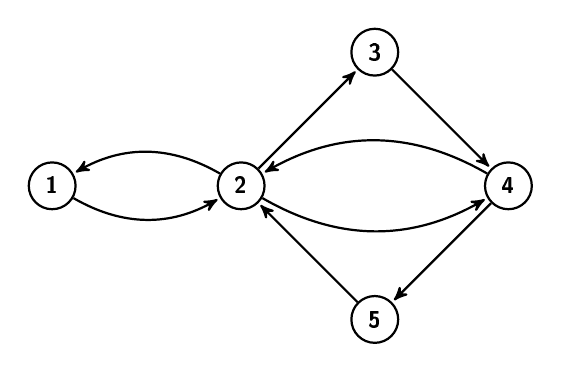
\begin{tikzpicture}[->,>=stealth',shorten >=1pt,auto,node distance=2.4cm,
                    thick,main node/.style={circle,draw,font=\sffamily\small\bfseries}]
 
  \node[main node] (3)  {3};
  \node[main node] (2) [below left of=3] {2};
  \node[main node] (1) [left of=2] {1};
  \node[main node] (4) [below right of=3] {4};
  \node[main node] (5) [below right of=2] {5};  
  \path[every node/.style={font=\sffamily\small}]
    (1) edge [bend right] node {} (2)
    (2) edge node {} (3) 
        edge [bend right] node {} (1)
        edge [bend right] node {} (4)        
    (3) edge node  {} (4)
    (4) edge [bend right] node {} (2)
         edge node {} (5)
    (5) edge node {} (2);    
\end{tikzpicture}
\caption{A simple road network.}
\label{graph-example-1}
\end{figure}
Fig.~\ref{graph-example-1} presents a simple road network.

On a road network, we allow loops but only to represent that a vehicle remains at the same node or edge after a time step. For $v \in V$ define $v^{−} := \{e \in E\, |\, \exists u \in V : e = (u, v)\}$ and $v^{+} := \{e \in E \,|\, \exists w \in V : e = (v, w)\}$. $v^{−}$ and $v^{+}$ are the sets of arrows in and out of the node $v$, respectively. Note that $deg^{−}(v) = |v^{−}|$ and $deg^{+}(v) = |v^{+}|$ is the indegree and outdegree of $v$, respectively, where $|\cdot|$ denotes the cardinality of a set. Based on this, the degree distributions on our Porto example graph can be seen in Fig.~\ref{porto-in-out}. One can see clearly that this graph is sparse in a sense that there is no node with higher indegree or outdegree than 6.

For a digraph $G$ another digraph can be associated. Let the set $V'$ of vertices of this new digraph be the set of directed edges $E$ of $G$ and let the set $E'$ of its directed edges consist of the ordered pair $(e, f)$ where $e, f \in E$ such that there exist $u, v, w \in V$ that $e = (u, v)$ and $f = (v, w)$. This associated digraph is called a directed line graph, see Section 4.5 in \cite{JensenGutin2007}, and it is denoted by $\text{L}(G) = (V', E')$. A digraph assigns the vehicles moving in a city to the vertices while a line digraph to the edges.

\smallskip

\textbf{Adjacency matrix.} We can define vectors (functions) and matrices (operators or kernels) on $V$ in the following way. Let $\balpha: V\to \mathbb{R}$ be a real function on $V$. Let $T:V\times V\to \mathbb{R}$ be a real function. Then $T$ is called matrix, operator or kernel on $V$ and induces a linear operator in the following way: for each $\balpha$, $T(\balpha)$ is defined as $T(\alpha)_u := \sum_{v\in V} t_{uv} \alpha_v$, $u\in V$. If the support of $T$ (the set $\{(u,v)\,|\, u,v\in V: t_{uv}\neq 0\}$ in $V\times V$) is a subset of $E$ ($E\cup S$) then $T$ is called $G$-subordinated in strong (weak) sense. 

Let $A = (a_{uv})_{u,v\in V} $ denote the adjacency matrix of the digraph $G$, i.e., $A$ is a matrix on $V$ and $a_{uv} = 1$ if and only if $(u,v) \in E$ and $0$ otherwise. Clearly, the support of $A$ is $E$, i.e., $A$ is a $G$-subordinated matrix in strong sense ($a_{vv} = 0$ for all $v \in V$). Note that $A$ is not necessarily symmetric. The indegree and outdegree of a vertex $v$ can be expressed by the adjacency matrix as $deg^{−}(v) = \sum_{u \in V} a_{uv}$ and $deg^{+}(v) = \sum_{u\in V} a_{vu}$. Introduce the vectors $\bd^{−} := (deg^{−}(v))_{v\in V}$ and $\bd^{+} := (deg^{+}(v))_{v \in V}$. Then, we have $\bd^{−} = A^T\textbf{1}$ and $\bd^{+} = A\textbf{1}$ where $\textbf{1} := (1)_{v \in V}$ is the constant unit function.

\smallskip

\textbf{Open road networks and their closures.} To model the possibilities that vehicles enter or leave the traffic network, $V$ is augmented by a new ideal vertex 0 which denotes the world outside of the city, see \cite{Faizrahetal2013}. Let $\overline{V} := V \cup \{0\}$. Then, additional directed edges are also added to $E$, $(v, 0)$ denotes that the vehicles can leave the city at vertex $v$, and $(0, v)$ denotes that new vehicles can enter the city at vertex $v$, where $v \in V$. The augmentation of $G$ is denoted by $\overline{G} = (\overline{V}, \overline{E})$ and it is called the closure of a road network $G$. In the rest of this section, it is assumed that the road network is closed. 

\textbf{Probability distributions and Markov kernels on road networks.} A probability distribution (p.d.)~on $V$ is the vector $\bpi := (\pi_v)_{v \in V}$ where $\pi_v \geq 0$ for all $v \in V$ and $\sum_{v \in V} \pi_v = 1$. We can think of $\pi_v$ as the proportion of the number of vehicles which drive through the crossing $v$ with respect to the whole number of vehicles in the city at a fixed time period. A Markov kernel or transition probability matrix on $V$ is defined as a real kernel $P := (p_{uv})_{u,v \in V}$ such that $p_{uv} \geq 0$ for all $u, v \in V$ and $\sum_{v \in V} p_{uv} = 1$ for all $u \in V$, i.e., $\bp_u := (p_{uv})_{v \in V}$ is a p.d.~on $V$ for all $u \in V$. The quantity $p_{uv} \in [0, 1]$ is called the transition probability from vertex $u$ to vertex $v$. Then, the sum condition for Markov kernel $P$ can be rewritten as (where the case $u = v$ is also allowed):
\begin{equation}\label{Psum}
\sum_{w:v \rightarrow w} p_{vw} + p_{vv} = 1, \quad v \in V.
\end{equation}

A p.d.~$\bpi$ on $V$ is a stationary distribution (s.d.)~of the kernel $P$ if $\sum_{u \in V} \pi_u p_{uv} = \pi_v$ for all $v \in V$. For a $G$-subordinated Markov kernel $P$ this formula, the so-called global balance equation, can be expressed as:
\begin{equation}\label{pi_eq}
\sum_{u:u \rightarrow v} \pi_u p_{uv} + \pi_v p_{vv} = \pi_v, \quad v \in V.
\end{equation}
Fig.~\ref{pi_graph} presents a Markov kernel with its s.d. From a practical point of view, subordination of a Markov kernel means that a transition probability is positive for an entry $p_{uv}$ only if an edge exists between $u$ and $v$ in the graph.

\begin{figure}[b!]
\centering
%\small
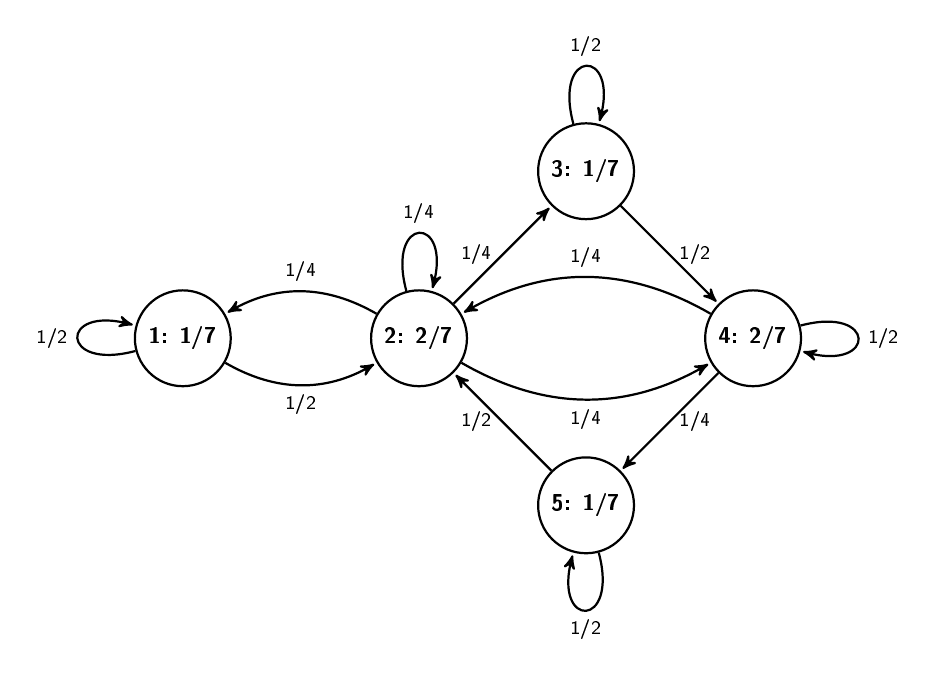
\begin{tikzpicture}[->,>=stealth',shorten >=1pt,auto,node distance=3cm,
                    thick,main node/.style={circle,draw,font=\sffamily\footnotesize\bfseries}]
 
  \node[main node] (3)  {3: 1/7};
  \node[main node] (2) [below left of=3] {2: 2/7};
  \node[main node] (1) [left of=2] {1: 1/7};
  \node[main node] (4) [below right of=3] {4: 2/7};
  \node[main node] (5) [below right of=2] {5: 1/7};  

  \path[every node/.style={font=\sffamily\scriptsize}]
    (1) edge [bend right] node [below] {1/2} (2)
          edge [loop left] node {1/2} (1)
    (2) edge node [left] {1/4} (3) 
        edge [bend right] node[above] {1/4} (1)
        edge [bend right] node[below] {1/4} (4)        
         edge [loop above] node {1/4} (2)
    (3) edge node [right] {1/2} (4)
          edge [loop above] node {1/2} (3)
    (4) edge [bend right] node [above] {1/4} (2)
         edge node [right] {1/4} (5)
          edge [loop right] node {1/2} (4)
    (5) edge node [left] {1/2} (2)
          edge [loop below] node {1/2} (5);    
\end{tikzpicture}
\caption{A Markov kernel (on edges) with its stationary distribution (on vertices) on the road network in Fig.~\ref{graph-example-1}.}
\label{pi_graph}
\end{figure}

From the viewpoint of the evaluation of our model, it will be important to choose the set $E$ for the role of the state space. Our software can only extract the number of cars on the streets, where a street is a set of edges (and it is somewhat more natural to assign vehicles to edges). For a p.d.~$(\pi^\prime_e)_{e\in E}$ on $E$ we can think of $\pi^\prime_e$ as the proportion of the number of vehicles at the road segment $e$ with respect to the whole number of vehicles in the city.

\begin{table}[t!]
\center
\caption{An example for a Markov kernel on the minimal line digraph of the road network in Fig.~\ref{graph-example-1}.}
\begin{tabular}{c|cccccccc}
&(1,2)&(2,3)&(3,4)&(4,2)&(2,1) &(2,4)&(4,5)&(5,2)\\ \hline 
(1,2)&1/2&1/4&0&0&0 &1/4&0&0\\ (2,3)&0&1/2&1/2&0&0 &0&0&0\\                 (3,4)&0&0&1/2&1/4&0 &0&1/4&0\\              (4,2)&0&1/4&0&1/2&1/4 &0&0&0\\ (2,1)&1/2&0&0&0&1/2 &0&0&0 \\                (2,4)&0&0&0&0&0&1/2&1/2&0\\                 (4,5)&0&0&0&0&0&0&1/2&1/2 \\(5,2)&0&1/4&0&0&1/8&1/8&0&1/2
\end{tabular}
\label{markov-kernel-r}
\end{table}

A Markov kernel on $E$ can be defined as a real kernel $P^\prime:=(p^\prime_{ef})_{e,f\in E}$ such that $p^\prime_{ef}\ge 0$ for all $e,f\in E$ and $\sum_{f\in E}p^\prime_{ef} = 1$ for all $e\in E$. A p.d.~$\bpi^\prime$ on $E$ is a s.d.~of the kernel $P^\prime$ if $\sum_{e\in E} \pi^\prime_e p^\prime_{ef} = \pi^\prime_f$ for all $f\in E$. Similarly to Markov kernels on $V$, we have that, for all $u\rightarrow v$,
\begin{equation}\label{Rsum}
\sum_{w:v\rightarrow w} p^\prime_{uvw} + p^\prime_{uv} =1
\end{equation}
and the global balance equation is given as:
\begin{equation}\label{rho_eq}
            \sum_{u:u\rightarrow v} \pi^\prime_{uv} p^\prime_{uvw} + \pi^\prime_{vw} p^\prime_{vw} = \pi^\prime_{vw}
\end{equation}
for all $v\rightarrow w$. (Note that $p^\prime_{uv}$ is the probability that a vehicle remains on the road segment $(u,v)$.)

An example for the Markov kernel $P^\prime$ on the minimal line digraph $\text{ML}(G)$ of the road network $G$ in Fig.~\ref{graph-example-1} is shown in Table \ref{markov-kernel-r}. Fig.~\ref{rho_graph} shows the unique stationary distribution $\bpi^\prime$ of the Markov kernel $P^\prime$. (By deleting all of the unnecessary edges, such that the remaining line digraph be still strongly connected we get the minimal strongly connected line digraph of $G$. This line digraph is denoted by $\text{ML} (G)$.)

\begin{figure}
\centering
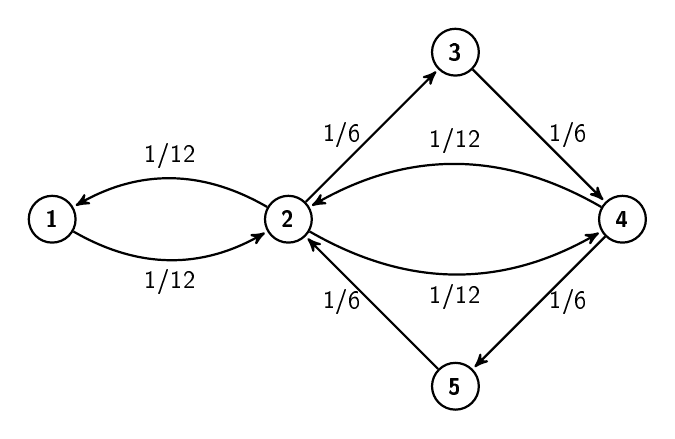
\begin{tikzpicture}[->,>=stealth',shorten >=1pt,auto,node distance=3cm,
                    thick,main node/.style={circle,draw,font=\sffamily\small\bfseries}]
 
  \node[main node] (3)  {3};
  \node[main node] (2) [below left of=3] {2};
  \node[main node] (1) [left of=2] {1};
  \node[main node] (4) [below right of=3] {4};
  \node[main node] (5) [below right of=2] {5};  

  \path[every node/.style={font=\sffamily\small}]
    (1) edge [bend right] node [below] {1/12} (2)
    (2) edge node [left] {1/6} (3) 
        edge [bend right] node[above] {1/12} (1)
        edge [bend right] node[below] {1/12} (4)        
    (3) edge node [right] {1/6} (4)
    (4) edge [bend right] node [above] {1/12} (2)
         edge node [right] {1/6} (5)
    (5) edge node [left] {1/6} (2);    
\end{tikzpicture}
\caption{The stationary distribution of the Markov kernel in Table~\ref{markov-kernel-r}.}
\label{rho_graph}
\end{figure}

We can define probability distributions and Markov kernels on open road networks as well, see section 2.2 of paper \cite{traffic-paper}.

\smallskip

\textbf{Uniqueness of stationary distribution.} The Markov kernel $P$ on $V$ is called $G$-compatible if, for any $u,v\in V$ such that $u\neq v$, $p_{uv}>0$ if and only if $(u,v)\in E$. Similarly, the Markov kernel $P^\prime$ on $E$ is called $G$-compatible if it is $\text{L}(G)$-compatible Markov kernel on $\text{L}(G)$. This is equivalent to that $p^\prime_{uvw}>0$, $u,v,w\in V$, if and only if $(u,v),(v,w)\in E$. Since $(e,f)\in E^\prime$ if and only if there exist $u,v,w\in V$ such that $e=(u,v)$ and $f=(v,w)$ we can define the $G$-compatibility of a Markov kernel $P^\prime$ as, for any $e,f\in E$ such that $e\neq f$, $p^\prime_{ef}>0$ if and only if there exist $u,v,w\in V$ such that $e=(u,v)$ and $f=(v,w)$. In other words, the compatibility of a Markov kernel means that a positive transition probability for an entry in the Markov kernel is only possible, if and only if there exists an edge between the two corresponding nodes in the graph (i.e.~there is a road segment between the two nodes in the OSM).

If $P$ is $G$-compatible, then the strong connectivity of $G$ implies that the associated graph to the Markov kernel $P$ is also strongly connected. In this case, the Markov kernel (the transition matrix) $P$ is called irreducible. Thus, by Theorem 1 in \cite{jarvis1999graph}, see also Theorem 3.1 and 3.3 in Chapter 3 of \cite{Bremaud1999} the following theorem holds.

\begin{Thm}\label{statsol}
If a road network $G$ is strongly connected, then there is a unique stationary distribution $\bpi$ ($\bpi^\prime$) to any $G$-compatible Markov kernel $P$ ($P^\prime$). Moreover, this distribution satisfies $\pi_v>0$ for all $v\in V$ ($\bpi^\prime_{uv} >0$ for all $(u,v)\in E$).
\end{Thm}

The importance of the theorem is that, all of the Markov kernels defined on a physical road network's closure that has positive transition probability on all roads, have a unique stationary distribution. Therefore, we can suppose that a real traffic which follows a Markovian dynamic has a local unique stationary distribution in a short time period. This s.d.~can be explored by observing the properties of the traffic.

\subsection{Markov random walk and Markov traffic on road networks} 
\label{Markov_traffic}

Let $(\Omega,\mathcal{A},\PP)$ be a probability space. Then a $V$-valued ($E$-valued) random variable (r.v.) is a $X:\Omega\to V$ ($Y:\Omega\to E$) measurable function, i.e., $X^{-1}(v)\in\mathcal{A}$ for all $v\in V$ ($Y^{-1}(e)\in\mathcal{A}$ for all $e\in E$). In this case, $X$ ($Y$) is a random function on the set $V$ of vertices (on the set $E$ of edges). For example, $X$ ($Y$) can be the random position of a vehicle on the road network $G$, where the position refers to the actual vertex (edge) which the vehicle belongs to. Then, $\PP(X^{-1}(v))=\PP(X=v)$ ($\PP(Y^{-1}(e))=\PP(Y=e)$) denotes the probability that a vehicle is at the vertex $v\in V$ (at the edge $e\in E$). Clearly, by $\bpi_X(v):= \PP(X=v)$, $v\in V$, a r.v.~$X$ induces a p.d.~$\bpi_X$ on $V$. Similarly, by $\bpi^\prime_Y(e):= \PP(Y=e)$, $e\in E$, a r.v.~$Y$ induces a p.d.~$\bpi^\prime_Y$ on $E$. 

A sequence $\{X_t\}_{t\in\mathbb{Z}_+}$ of $V$-valued r.v.'s is a Markov chain on the state space $V$ if the Markov property holds:
\begin{equation*}
\begin{aligned}
         \PP(X_t=v_t | X_{t-1}=v_{t-1},\ldots, X_0=v_0) \\ =  \PP(X_t=v_t | X_{t-1}=v_{t-1})
\end{aligned}
\end{equation*} 
for all $t\in\mathbb{N}$, $v_0,\ldots,v_t\in V$. If $X,X^\prime$ are $V$-valued r.v.'s then for the conditional distribution $P=(p_{v v^\prime})_{v,v^\prime\in V}$, $p_{v v^\prime}:=\PP(X=v | X^\prime=v^\prime)$, $v,v^\prime\in V$, we shall also use the notation $X|X^\prime$. Clearly, $X|X^\prime$ is a Markov kernel on $V$. Similarly, a Markov chain $\{Y_t\}_{t\in\mathbb{Z}_+}$ of $E$-valued r.v.'s can also be defined through the Markov kernel $Y|Y^\prime$ on the state space $E$.

The Markov random walk and the Markov traffic defined in the following way.

\begin{definition}
Let the road network $G$ be strongly connected and let $P$ be a $G$-compatible Markov kernel on $V$ with unique s.d.~$\bpi$. Moreover, let $\{X_t\}_{t\in\mathbb{Z}_+}$ be a Markov chain on $V$ such that $\bpi_{X_0}=\bpi$ and $X_t|X_{t-1} \sim P$ for all $t\in\mathbb{N}$. 

Then, $\{X_t\}_{t\in\mathbb{Z}_+}$ is called \textbf{Markov random walk} on the road network $G$ with Markov kernel $P$.

The set of $k$ ($k\in\mathbb{N}$) mutually independent Markov random walks on $G$ with Markov kernel $P$ is called \textbf{Markov traffic} of size $k$ and it is denoted by the quadruple $(G,P,\bpi,k)$.
\end{definition}

Similarly, $\{Y_t\}_{t\in\mathbb{Z}_+}$ is a Markov random walk on the line road network if it is a Markov chain on the state space $E$ such that $\bpi^\prime_{Y_0}= \bpi^\prime$ and $Y_t|Y_{t-1}\sim P^\prime$  for all $t\in\mathbb{N}$.

A Markov random walk is an individual Markov traffic with $k=1$ in the sense that it describes the movement of a random vehicle which follows the stochastic rules defined by the Markov kernel. 

We also have results regarding the ergodicity of Markov traffic, see paper \cite{traffic-paper}.

\smallskip

\textbf{Two-dimensional stationary distribution.} Introduce the two-dimensional distribution $Q=(q_{uv})$ on $V\times V$ as $q_{uv}:=\pi_u p_{uv}$, $u,v\in V$. Then, $Q$ is a two-dimensional stationary distribution on $G$ in the following sense: 

\begin{definition}\label{two_stat}
A matrix $Q=(q_{uv})_{u,v\in V}$ is called \textbf{two-dimensional stationary distribution} on $G$ if (i) $q_{uv}\ge 0$ for all $u,v\in V$ and $q_{uv}=0$ for all $u,v\in V$ such that $(u, v)\notin E\cup S$ (i.e., $Q$ is weakly $G$-subordinated); (ii) $\sum_{u,v\in V}q_{uv} = 1$ (i.e., $Q$ is a normalized matrix on $V$); and (iii) $\sum_{v\in V} q_{uv} = \sum_{v\in V} q_{vu}$ for all $u\in V$ (i.e., $Q$ has equidistributed marginals). \end{definition}

\begin{figure}[t!]
\centering
%\small
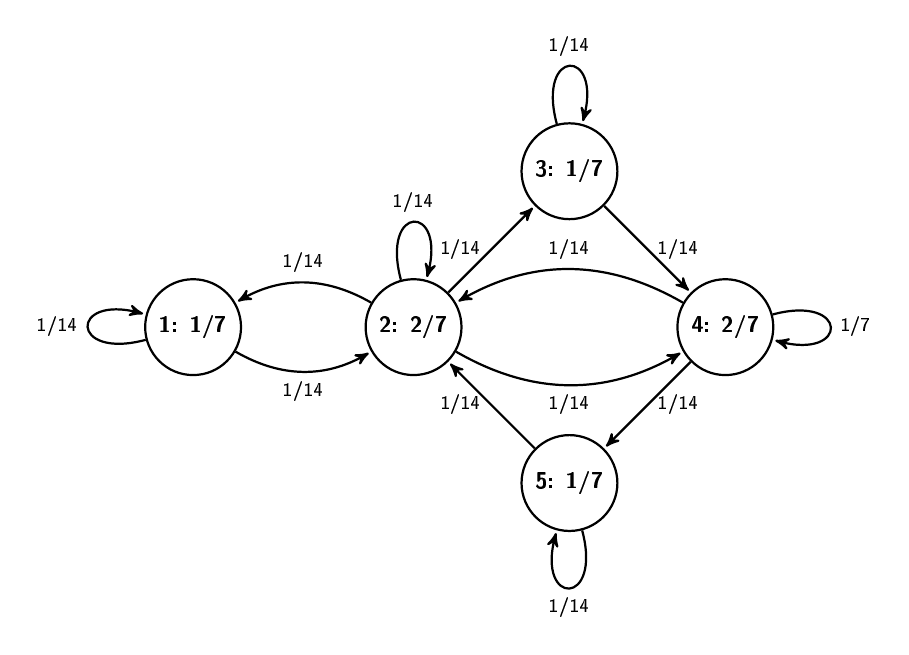
\begin{tikzpicture}[->,>=stealth',shorten >=1pt,auto,node distance=2.8cm,
                    thick,main node/.style={circle,draw,font=\sffamily\footnotesize\bfseries}]
 
  \node[main node] (3)  {3: 1/7};
  \node[main node] (2) [below left of=3] {2: 2/7};
  \node[main node] (1) [left of=2] {1: 1/7};
  \node[main node] (4) [below right of=3] {4: 2/7};
  \node[main node] (5) [below right of=2] {5: 1/7};  

  \path[every node/.style={font=\sffamily\scriptsize}]
    (1) edge [bend right] node [below] {1/14} (2)
          edge [loop left] node {1/14} (1)
    (2) edge node [left] {1/14} (3) 
        edge [bend right] node[above] {1/14} (1)
        edge [bend right] node[below] {1/14} (4)        
         edge [loop above] node {1/14} (2)
    (3) edge node [right] {1/14} (4)
          edge [loop above] node {1/14} (3)
    (4) edge [bend right] node [above] {1/14} (2)
         edge node [right] {1/14} (5)
          edge [loop right] node {1/7} (4)
    (5) edge node [left] {1/14} (2)
        edge [loop below] node {1/14} (5);  
\end{tikzpicture}
\caption{The two-dimensional stationary distribution (on edges) with its equidistributed marginals (on vertices) on the road network in Fig.~\ref{graph-example-1} for the Markov kernel in Fig.~\ref{pi_graph}.}
\label{2D_dist_toy}
\end{figure}

Property (iii) states that the two (row-wise and column-wise) marginal distributions of a two-dimensional stationary distribution on $G$ coincide with each other. The distribution $Q$ can be visualized on the edges, see, Fig.~\ref{2D_dist_toy} for the toy example and Fig.~\ref{porto_stat_dist} in case of the Porto example discussed later. 

Denote by $\mathcal{cQ}$ the set of two-dimensional stationary distributions on $G$. For a positive $Q\in\mathcal{cQ}$, let us define
\begin{equation}\label{QtoP}
\begin{aligned}
        \pi_u := &\sum_{v\in V} q_{uv} = \sum_{v\in V} q_{vu}, \quad u\in V, \qquad
        \\ p_{uv} := &\frac{q_{uv}}{\pi_u} ,\quad u,v\in V.
\end{aligned}
\end{equation} 

Then, $P=(p_{uv})$ defines a $G$-compatible Markov kernel with stationary distribution $\bpi$ on $G$. Thus, a Markov traffic defined by the quadruple $(G,P,\bpi,k)$ can be introduced by an equivalent way through the triplet $(G,Q,k)$.

\subsection{Statistical inference for Markov traffic using mobile sensors}
\label{inference}

The statistical analysis of a traffic system in our case means the estimation of the quadruple $(G,P,\bpi,k)$ or the triplet $(G,Q,k)$ using observed data. The exploration of the road network $G$ has already been done by a few organizations, in our example, we use OpenStreetMap data. In this section, we show a method for estimating the two-dimensional stationary distribution $Q$ using mobile sensor data. (By (\ref{QtoP}), the estimators for $P$ and $\bpi$ can be easily derived from an estimator of $Q$.) In this case, we have trajectories data which consists of the sequences of consecutive geographical points, like in the Taxi Trajectory Prediction dataset, see section \ref{public-dataset}. It is important to note that it is not a simple task to fit GPS-based trajectory data to the vertices of a road network $G$, see section \ref{OSM-graph}. We suppose that the size $k$ of the traffic is known.

Suppose that, for a Markov traffic, we observed a random sample of trajectories  $\{X^i\}$, $i=1,\ldots,k$, of size $k$ defined by $X_1^i\Rightarrow X_2^i\Rightarrow\ldots\Rightarrow X_{n_i}^i$, $i=1,\ldots,k$, where $n_i$ denotes the length of the $i$-th trajectory. (For a pair $u,v\in V$ the notation $u\Rightarrow v$ will mean that $(u,v)\in E\cup S$, i.e., either $u\rightarrow v$ or $u=v$.) Let $n:=n_1+\ldots +n_k$ be the total sample size. Define the total two-dimensional consecutive empirical frequencies as:
\begin{equation}\label{2freq}
    n_{uv}:= \sum_{i=1}^k n_{uv}^i,
\end{equation}     
$u,v\in V$, where the trajectory-wise two-dimensional consecutive empirical frequencies, $i=1,\ldots,k$, are defined as
\[
    n_{uv}^i := \sum_{j=1}^{n_i-1} I(X_j^i=u,X_{j+1}^i=v),
\] 
$u,v\in V$. Plainly, $n_{uv}^i$ denotes the number of consecutive $(u,v)$ ($u,v\in V$) pairs in the $i$-th trajectory. Clearly, $N= \sum_{i=1}^k N_i$ and we have
\begin{equation}\label{corr_sample_size}
    \sum_{u,v:u\Rightarrow v} n_{uv} = n-k,
\end{equation}
where $n-k$ is the corrected sample size. Introduce
\[
    s_v := \sum_{i=1}^k I(X_1^i=v), \quad
          e_v := \sum_{i=1}^k I(X_{n_i}^i = v),
\] 
$v\in V$, i.e., $s_v$ denotes the number of trajectories which start at vertex $v$ and $e_v$ denotes the number of trajectories which terminate at vertex $v$, respectively. Denote the one-dimensional marginal frequencies of $N$ by $n_{v+}:=\sum_{u\in V} n_{vu}$ and $n_{+v}:=\sum_{u\in V} n_{uv}$, $v\in V$. We obtain that
\begin{equation}\label{start_end}
    n_{v+}+e_v = n_{+v} + s_v = n_v :=\sum_{i=1}^k \sum_{j=1}^{n_i} I(X_j^i=v)
\end{equation} 
for all $v\in V$, where $n_v$ denotes the number of vertices $v$ in all trajectories. Finally,
\begin{equation}\label{start_end_sum}        
    \sum_{v\in V}  s_v = \sum_{v\in V}  e_v = k.
\end{equation} 
Define the vectors $\bs$ and $\be$ on $V$ as $\bs:=(s_v)_{v\in V}$ and $\be:=(e_v)_{v\in V}$, respectively. Then, \eqref{start_end_sum} implies that $\textbf{1}^\top (\be -\bs) = 0$, i.e., the vectors $\be -\bs$ and $\textbf{1}$ are orthogonal.

Let $A=(a_{uv})_{u,v\in V}$ and $B=(b_{uv})_{u,v\in V}$ such that $a_{uv}=b_{uv}=0$ for all $u,v\in V$ where $u\nRightarrow v$, i.e., let $A$ and $B$ be weakly $G$-subordinated matrices. The distance between $A$ and $B$ is defined as 
\[
    \| A-B\|_G := \left(\sum_{u,v:u\Rightarrow v} |a_{uv} - b_{uv}|^2\right)^{1/2}.
\]
In fact,  $\| \cdot\|_G$ is the Frobenius norm of the matrices of dimension $|V|\times |V|$ which vanish on the entries outside of $E\cup S$.

Based on $k$ number of trajectories, using the Frobenius norm, the optimality criterion is defined as the weighted sum of squared errors (SSE):
\begin{equation}\label{square_error}
    \text{SSE}(M,\bw\,|\,\bN) :=  \sum_{i=1}^k w_i^{-1} 
    \|N_i- w_i M\|_G^2,
\end{equation}
where $M$ is a non-negative parameter matrix satisfying assumptions (i) and (iii) of Definition \ref{two_stat}, $\bw=(w_i)_{i=1,\ldots,k}$ are non-negative unknown weights, i.e., $\sum_{i=1}^k w_i=1$, and $\bN:=(N_i)_{i=1,\ldots,k}$ denotes the data, where $N_i$ is the two-dimensional consecutive empirical frequency matrix for the $i$th trajectory, see \eqref{2freq}. The statistical inference for a Markov traffic means the minimization of the objective function SSE in its parameters $M$ and $\bw$ deriving the weighted least squares (WLS) estimators $\widehat{M}_{\textrm{WLS}}$ and $\widehat{\bw}_{\textrm{WLS}}$. Then, the WLS estimator of $Q$ is defined as $\widehat{Q}_{\textrm{WLS}}:= n_{\textrm{eff}}^{-1}\widehat{M}_{\textrm{WLS}}$ where $n_{\textrm{eff}} := (\textbf{1}^\top \widehat{M}_{\textrm{WLS}}\textbf{1})$ is the so-called effective sample size.

The main theorem of this section is the following.

\begin{Thm}\label{main_thm}
There is a unique pair $(\widehat{M}_{\textrm{WLS}},\widehat{\bw}_{\textrm{WLS}})$ which minimizes the weighted sum of squared errors SSE defined in \eqref{square_error}. These WLS estimators are derived as
\[
    \widehat{w}^i_{\textrm{WLS}} :=  
    \frac{\Vert N_i\Vert_G}{\sum_{j=1}^k \Vert N_j\Vert_G},
\]
$i=1,\ldots,k$, and
\[
    \widehat{M}_{\textrm{WLS}}:= N+(\textbf{1}\blambda^\top -\blambda\textbf{1}^\top)\circ A,
\] 
where $\blambda = (\lambda_v)_{v \in V}$ is called Lagrange vector and defined as a unique solution to the linear equation $L\blambda = \bs-\be$ and $\circ$ denotes the entrywise (Hadamard) product of matrices, $L$ is the symmetric unnormalized graph Laplacian matrix of $G$, and defined as $L:= D - A-A^\top$, see \cite{von2007tutorial}, where $A$ denotes the adjacency matrix of $G$ and $D:=\diag\{\bd^{+} + \bd^{-}\} $.
\end{Thm}

The estimation theory of finite Markov chains has a wide literature, see \cite{billingsley1961}. In the traditional ML approach, the estimators have a few problems and they can be applied with limited success for our purposes. Firstly, they are based on only one long trajectory (or realization). In a real traffic dataset this is quite rare. Usually, there is a large number of relatively short trajectories, like in the Taxi Trajectory Dataset, where the number of trajectories is above 80,000, the mean length is 40 and the maximum length is 2,000, see Table~\ref{desc-stat-table}. During the evaluation of our model, we will mimic this on small and medium size road networks, see section \ref{evaluation}. Secondly, the global balance equation holds only asymptotically, i.e., when the sample size tends to infinity. The inaccuracy in the global balance equation is not too large, but, this small bias can cause significant difference from the \enquote{true} stationary distribution in the simulation. Thirdly, the trajectories are biased during a short time period. In the morning, the vehicles are moving from the residential districts to the business districts of the city and they are moving back in the afternoon. In other words, the traffic has a definite direction on the road network. Fig.~\ref{tr_points_end} shows this behavior clearly by the distribution of the elements of the traffic direction vector $\bs-\be$ while Fig.~\ref{tr_points_start} shows their spatial distribution. We can handle these problems with our proposed WLS estimator. $\widehat{Q}_{\textrm{WLS}}$ is taking account of more than one trajectory with their length. In addition, it can correct the bias caused by the unbalanced sampling of trajectories on the road network.

Our proposed $\widehat{Q}_{\textrm{WLS}}$ (or $\widehat{M}_{\textrm{WLS}}$) estimator consists of two parts. First, the na\^ ive estimator for the distribution of the consecutive pairs in trajectories based on the empirical frequencies, and second, a correction term ensuring that $\widehat{Q}_{\textrm{WLS}}$ (or $\widehat{M}_{\textrm{WLS}}$) has equidistributed marginals. This second part depends on the Laplacian matrix of the road graph and the traffic direction vector. It is important to note that all statistics (two-dimensional consecutive frequencies, starting and ending frequencies) can be computed by counting, which is a very effective way and can be applied for big data, as well.

All mathematical methods presented in this section can be downloaded and tested. See Appendix, \cite[/model-sources/Markovkernel]{csts-repo} and the rest of this chapter.

\section{Public datasets}
\label{public-dataset}

In our terminology, a trajectory (or trace) is a sequence of geographical data (coordinates with timestamp) of the path of a vehicle, moving from a start to an end point. For our experiments, we needed a dataset of trajectories that conforms with the following criteria:

\begin{itemize}
\item Contains complete trajectories, so trajectories that contains only the start and the end point are not suitable.
\item Trajectories must be sampled in a high frequency, the distance between adjacent measured points should not be too large (10 meters is acceptable, but 100 meters is not).
\item The dataset should cover a long enough time period and the number of trajectories per day should be in the order of thousands.
\item Since the OOCWC operates on cities, the dataset should cover an urban area well.
\item Vehicles should not follow a fixed route, e.g., bus lanes are not suitable.
\item Publicly available and can be used for research purposes.
\end{itemize}

We observed several candidates, many datasets contained only the start and end points, e.g., New York City Taxi Trip Data,\footnote{\url{http://www.datadrivenstanford.org/features/nyc-taxi-data/}} TLC Trip Record Data,\footnote{\url{https://www1.nyc.gov/site/tlc/about/tlc-trip-record-data.page}} Uber TLC FOIL Response\footnote{\url{https://github.com/fivethirtyeight/uber-tlc-foil-response}}. Another example that is not suitable is the T-Drive trajectory dataset, because it was created using an average sampling interval of 177 seconds, so the average distance between two points is 623 meters.

We found two suitable datasets, one is the Uber GPS Traces, the other is the Taxi Trajectory Prediction from Kaggle\footnote{\url{https://www.kaggle.com/c/pkdd-15-predict-taxi} \url{-service-trajectory-i}}. The Uber dataset covers one week and contains 25,000 trajectories from San Francisco, CA, USA. Its sampling rate is 4 seconds. The Taxi Trajectory Prediction dataset covers one year and is split into training and test sets. The training set contains 1,710,670, the test set contains 320 trajectories collected in Porto, Portugal. The sampling rate was 15 seconds. Because of its much larger size, we use the Taxi Trajectory Prediction dataset.

As a first step of processing the data, we filtered the dataset between the coordinates W8.6518, W8.5771, N41.1129, N41.1756 (see Fig.~\ref{porto-map}), and trajectories that have a time of start between 8-9 am. The size of the area is 6.274 km $\times$ 6.963 km = 43.68 km$^2$, the set contains 82,345 trajectories. Features that are not relevant for us, such as origin of call, costumer IDs, etc, are omitted. Most samples are around the length of 41 coordinates, the longest contains 2,324 points. Some descriptive statistics of the dataset are shown in Fig.~\ref{desc-stat_dataset-1} and Table \ref{desc-stat-table}, see \cite{dssv-talk}.

\begin{figure*}[h!]
\begin{minipage}{.495\linewidth}
\centering
\subfigure[Histogram of number of sample points per trajectories. The grey
bar on the right represents trajectories with more than 200 sample points.
On the average, a trajectory consists of 40 sample points and takes
${\approx}10$ minutes.\label{pkdd15_sample_points}]{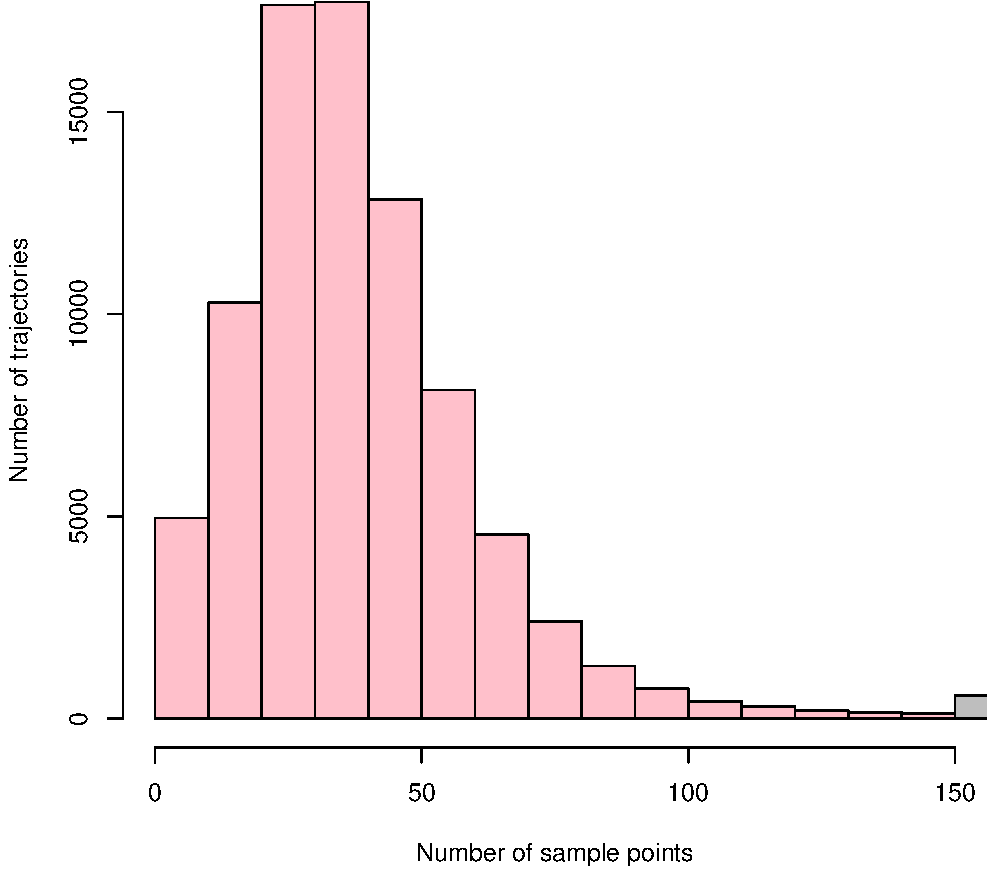
\includegraphics[width = .9\textwidth]{img/pkdd15_sample_points.pdf}}
\end{minipage}
\begin{minipage}{.495\linewidth}
\centering
\subfigure[Histogram of trajectory lengths. The grey bar on the right represents
trajectories longer than 12,500 meters. The average trajectory length is
3,628.93 meters.\label{pkdd15_trajectory_length}]{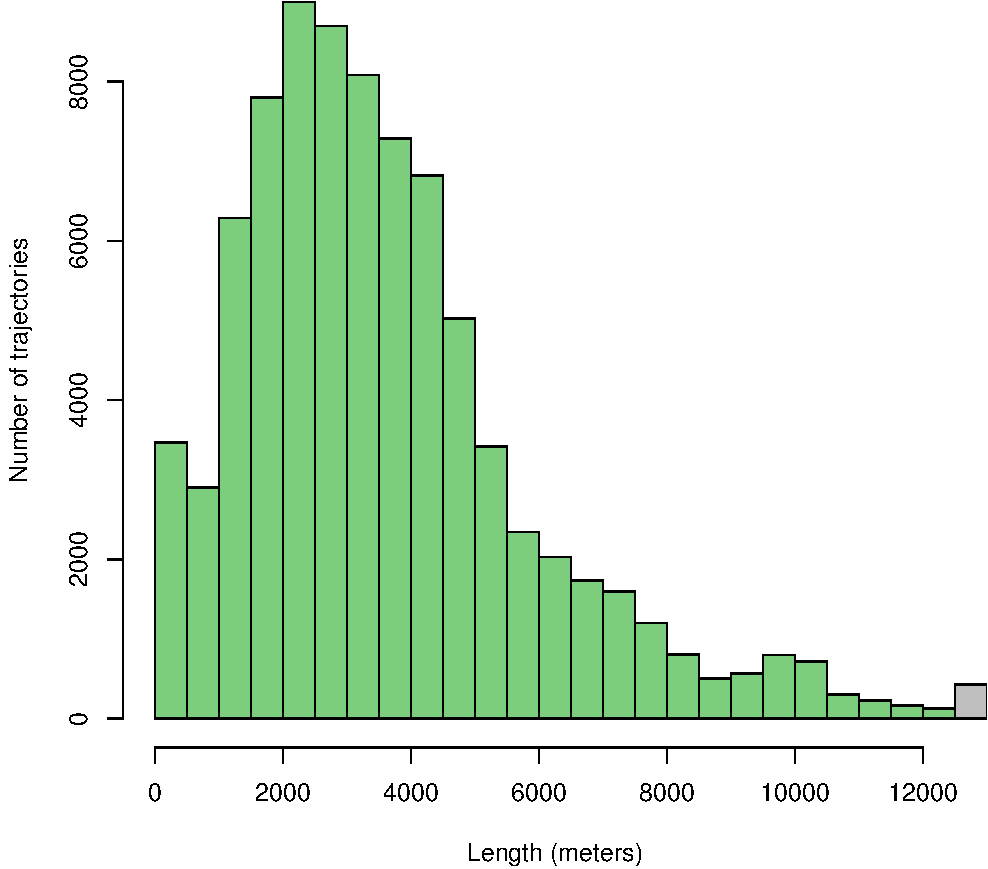
\includegraphics[width = .9\textwidth]{img/pkdd15_trajectory_length.pdf}}
\end{minipage}
\centering
\caption{Some statistics of the dataset. Source: \cite{traffic-paper}.}\label{desc-stat_dataset-1} 
\end{figure*}

\begin{table}[t!]
\centering
\caption{Descriptive statistics of lengths of trajectories. (82,345 total.)}
\label{trajectory-lenght-stat} 
\begin{tabular}{l|c c}
Name of statistics  & Distance in points & Distance in meters \\ \hline
Mean                & 39.53     & 3,628.93    \\ 
Median              & 35     & 3,176.786   \\ 
Mode                & 34     & 0         \\ 
Standard Deviation  & 31.64  & 2,408.93  \\ 
Kurtosis            & 473.28 & 9.9  \\ 
Skewness            & 12.11   & 1.78  \\ 
Minimum             & 2      & 0         \\ 
Maximum             & 2,324   & 61,055.58  \\ 
\end{tabular}
\label{desc-stat-table}
\end{table}

\begin{figure}[t!]
\centering
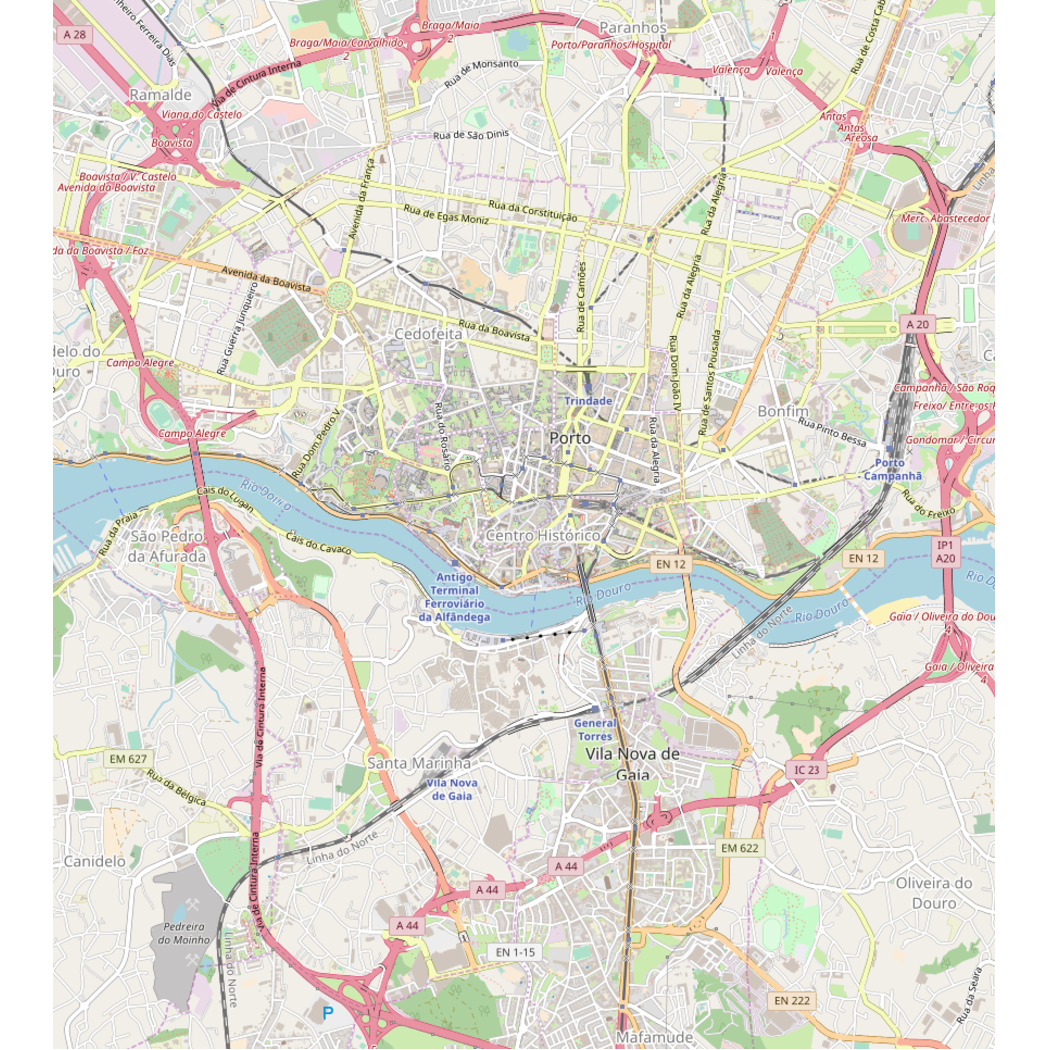
\includegraphics[width = .7\textwidth]{img/pkdd15_map_subset.pdf}
\caption{Map of the area covered by the selected subset of the dataset. The size of the area is 6.274 km $\times$ 6.963 km = 43.68 km$^2$. \copyright OpenStreetMap contributors.}
\label{porto-map}
\end{figure}
\section{Graphs from OSM}
\label{OSM-graph}

The first step of processing is to create a graph of Porto from the same bounding box that we used for subsetting the data. Since we only need nodes that can be reached by vehicles, we select only specific nodes of the OSM. For every node we store its coordinates and its OSM ID. Nodes will be vertices in the graph. The weight of the edges is the square distance between the two nodes. We used the pyosmium library\footnote{\url{https://osmcode.org/pyosmium/}} for processing OSM files and the NetworkX library\footnote{\url{https://networkx.github.io/}} for creating the graph. The resulting graph has 33,961 nodes and 53,126 edges. The indegree and outdegree distribution (see section \ref{model-basics}) of the Porto traffic graph can be observed in Fig.~\ref{porto-in-out}. Various distributions of the trajectory points (all, difference of start points and end points, histogram of difference) is shown in Fig.~\ref{ttp-points}.

When the graph is ready, we process the list of trajectories. First, we convert the GPS coordinates of the points to OSM node IDs. We simply search for the closest OSM node. Hence, the resulting node will be in the same domain as the graph built earlier. The coordinates are sampled in regular time interval, so the trajectories are not aligned to OSM data (and with the graph built previously). So, we need to interpolate the data to fit our graph. For this, we run Dijkstra's shortest path on our graph between every node ID. In some cases, because of OSM errors, there is no route between two nodes that are extracted from the dataset. In this case, we split that trajectory into two chunks. 

\begin{figure}[!t]
    \centering
    \subfigure[Indegree distribution (vertices).]{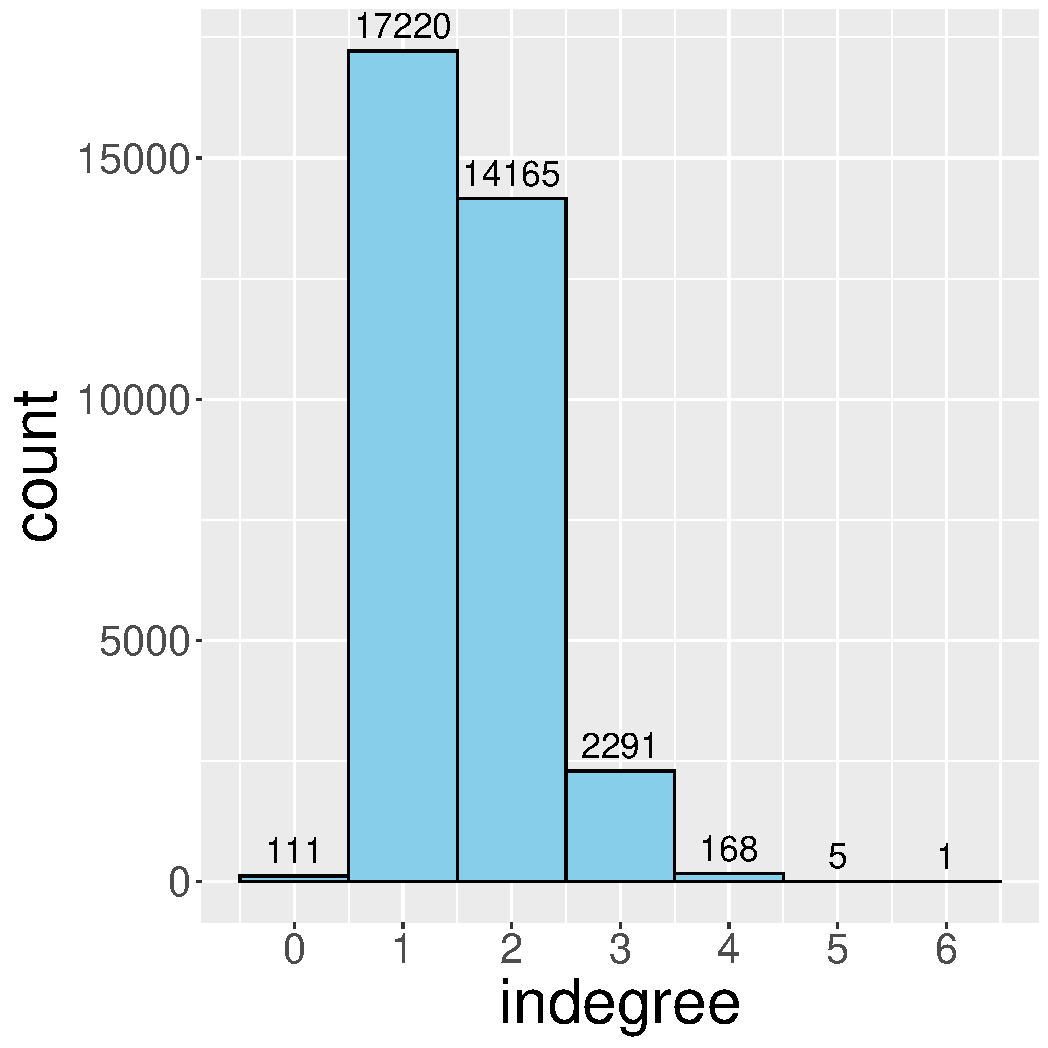
\includegraphics[width=0.4\textwidth]{img/indegree.pdf}\label{ind_v}}
    \hspace{0em}
    \subfigure[Outdegree distribution (vertices).]{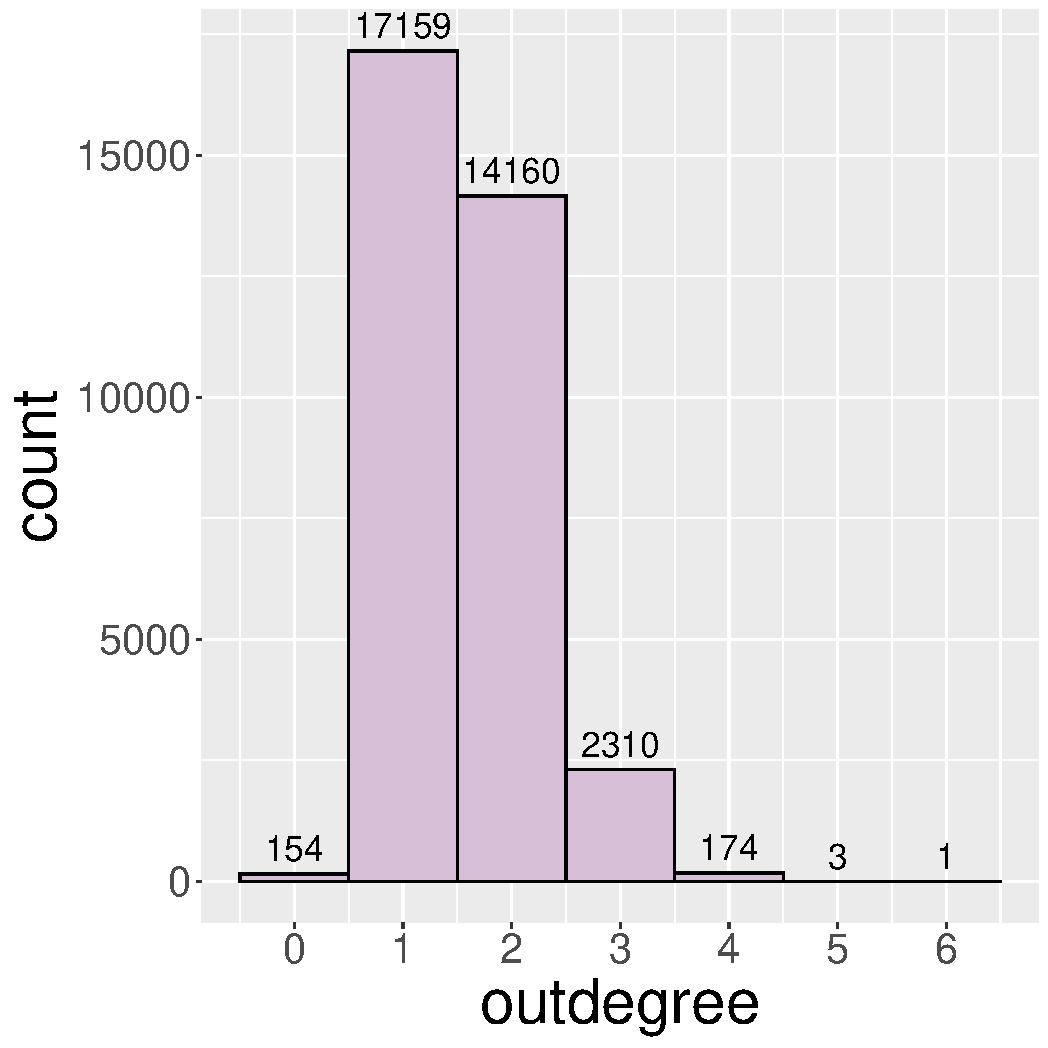
\includegraphics[width=0.4\textwidth]{img/outdegree.pdf}\label{outd_v}}
    \hspace{0em}
    \subfigure[Indegree distribution (edges).]{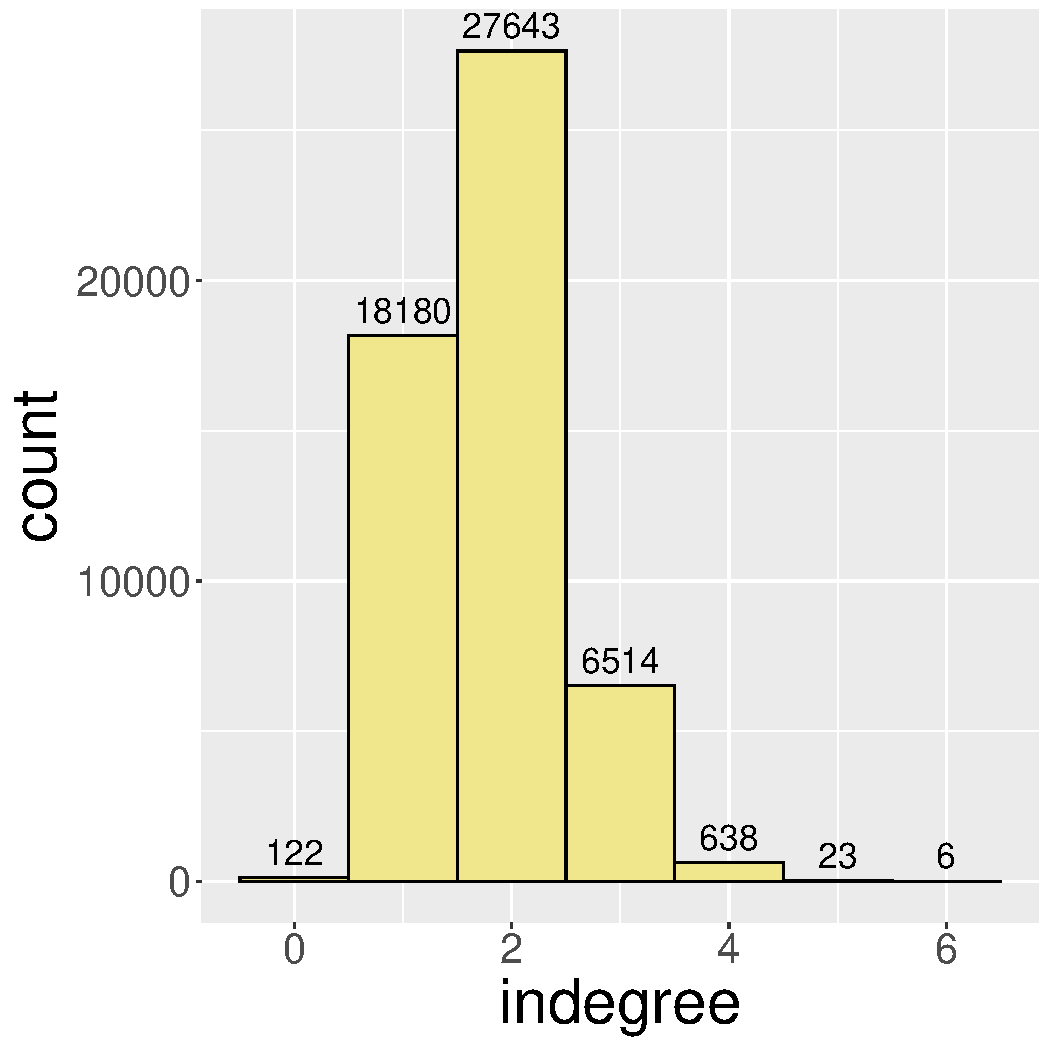
\includegraphics[width=0.4\textwidth]{img/edge-indegree.pdf}\label{ind_e}}
    \hspace{0em}
    \subfigure[Outdegree distribution (edges)]{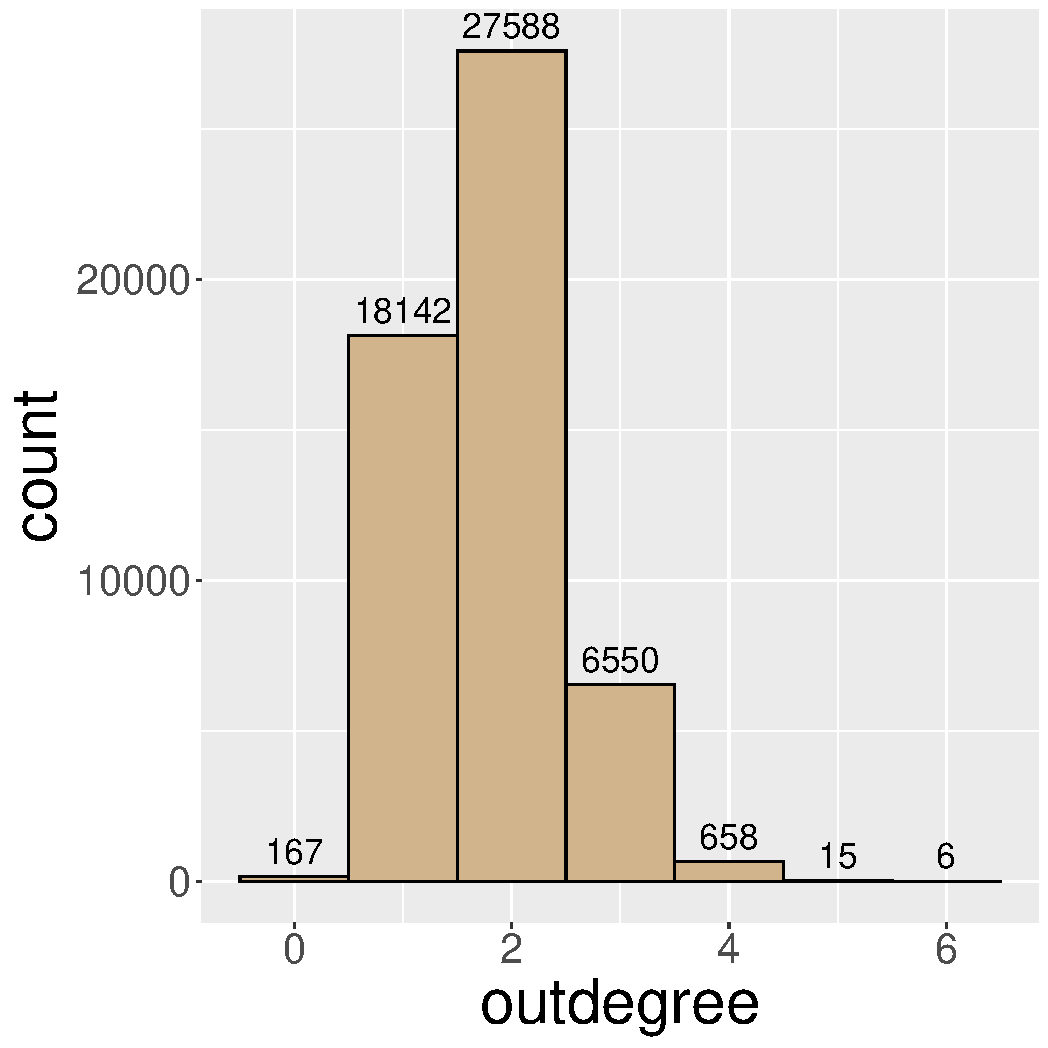
\includegraphics[width=0.4\textwidth]{img/edge-outdegree.pdf}\label{outd_e}}
    \hspace{0em}
    \caption{The degree distribution histograms of the Porto map traffic graph. Source: \cite{traffic-paper}.}
    \label{porto-in-out}
\end{figure}

\begin{figure}[!t]
    \centering
    \subfigure[Distribution of all trajectory points shown in a 2D histogram (number of bins: $80\times80$).]{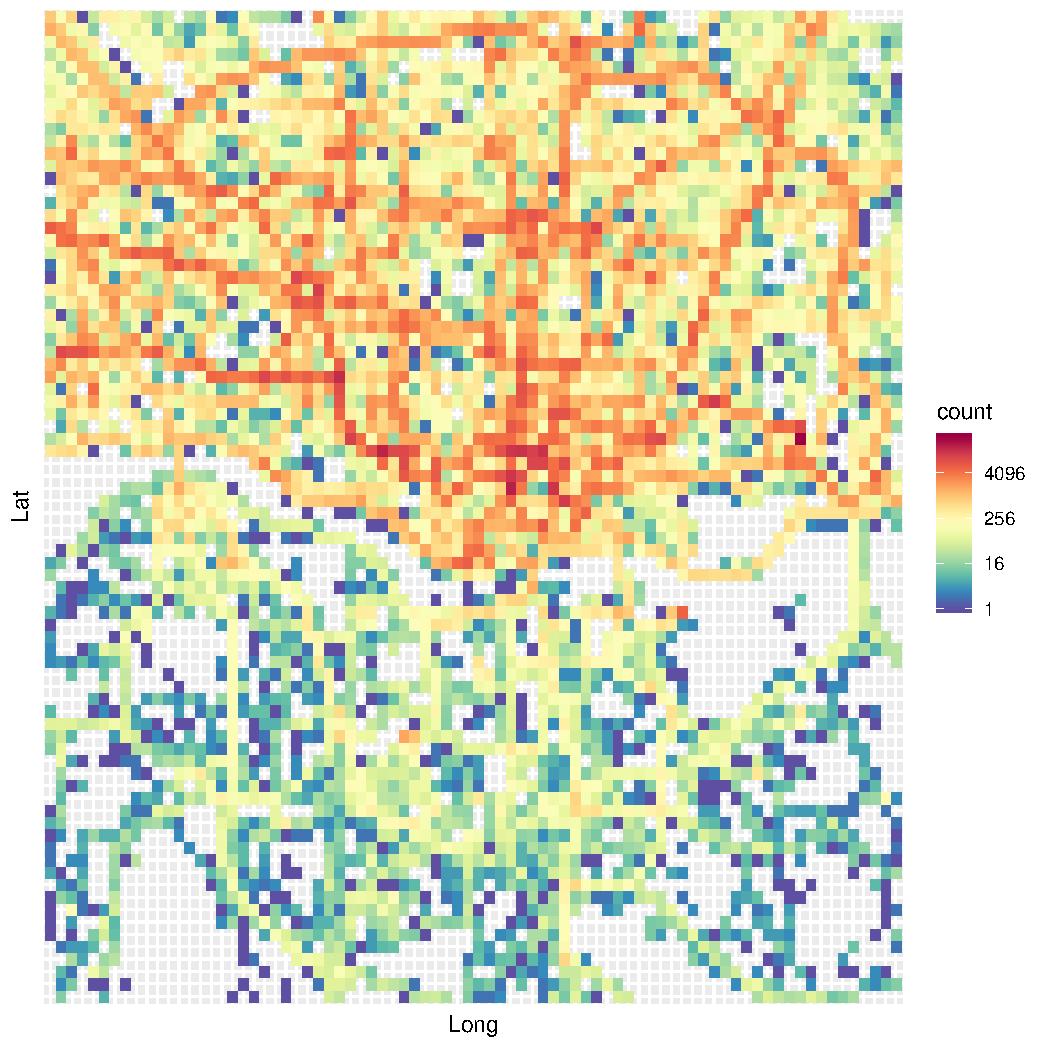
\includegraphics[width=0.4\textwidth]{img/pkdd15_subset_all_80x80.pdf}\label{tr_points_all}}
    \hfill
    \subfigure[Difference of trajectory starting and endpoints shown in a 2D histogram (number of bins: $80\times80$). The color of each bin represents the number of trajectories starting points minus the number of trajectory endpoints that fall in that bin.]{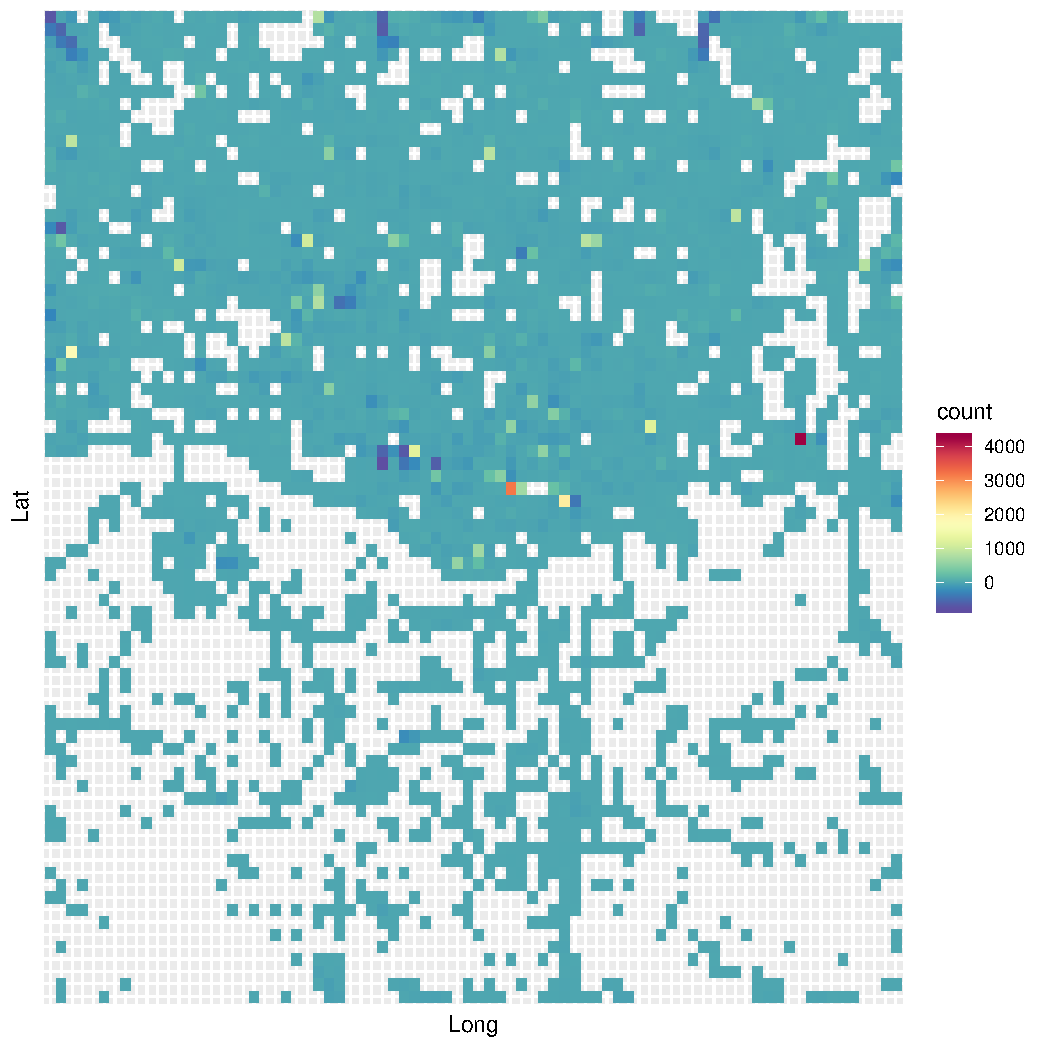
\includegraphics[width=0.4\textwidth]{img/pkdd15_subset_start_minus_end_80x80.pdf}\label{tr_points_start}}
    \hfill
    \subfigure[Histogram of the difference of trajectory starting and endpoints.]{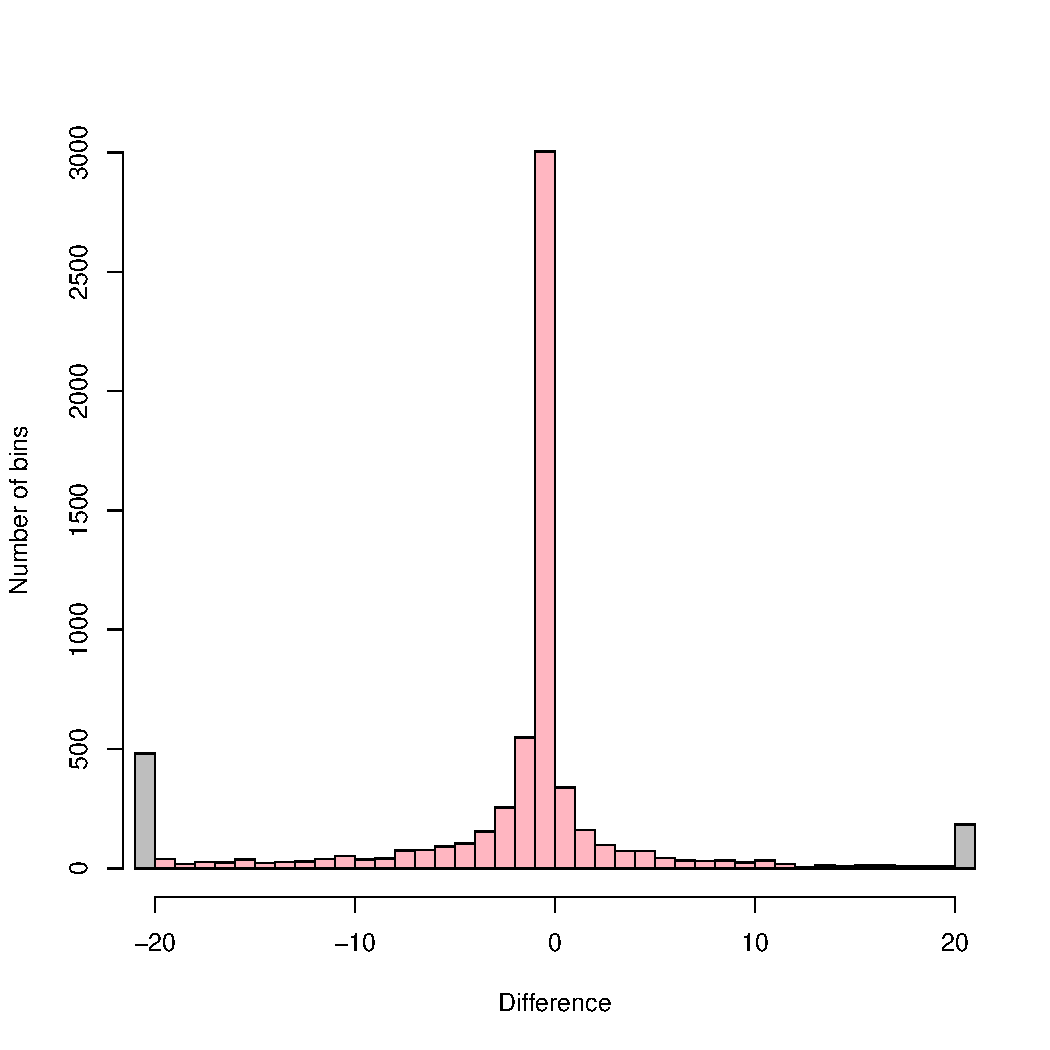
\includegraphics[width=0.4\textwidth]{img/pkdd15_subset_start_minus_end_80x80_hist.pdf}\label{tr_points_end}}
    \caption{Distribution of trajectory points of the filtered dataset. Source: \cite{traffic-paper}.}
    \label{ttp-points}
\end{figure}

\section{Implementation details}

In this section, we present the implementation details of the model in the OOCWC and in some other related software.

As a first step, we have created an R script for the filtering of the Taxi Trajectory Prediction dataset and a Python script for the creation of the Markov kernel from the filtered dataset. The preprocessing scripts open the dataset and select the points according to the limitations described in section \ref{public-dataset}. Then, it saves these points in a new file.\footnote{see \cite[/model-sources/Preprocessing]{csts-repo}} The Python scripts first open the map database with the \texttt{WayNodeHandler} class and build a NetworkX graph by selecting the nodes that are relevant. After that, it converts every point (GPS coordinates) to an OSM node with the \texttt{matching\_thread} function. This function is highly resource demanding, so we implemented it as a multi-process function, as shown in source \ref{node-conv-py} (some lines are omitted for brevity). One can see that we initiate this function as up to 6 distinct processes, one for each trajectory.\footnote{see \cite[/model-sources/Markovkernel]{csts-repo}}

\begin{lstlisting}[language=Python,caption=Multi-process processing of node conversion., label=node-conv-py, escapechar={|}]
with open('pkdd15-subset-bbox-train.csv') as csvfile:
    reader = csv.DictReader(csvfile)
    for row in reader:
        line = row['polyline'].translate(None,'[]')
        coordinates = line.split(',')
        
        threadd = multiprocessing.Process(target=matching_thread,args=(coordinates,))
        threadd.daemon = True
        threadd.start()
        
        count = count + 1
        if(count%6 == 0):
            threadd.join()
        ...
trajectories = np.asarray(trajectories)
\end{lstlisting}

Since most trajectories are not complete in a sense that they are not matched with the OSM graph, i.e., the sampling of trajectories differs from the OSM graph, we interpolated every trajectory to obtain a neighbor-to-neighbor path on the graph, see the \texttt{interpolation} function. Finally, we create the Markov kernel as defined in section \ref{model-desc}.

Regarding the RCE, we performed several modifications, including:
\begin{itemize}
    \item Extended the OSMReader to read the Markov kernel file.
    \item Extended the shared memory segment in the Smart City Server to handle probability vectors.
    \item Modified the Car entity to work according to the probability vectors.
\end{itemize} 

First, we extended the operation of the OSMReader to be able to handle kernel files. For this we added new command line arguments for the Smart City Server and added some basic file reading functionality to the OSMReader. We open the file and read every vector from the Markov kernel file into the corresponding shared memory segment.

Second, we extended the shared memory segment to handle probability vectors for every node. The relevant memory works as shown in source \ref{shm-osmreader}. The \texttt{AdjacencyList} is a map that consists of (1) the ID of the node (2) a pair that consists of (2a) the list of the IDs of the adjacent nodes and (2b) a list of the transition probabilities to the corresponding adjacent nodes. We read the transition probabilities from the kernel file to the \texttt{ProbabilityVect} segment. If there is no probability vector for a node, we initialize this vector according to uniform distribution.

\begin{lstlisting}[language=C++,caption=The shared memory segment of a Markov traffic., label=shm-osmreader, escapechar={|}]
typedef std::vector<osmium::unsigned_object_id_type> WayNodesVect;
typedef std::vector<double> ProbabilityVect;
typedef std::pair<WayNodesVect, ProbabilityVect> WayNodesProbability;
typedef std::map<osmium::unsigned_object_id_type, WayNodesProbability> AdjacencyList;
\end{lstlisting}

Finally, we had to modify the basic operation of the simulation algorithm. In the original implementation, the cars are moving on the map according to random walk or ant simulation. Now, a car selects the next node based on the probability vector of the current node. For this, we use the pseudo-random number generation engine from the Boost Random library\footnote{\url{https://www.boost.org/doc/libs/1_58_0/doc/html/boost_random.html}} that is based on the method presented in paper \cite{Matsumoto}. The node selection procedure is shown in Source \ref{car-markov}.

\begin{lstlisting}[language=C++,caption=Operation of the car entity in a Markov traffic simulation., label=car-markov, escapechar={|}]
  double_vector prv = traffic.getProbabilityVector(next_m_from);

  boost::random::mt19937 gen;
  boost::random::discrete_distribution<> dist(prv);
  gen.seed(static_cast<unsigned int>(std::time(0)));

  osmium::unsigned_object_id_type next_m_to = dist(gen);
\end{lstlisting}

We illustrate the operation of the implementation of the simulation algorithm with an intersection. Observe Fig.~\ref{mapexample} and Table \ref{transitions_example}. This intersection has the OSM ID 1110673569 and GPS coordinates 41.1752185, -8.6231927. From the trajectory dataset, we calculated 1,649 total transitions on this intersection, i.e., 1,649 trajectories go through this intersection. The transitions to the neighbor nodes can be observed in Table \ref{transitions_example}. It is important to note that the actual transition probability (TP) is not the same as the frequency (or the maximum likelihood) based TP. The actual TP, which is the WLS based TP, is given by the Markov kernel file, and has been derived by our method. This simple example shows clearly the difference between the two methods.

\begin{table}[!h]
\centering
\caption{Transitions of intersection 1110673569.}
\label{transitions_example}
\vspace{.5cm} 
\begin{tabular}{c |r r r}
Neighbor node    & \# of transitions & ML based TP & WLS based TP  \\ \hline
1471136241          & 1449  & 0.879 & 0.6    \\ 
1110673512          & 170  & 0.103   & 0.382   \\ 
1837918561          & 30  & 0.018   & 0.018  \\ 
\hline
Sum & 1649 & 1 & 1
\end{tabular}
\end{table}

\begin{figure}[!t]
    \centering
    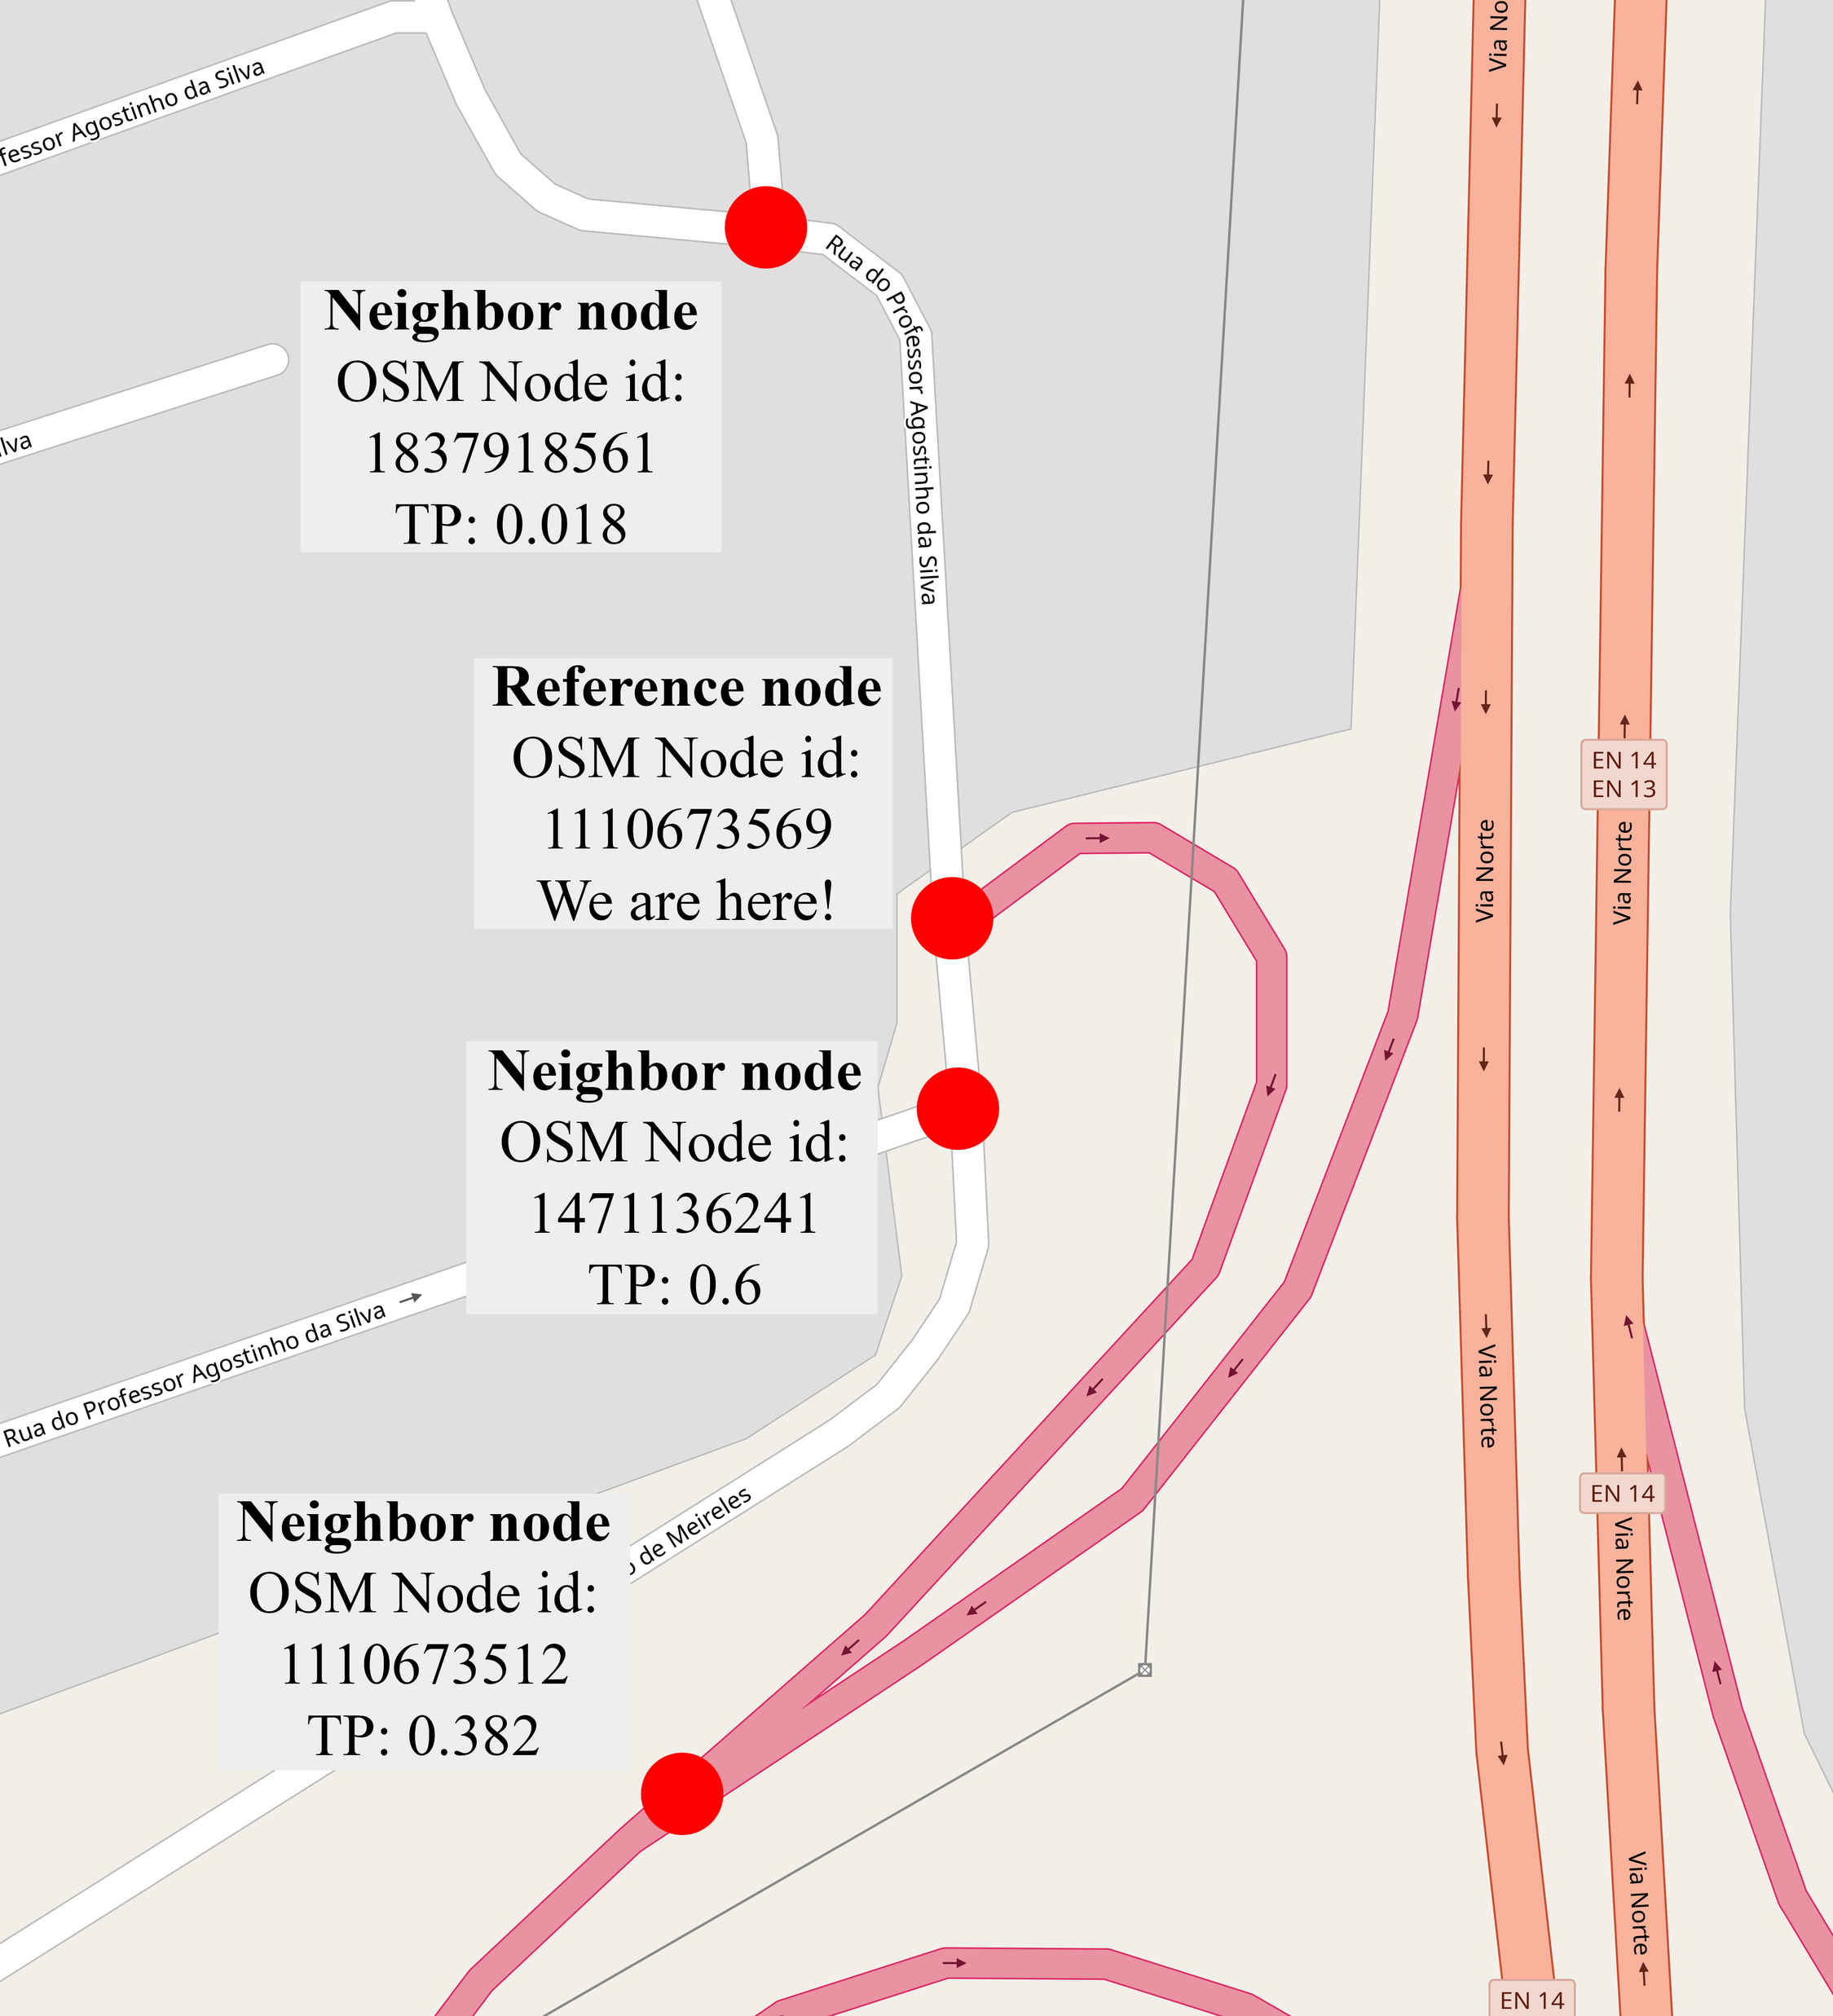
\includegraphics[width=.65\textwidth]{img/map_example_new.jpg}
    \caption{A visual explanation of transitions of intersection 1110673569. TP means transition probability, red dots indicate nodes. Source: \cite{traffic-paper}. (Base map and data from OpenStreetMap and OpenStreetMap Foundation. \copyright OpenStreetMap contributors, annotated by the authors.)}
    \label{mapexample}
\end{figure}

\section{Evaluation of the proposed model}
\label{evaluation}

To evaluate the performance of the proposed WLS estimation method by comparing it to the traditional ML one, a simulation study was conducted at different sample sizes. The trajectories in the Porto dataset have a relatively short length (around 41 points) compared to the size of the traffic graph (around 34K vertex), so, in the simulations, we somewhat mimic this by keeping the length of trajectories low and the number of trajectories high. The absolute bias of an investigated estimator $\widehat{Q}$ for the two-dimensional stationary distribution $Q$ as a parameter is defined by $\|\widehat{Q} -Q\|_G$. The empirical absolute bias and its standard error (SE) correspond to the mean and standard deviation of absolute biases in 100 replications, respectively. All simulations were carried out using the PyDTMC library\footnote{\url{https://pypi.org/project/PyDTMC/}}.

First, we evaluated the model on the small road network in Fig.~\ref{graph-example-1} using the kernel of Fig.~\ref{pi_graph}, see also the Appendix for a toy example. The parameters were $k=100,200,500,$ and $1000$ numbers of trajectories with $n=3,5$ and $10$ lengths. The results can be seen in Table \ref{simulation_small}. The absolute bias and its standard error do not depend on $n$ and, as expected, both are decreasing as $k$ is increasing for the ML and the WLS estimation methods, as well. For small and medium $k$, the two methods perform similarly, but if $k$ gets higher, the ML estimator outperforms the WLS one a bit. This phenomenon could be due to the asymptotic optimality of the ML estimator because the parameter $k$ is large enough (1000 trajectories) compared to the size of the road graph (5 nodes).

For the second evaluation, we tried to mimic a real traffic network, so we exported a strongly connected subgraph from the OSM map of Porto. This graph contains 1,056 vertices and has somewhat similar properties than a large traffic graph, i.e.~can be considered a sparse graph and has the same indegree and outdegree distribution. The GPS coordinates of the bounding box are W8.6137, W8.5991, N41.1573, N41.1437. The entries of Markov kernel were generated randomly, and the simulation parameters were $k=1000,3000$ and $5000$ with $n=3,5$ and $10$. It can be seen clearly in Table \ref{simulation_large} that the absolute bias and the SE is also independent of $n$. However, the performance of the ML and the WLS estimator show significant difference as we change the parameter $k$. On the one hand, the absolute bias of the ML estimator is decreasing with higher $k$, but it is constant for the WLS one. On the other hand, the WLS estimator is better with lower $k$, but worse with higher $k$ than the ML estimator. In real traffic settings, lower $k$'s are more typical, so this simulation corroborates the superiority of WLS method based on two-dimensional stationary distribution against the traditional maximum likelihood. Finally, the scale of the SE's of the WLS estimator shows that it is more stable in this scenario.

\begin{table}[!b]
\centering
\caption{Simulation results, absolute bias and SE (inside parenthesis), for the Markov kernel in Fig.~\ref{pi_graph} on the road network in Fig.~\ref{graph-example-1}. ($k$ - number, $n$ - length of trajectories)}
\label{simulation_small} 
\begin{tabular}{c c | c c}
k & n & ML & WLS  \\ \hline
100 & 3 & 0.034 (0.0103) & 0.034 (0.0109)\\ 
100 & 5 & 0.035 (0.0106) & 0.034 (0.0103)\\ 
100 & 10 & 0.033 (0.0095) & 0.033 (0.0094)\\ 
200 & 3 & 0.024 (0.0066) & 0.026 (0.0066)\\ 
200 & 5 & 0.023 (0.0064) & 0.024 (0.0067)\\ 
200 & 10 & 0.024 (0.0071) & 0.025 (0.0070)\\ 
500 & 3 & 0.015 (0.0046) & 0.017 (0.0049)\\
500 & 5 & 0.015 (0.0041) & 0.017 (0.0049)\\
500 & 10 & 0.016 (0.0047) & 0.017 (0.0049)\\
1000 & 3 & 0.010 (0.0032) & 0.013 (0.0041)\\
1000 & 5 & 0.011 (0.0034) & 0.015 (0.0044)\\
1000 & 10 & 0.010 (0.0030) & 0.014 (0.0040)
\\
\hline
\end{tabular}
\end{table}

\begin{table}[!h]
\centering
\caption{Simulation results, absolute bias and SE (inside parenthesis), for a part of Porto's map with 1000 vertices. ($k$ - number, $n$ - length of trajectories)}
\label{simulation_large} 
\begin{tabular}{c c | c c}
k & n & ML & WLS  \\ \hline
1000 & 3 & 0.166 (0.0559) & 0.025 (0.0007) \\
1000 & 5 & 0.184 (0.1214) & 0.025 (0.0007) \\
1000 & 10 & 0.169 (0.0938) & 0.025 (0.0008) \\
3000 & 3 & 0.064 (0.1725) & 0.023 (0.0005) \\
3000 & 5 & 0.070 (0.1665) & 0.023 (0.0005) \\
3000 & 10 & 0.063 (0.1705) & 0.023 (0.0005) \\
5000 & 3 & 0.016 (0.0150) & 0.023 (0.0004) \\
5000 & 5 & 0.014 (0.0055) & 0.023 (0.0004) \\
5000 & 10 & 0.014 (0.0126) & 0.023 (0.0003) \\
\hline
\end{tabular}
\end{table}

Finally, we tested the simulation model in the OOCWC. The initialization phase of the simulation adds traffic units to the vertices of the simulation graph. There exists two ways to do this, one is following a prescribed distribution (e.g.~uniform), the other is following measured data. In this test setup, we initialized simulations with fictional data. We put units only to the streets Rua de Antero de Quental, Rua da Constitui\c{c}\~ao and Rua da Boavista (25.6\%, 51.4\%, 23\% of the cars, respectively), i.e., the simulation starts from the traffic configuration which is concentrated on three nodes of the road graph. We run simulations with $k=5,000, 10,000, 20,000, 30,000$ and $50,000$ units. The simulation starts when all simulation units are added to the map. Fig.~\ref{cardist} shows the change of the distribution of cars during the simulation.

\begin{figure*}[!h]
    \centering
    \subfigure[Initial step (10k cars).]{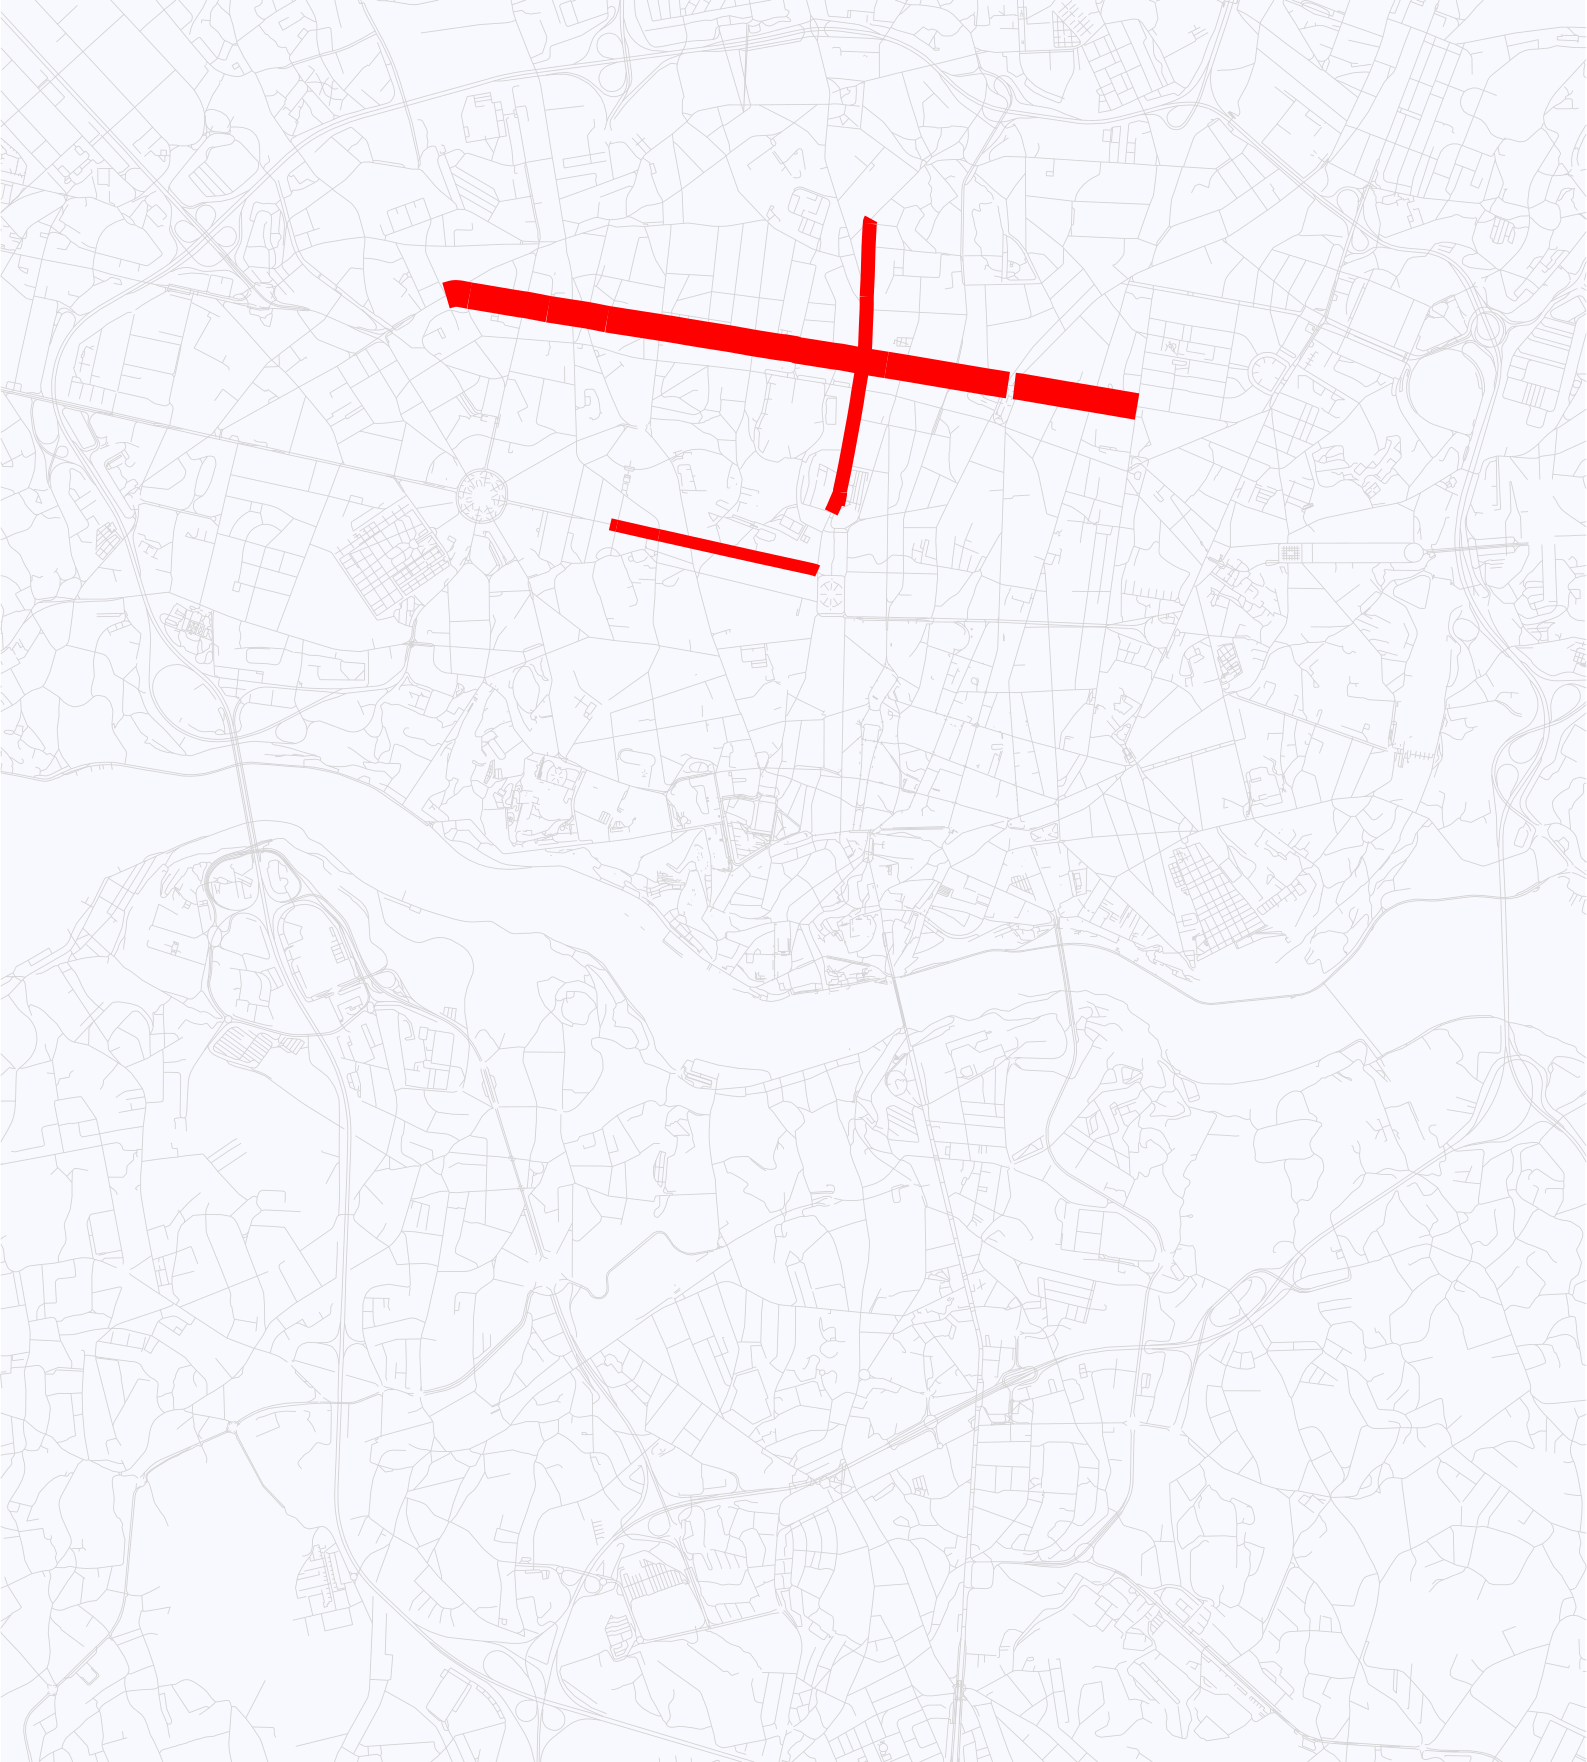
\includegraphics[width=0.32\textwidth]{img/DIST_10k_1min_1.png}\label{simul_init_10}}
    \hspace{0em}
    \subfigure[After 30 mins (10k cars).]{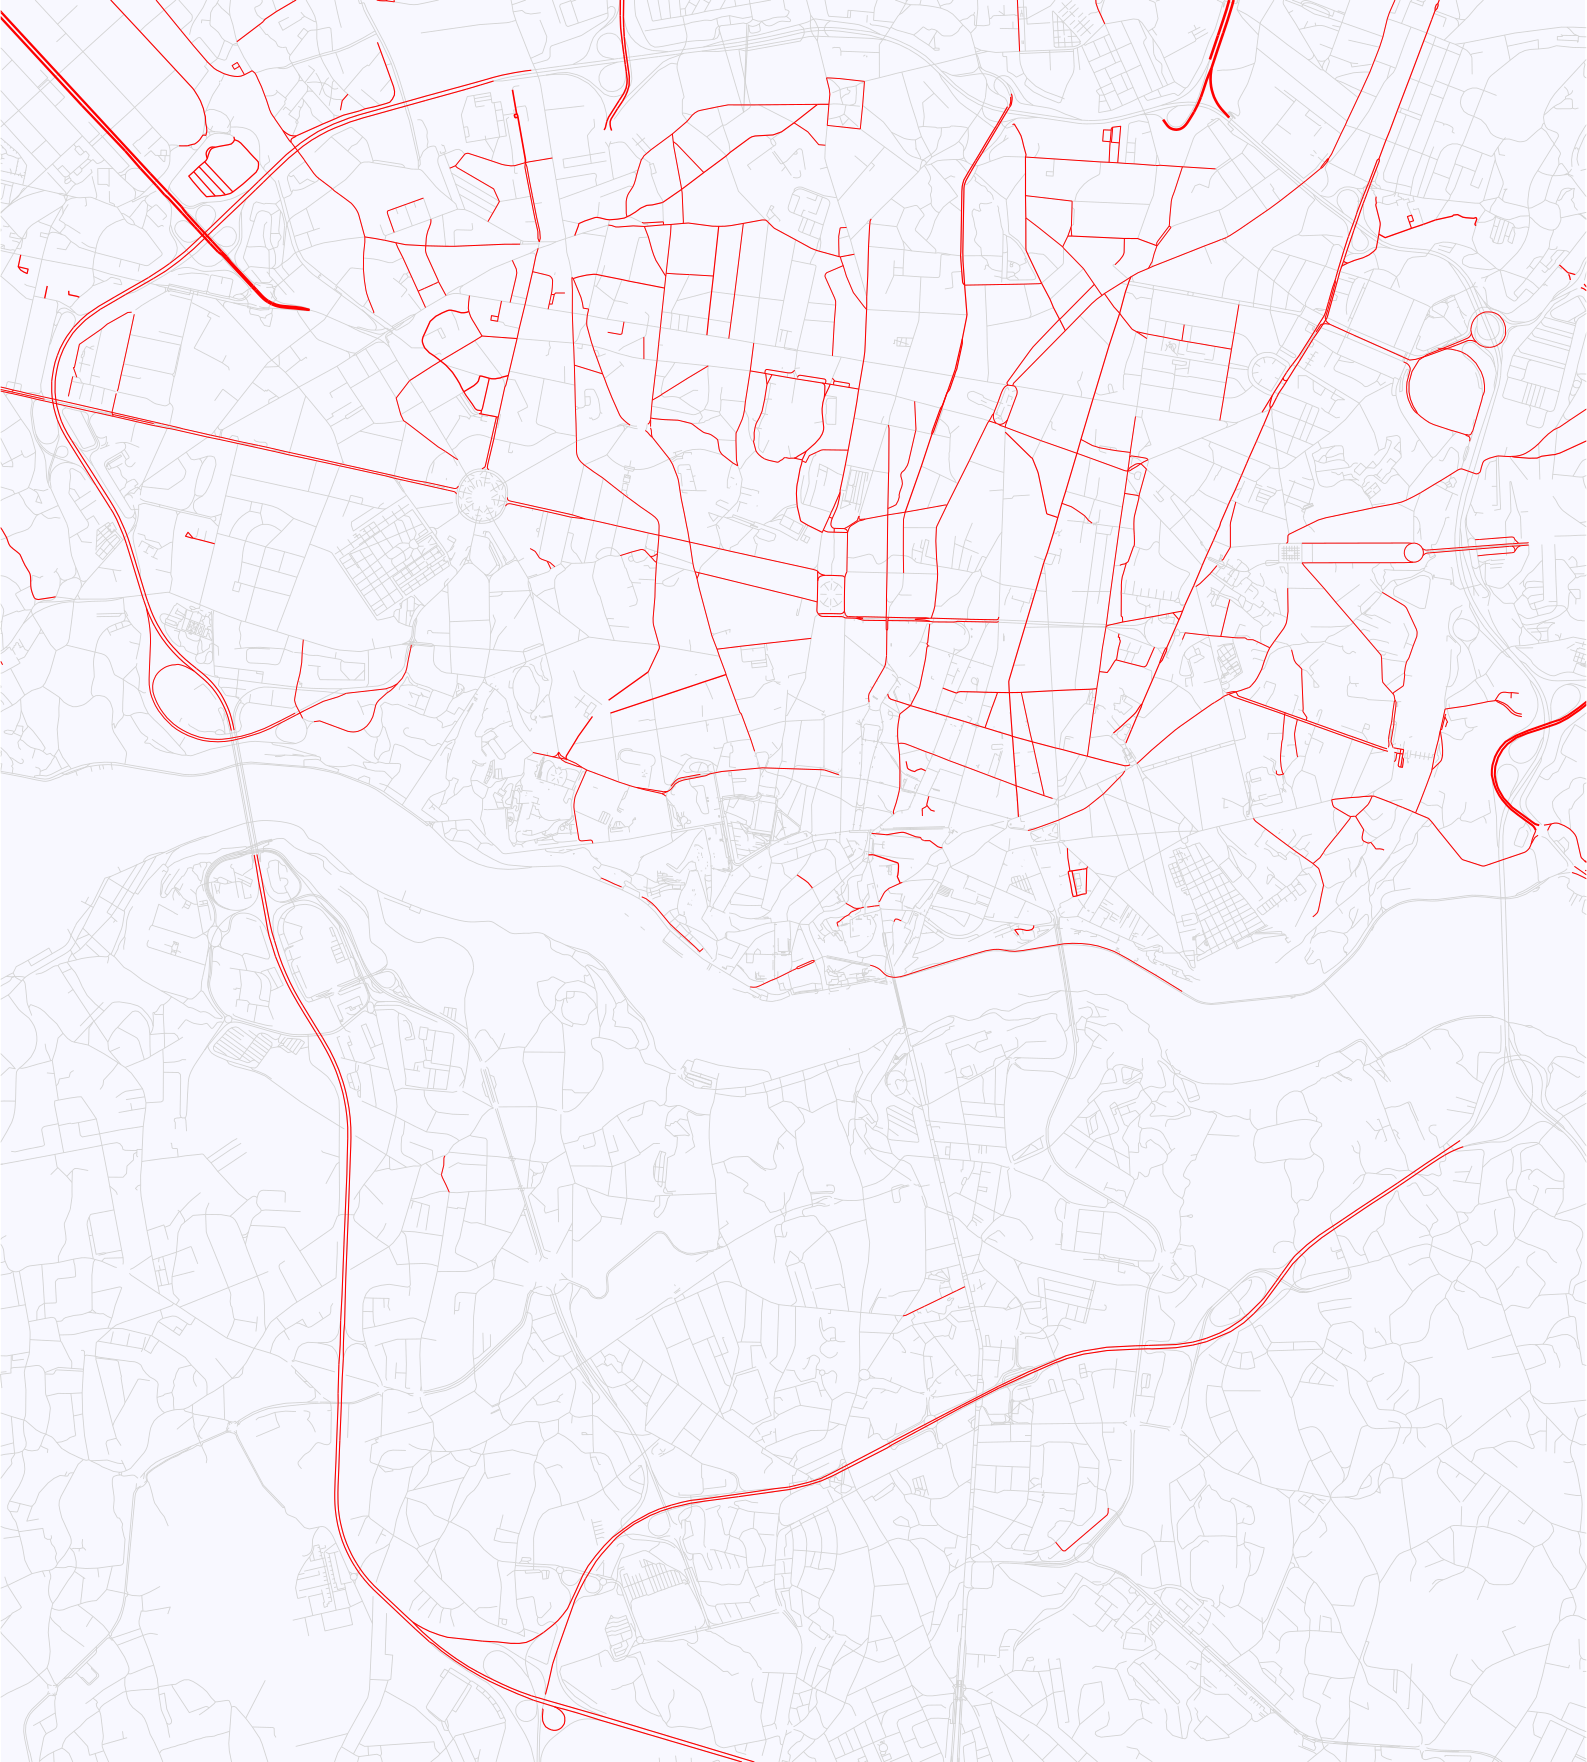
\includegraphics[width=0.32\textwidth]{img/DIST_10k_1min_31.png}\label{simul_30_10}}
    \hspace{0em}
    \subfigure[After 60 mins (10k cars).]{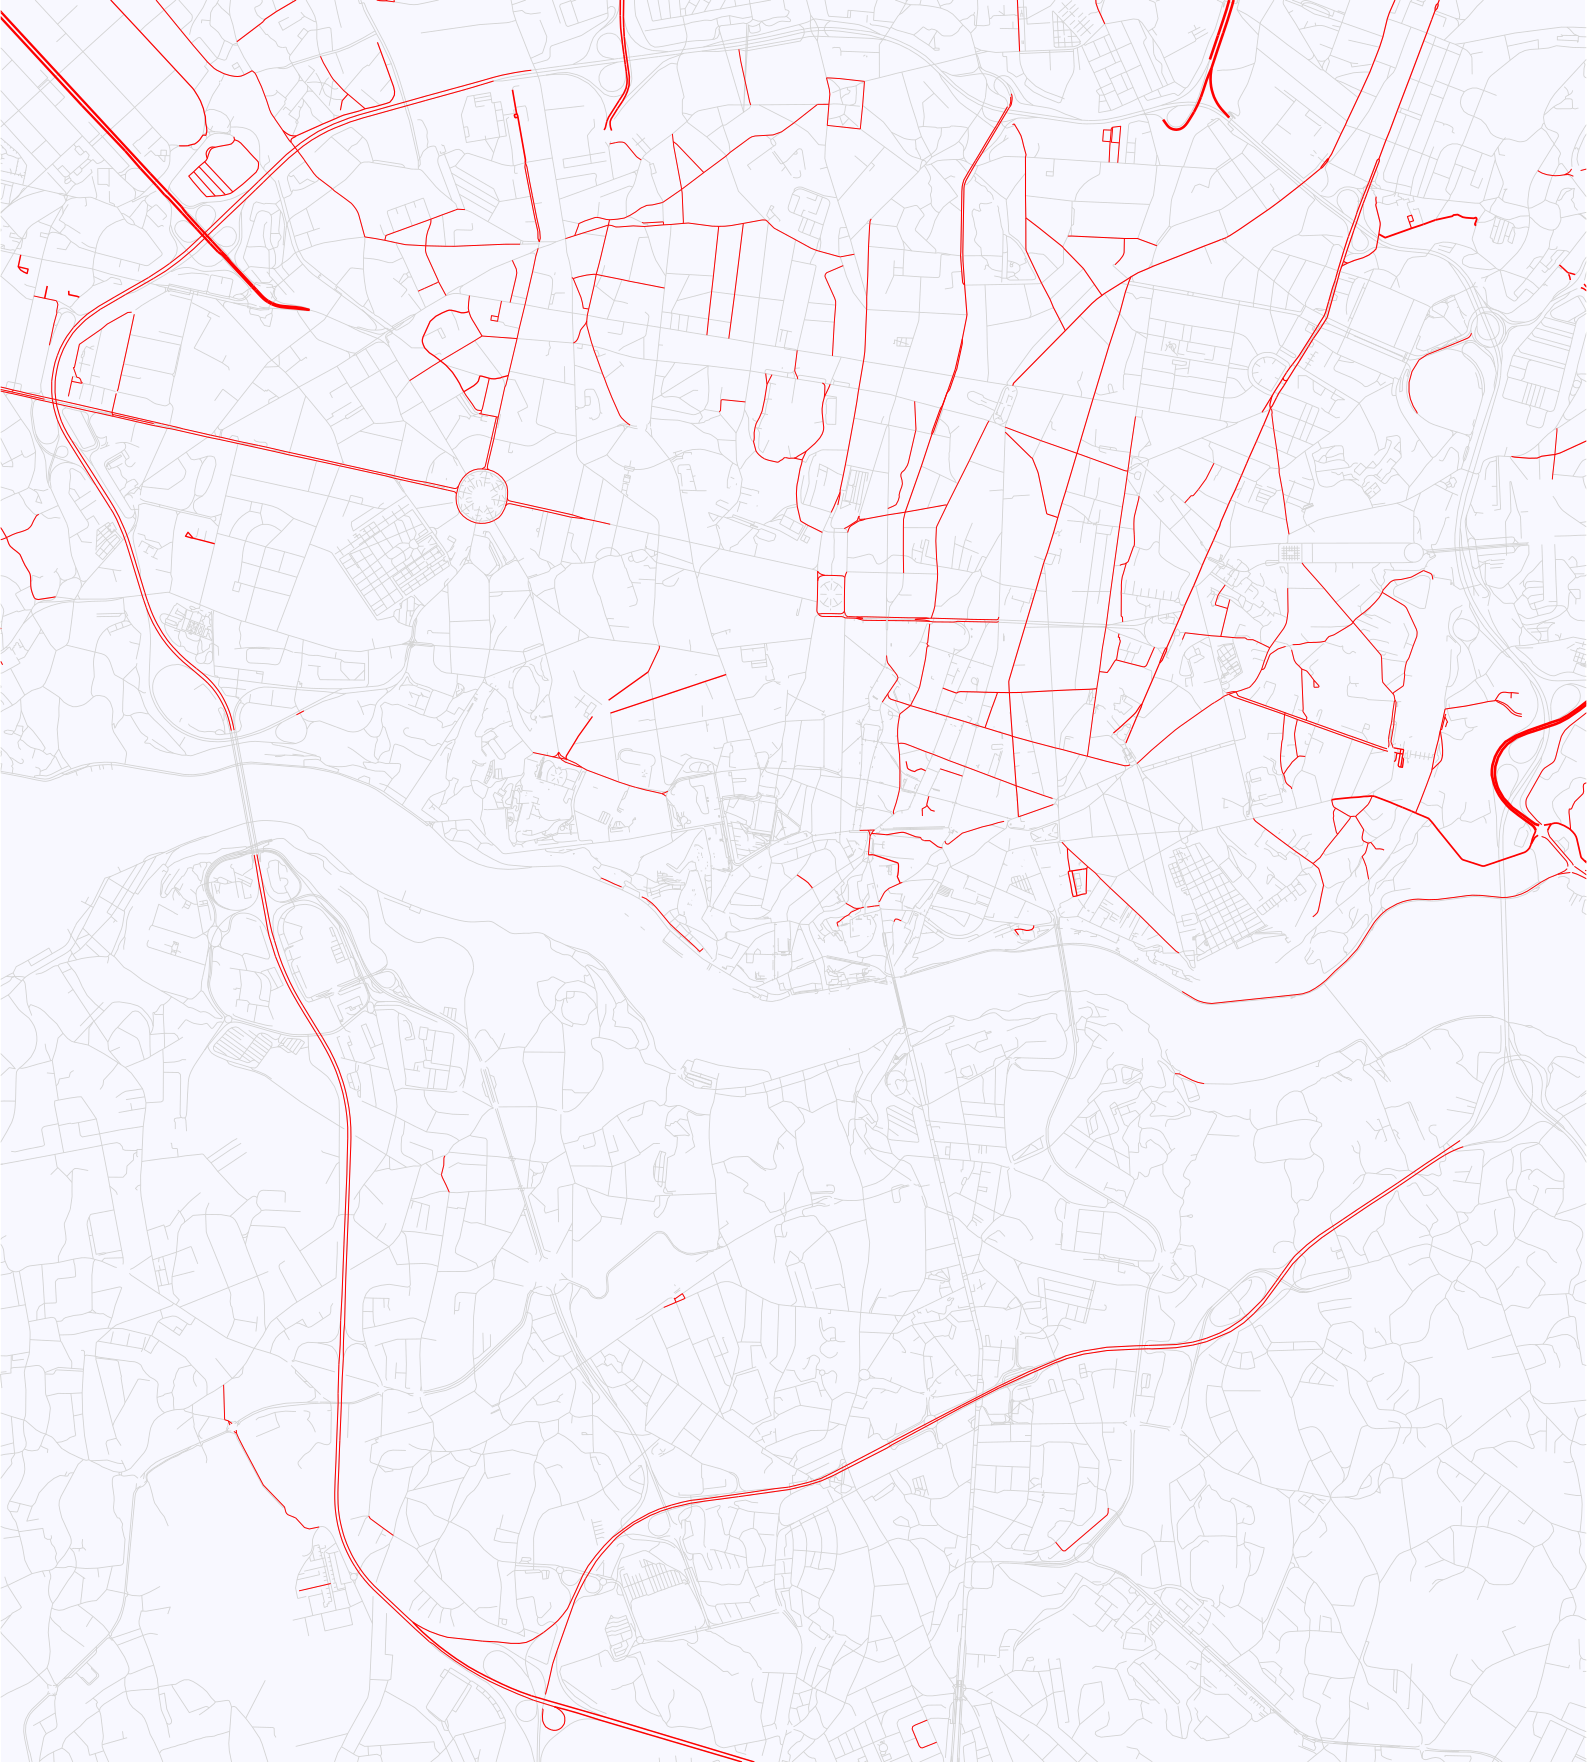
\includegraphics[width=0.32\textwidth]{img/DIST_10k_1min_61.png}\label{simul_60_10}}
    \hspace{0em}
    \\
    \subfigure[Initial step (20k cars).]{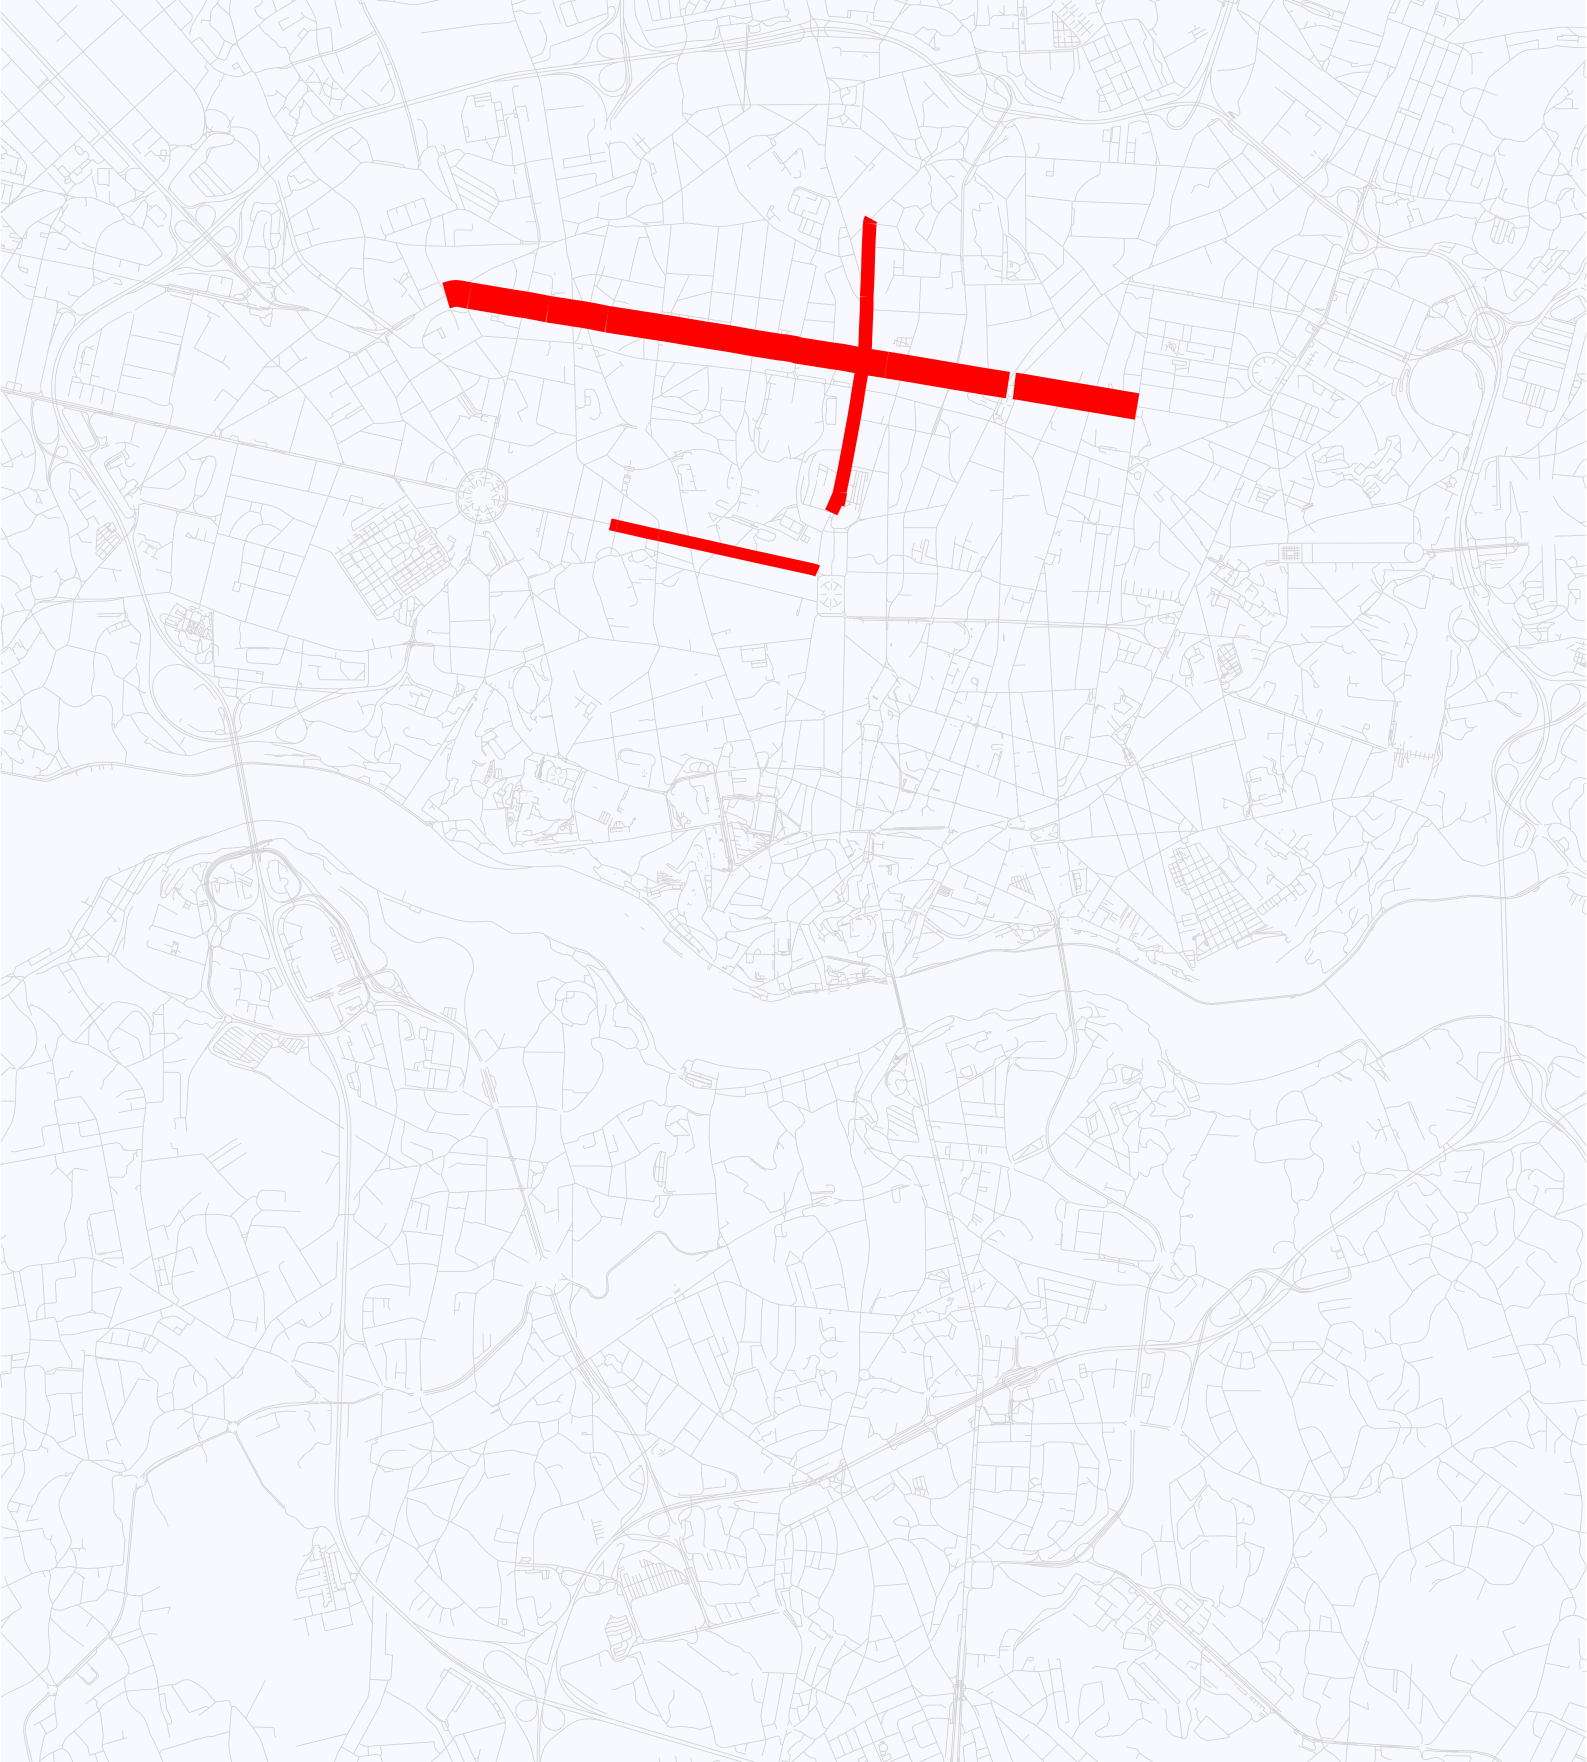
\includegraphics[width=0.32\textwidth]{img/DIST_20k_1min_1.png}\label{simul_init_20}}
    \hspace{0em}
    \subfigure[After 30 mins (20k cars).]{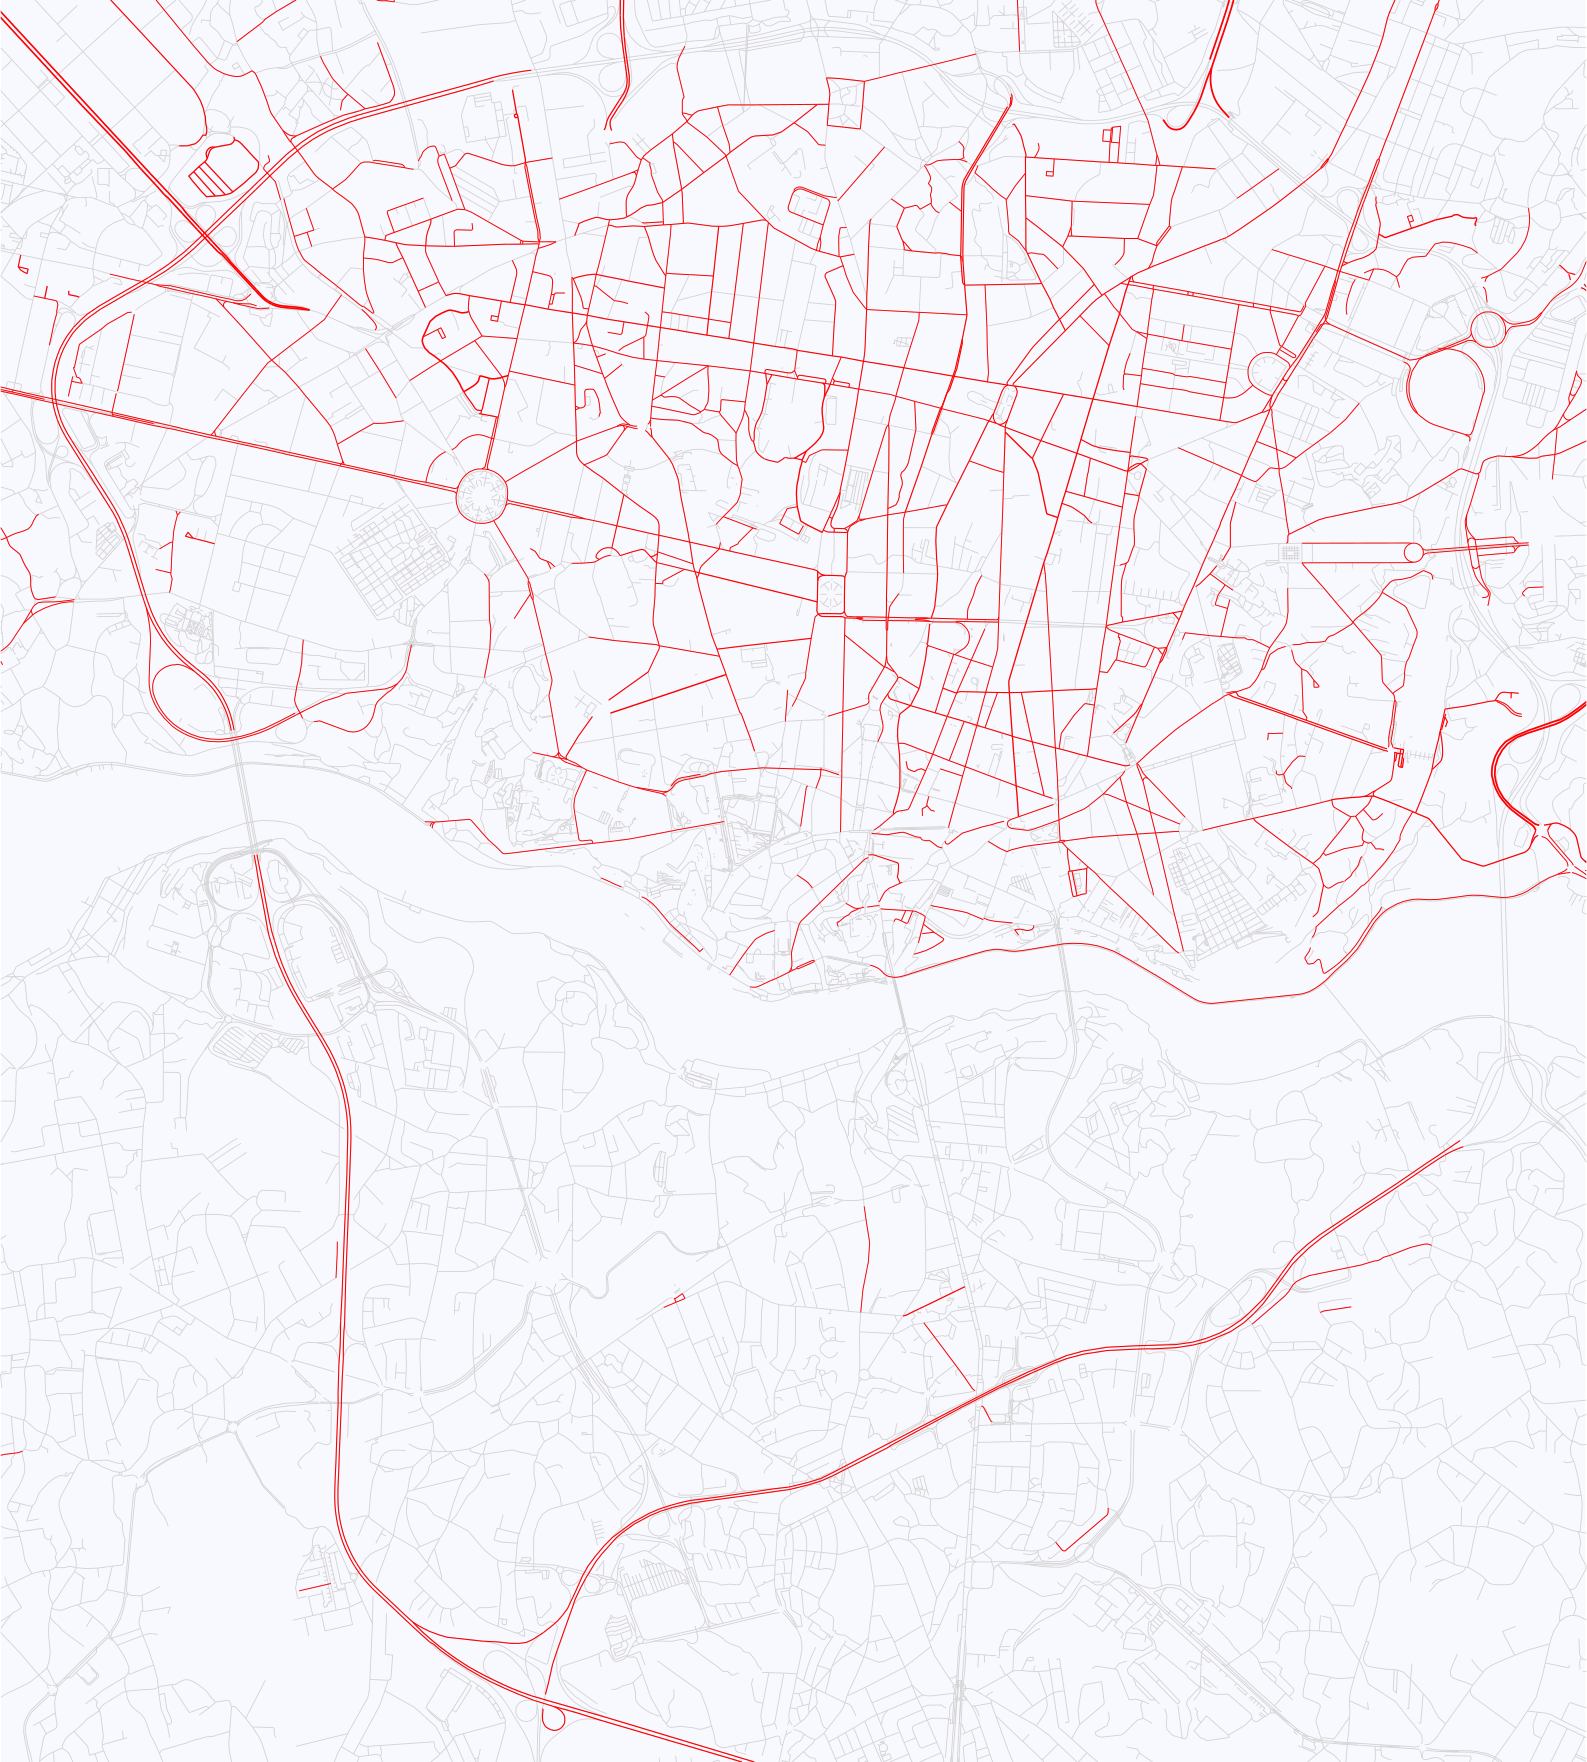
\includegraphics[width=0.32\textwidth]{img/DIST_20k_1min_31.png}\label{simul_30_20}}
    \hspace{0em}
    \subfigure[After 60 mins (20k cars).]{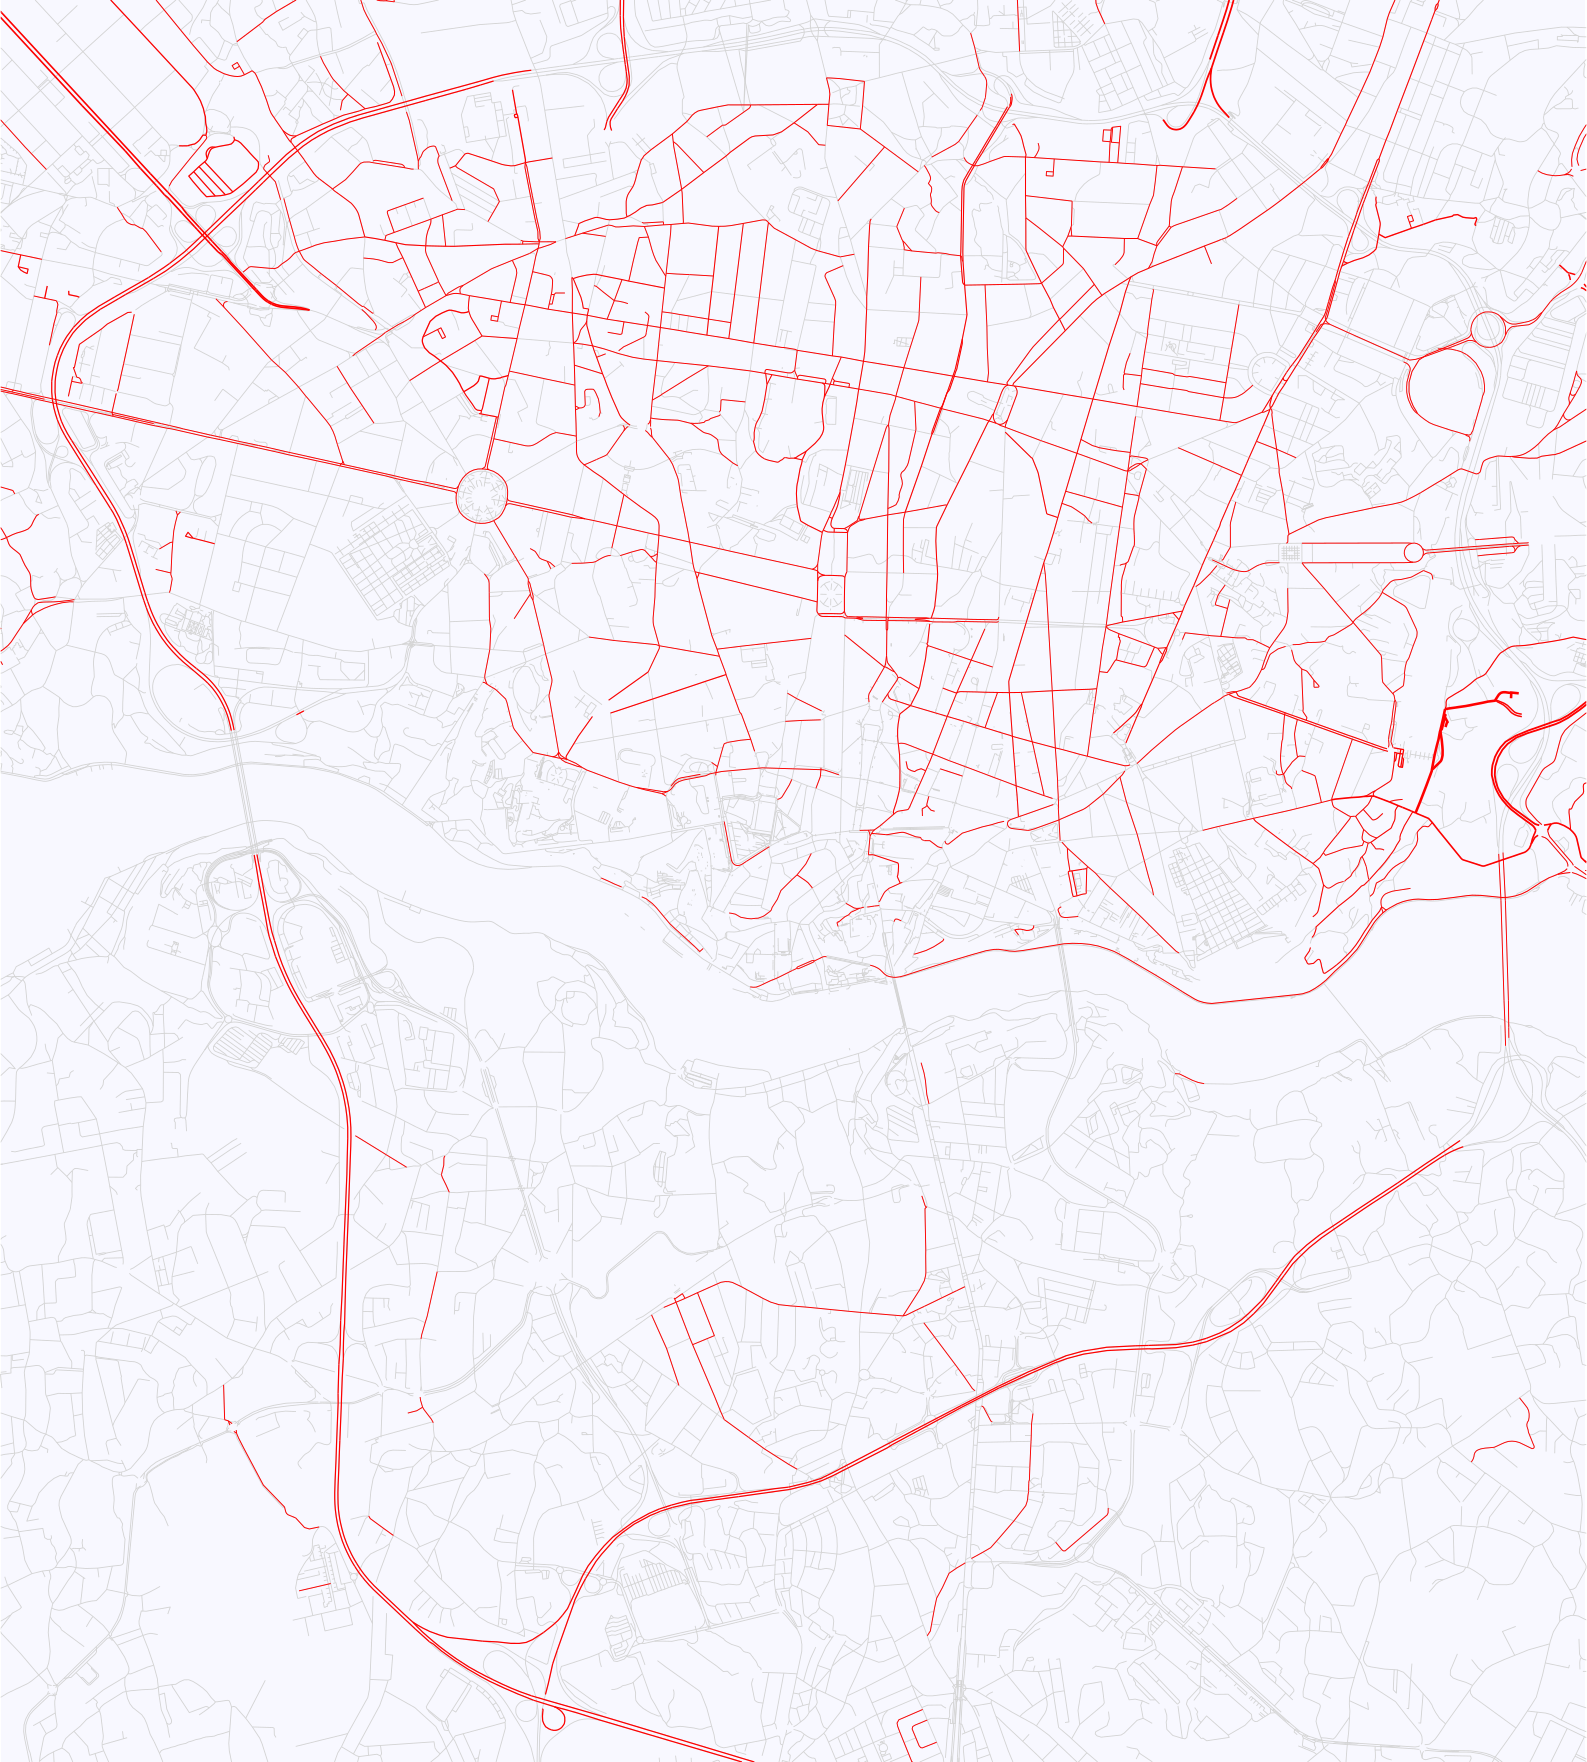
\includegraphics[width=0.32\textwidth]{img/DIST_20k_1min_61.png}\label{simul_60_20}}
    \hspace{0em}
    \caption{The change of the distribution of cars during the simulation (10,000 and 20,000 cars). The thickness of the street is proportionate with the number of cars on the street. Source: \cite{traffic-paper}.}
    \label{cardist}
\end{figure*}

We can extract and calculate the number of cars by street in every minute from a file produced by the RCE, so we can observe the change of distribution of the cars. Comparing it with the previously calculated stationary distribution (see Fig.~\ref{porto_stat_dist}), it shows us the operation of the implementation of the model. Please note the similarity between Fig.~\ref{porto_stat_dist} and Fig.~\ref{tr_points_all}. The ticker line on Fig.~\ref{porto_stat_dist} corresponds to increasingly hot color on Fig.~\ref{tr_points_all}.

\begin{figure}[!b]
    \centering
    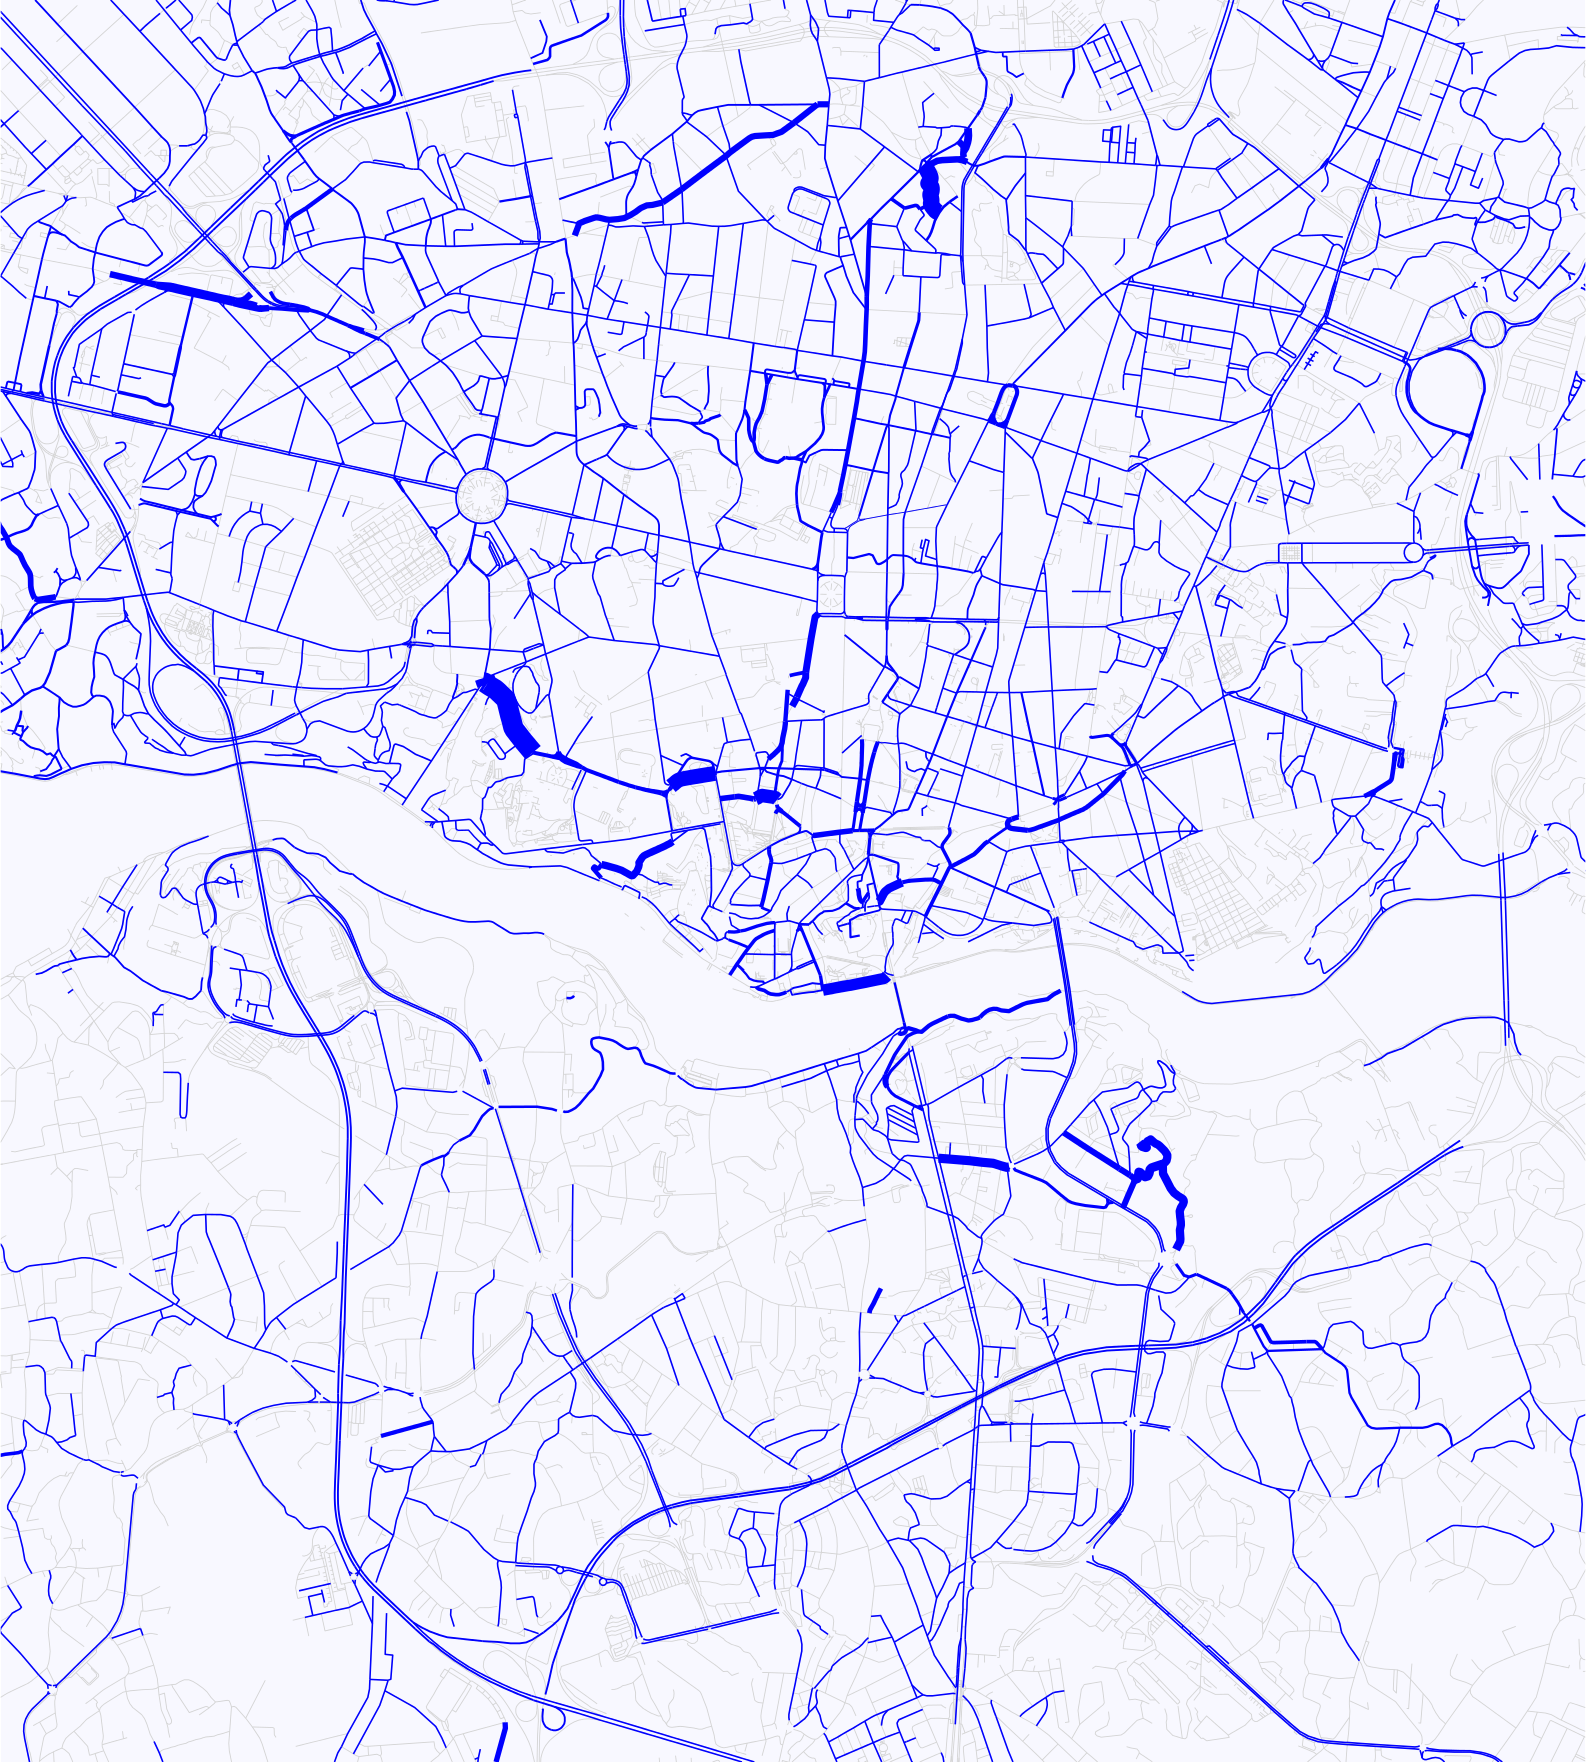
\includegraphics[width=.6\textwidth]{img/porto_stat_dist.png}
    \caption{The two-dimensional stationary distribution of cars in Porto based on the TTP dataset. Source: \cite{traffic-paper}.}
    \label{porto_stat_dist}
\end{figure}

We applied the Pearson's chi-squared test to compare the actual distribution of the cars minute-by-minute with the stationary distribution. We expect, based on the ergodicity of Markov traffic, see section 2.3 of paper \cite{traffic-paper}, that during the simulation, independently from the initial distribution, within a certain time period, the distribution of the cars become close to the previously calculated stationary distribution. Fig.~\ref{DIST_chi_sq} shows the test results. We can observe that in the first few minutes the test statistic is high. This means that the distribution of the cars is still far from the previously calculated steady state. However, after a time period, which depends on the number of cars, the test statistic becomes lower and remain the same, thus the distribution becomes steady. One can observe a reasonable phenomenon that it takes more time to reach the steady state with more traffic units. Another notable trend is the case of 5,000 cars, where the line is elevating after reaching the steady-state. This can be caused by the low number of cars. The number of individual streets (named or unnamed, e.g., motorway junctions) is 2,194. 5,000 cars are simply not enough statistically to reach and hold a steady state in this type of simulation.

\begin{figure*}[!t]
    \centering
    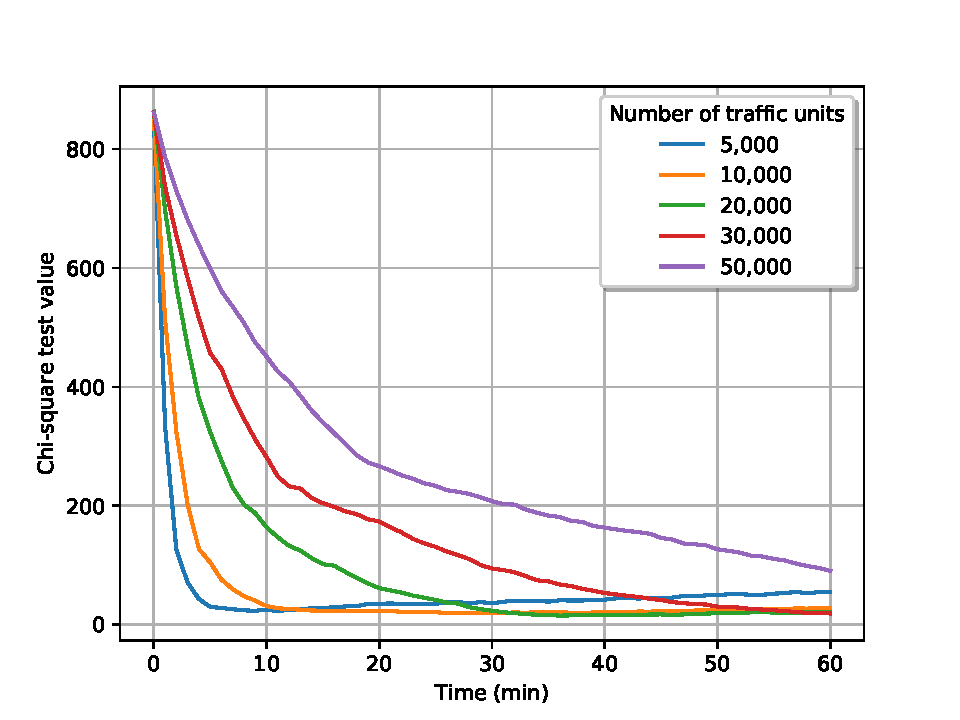
\includegraphics[width=.8\textwidth]{img/DIST.pdf}
    \caption{Chi-square test results. Source: \cite{traffic-paper}.}
    \label{DIST_chi_sq}
\end{figure*}

\section{Conclusions on the simulation algorithms}

In this chapter, we have outlined our mathematical model for traffic simulation that is called \enquote{Markov traffic}. This model is based on tools from graph and Markov chain theories. Our aim was to create a simulation method that is able to keep the distribution of the cars on the traffic graph in a steady state. We have proven that, under general assumptions, the stationary distribution is unique for any Markov transition mechanism on a wide class of road networks.

This transition mechanism and the stationary distribution can be explored from observed trajectories. We have shown a statistical method with which we can create the Markov kernel which is necessary to obtain a Markov traffic. Using this kernel, we can initiate traffic simulations that provide a stationary distribution of the cars on the map. To provide an example for creating this kernel file, we have used a publicly available dataset, namely the Taxi Trajectory Prediction dataset. Our simulation uses OpenStreetMap, from which we extract the traffic graphs.

Finally, we should note a few minor implementation details that can be drawbacks of this model and may have an impact on its overall performance. In smaller graphs, the proposed algorithm and its implementation performs as it is expected, see the evaluation in section \ref{evaluation}. But in the case of large graphs, like our Porto example (33,961 nodes and 53,126 edges) and a very sparse TP matrix (see the degree distribution in Fig.~\ref{porto-in-out}), numerical problems may occur. First, when we calculate the $\widehat{Q}_{\textrm{WLS}}$ estimator and then TP matrix using the method described in section \ref{inference}, we cannot always solve the linear equation of the Lagrange vector in Theorem \ref{main_thm} numerically. We could only use the least square solution for a numerically stable calculation. In some cases, impossible numbers are present in the TP matrix, e.g., for a node, the TP vector is [1.17489, -0.174894]. It is rather interesting that the sum of these \enquote{impossible} TP vectors are 1 all the time, and mostly occurs if the node has a low number of transitions (less than 20). In these cases, we use the frequency-based TP instead. Second, problems can also occur when we calculate the stationary distribution $\bpi$, namely, negative values may be present in the results. We chose to shift every value of $\bpi$ until we get a sum of 1 for $\bpi$ when we calculate the Pearson's Chi-square test. Finally, we should note that the OSM Porto map and the trajectory dataset do not cover each other perfectly, we only know the stationary distribution $\bpi$ for a subgraph of the whole map. The simulation units can traverse the whole OSM map graph, so, it can happen that a traffic unit reaches an edge which is not a part of the subgraph where we know the stationary distribution $\bpi$. When we calculate the Pearson's chi-squared test, we consider only those cars that are present on the subgraph, where the stationary distribution $\bpi$ is known.

The whole project (including the RCE) is available for download.\footnote{see \url{https://github.com/rbesenczi/Crowd-sourced-Traffic-Simulator/blob/master/justine/install.txt}} Some simulation video is available on the YouTube channel of the author.\footnote{see \url{http://bit.ly/2FRpPxL}}

\chapter{Conclusion}
\label{conclusion}

In this thesis, a smart city application is presented. The main function of this application is to simulate traffic in urban environments and to provide a research platform. The main contribution of this thesis is providing two reference implementations for two components of the system.

First, a complex system applied for data collection is presented. It consists of a hardware and a software part. The hardware part is a custom embedded system that can be assembled into cars. Its basic operation is to count cars on a given road segment, aggregate the data, then send data to a central server infrastructure. The Real-Time Traffic Analyzer has been tested and was suitable to conduct measurements and data collection.

Second, a simulation algorithm and its implementation are introduced that can provide a stationary distribution of the cars in a given time period. The proposed algorithm is based on graph theory and a Markov model of probability theory. It is shown that the proposed algorithm can simulate such traffic where the distribution of cars is stationary.

\subsection*{Acknowledgments}
\addcontentsline{toc}{chapter}{Acknowledgments}

\begin{singlespace}
\footnotesize

\noindent
In this thesis, we refer many times for the \enquote{original} implementation of the OOCWC (and its RCE component). This initial version was implemented from scratch by Norbert Bátfai, see its GitHub repository\footnote{\url{https://github.com/nbatfai/robocar-emulator/}}. Every further development outlined in this thesis (and the corresponding papers) has been conducted by me in a fork of his software repository\footnote{\url{https://github.com/rbesenczi/Crowd-sourced-Traffic-Simulator}}.

\noindent
I am grateful to my thesis advisor Márton Ispány for his encouragement and guidance. I am also thankful to the Doctoral School of Informatics of the University of Debrecen for having provided the opportunity to conduct researches and to write my thesis.

\noindent
I would like to thank all the support of the OOCWC and Smart City research groups at the Department of Information Technology. Members are: Márton Ispány, Norbert Bátfai, Péter Jeszenszky and the former students of the High Level Programming Languages courses.

\noindent
I would like to express my special thanks to Norbert Bátfai, because without his exceptional straightforwardness this thesis would not exist. I cannot be grateful enough for Fanny Monori for her invaluable help and endless support.

\noindent
I would like to thank Prof. István Oniga that we could use some of the devices of his research group at the early phase of the development.

\noindent
I could not be grateful enough to my engineer-hacker friends Tamás Katona and Mihály Szilágyi.

\noindent
Most importantly, I would like to thank all the support to my family and my parents.

\noindent
Jelen munka a Nemzeti Tehetség Program, Egyedi fejlesztést biztosító ösztöndíjak NTP-EFÖ-P-15-0187 számú pályázat keretei között készült. A projektet az Emberi Erőforrások Minisztériuma Emberi Erőforrás Támogatáskezelő támogatta.

\noindent
This thesis was supported by the National Talent Programme of Hungary, contract no.: NTP-EFÖ-P-15-0187.

\begin{figure}[h!]
\centering
\subfigure{
\includegraphics[width=1in]{img/emmi}}
\subfigure{
\includegraphics[width=2in]{img/emet}}
\subfigure{
\includegraphics[width=1.5in]{img/ntp}}
\end{figure}

\end{singlespace}


\addcontentsline{toc}{chapter}{Bibliography}
\begin{singlespace}
\footnotesize
\bibliography{thesis}
\end{singlespace}

\chapter*{Appendix}
\addcontentsline{toc}{chapter}{Appendix}

\subsection*{A Toy Example}
\addcontentsline{toc}{section}{A Toy Example}
\label{example}

\begin{figure}
\centering
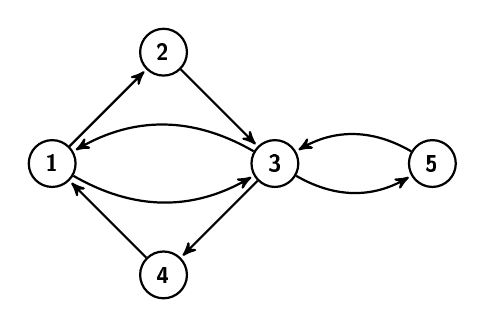
\begin{tikzpicture}[->,>=stealth',shorten >=1pt,auto,node distance=2cm,
                    thick,main node/.style={circle,draw,font=\sffamily\small\bfseries}]
 
  \node[main node] (2) {2};
  \node[main node] (1) [below left of=2] {1};
  \node[main node] (3) [below right of=2] {3};
  \node[main node] (4) [below right of=1] {4};
  \node[main node] (5) [right of=3] {5};  
  \path[every node/.style={font=\sffamily\small}]
    (1) edge node {} (2)
        edge [bend right] node {} (3) 
    (2) edge node {} (3) 
    (3) edge node {} (4)
        edge [bend right] node {} (5)
        edge [bend right] node {} (1)
    (4) edge node {} (1)
    (5) edge [bend right] node {} (3);    
\end{tikzpicture}
\caption{A simple road network.}
\label{toy-graph-example}
\end{figure}

In order to demonstrate the main concepts and methods of section \ref{model-desc} we present a simple toy example.\footnote{For a Python implementation, see: \url{https://github.com/rbesenczi/Crowd-sourced-Traffic-Simulator/blob/master/model-sources/Markovkernel/example_graph_thesis.py}} Consider the road network $G=(V,E)$ on Fig.~\ref{toy-graph-example} where $V := \{1, 2, 3, 4, 5\}$ and \\$E := \{(1, 2), (1, 3), (2, 3), (3, 1), (3, 4), (3, 5), (4, 1), (5, 3)\}$. Then $|V| = 5$ and $|E| = 8$. The adjacency matrix $A_G$ of $G$, where we denote the vertices as well, can be derived as:
\[ A_G := \begin{array}{c|ccccc}
 & 1 & 2 & 3 & 4 & 5 \\
 \hline
1 & 0 & 1 & 1 & 0 & 0 \\
2 & 0 & 0 & 1 & 0 & 0 \\
3 & 1 & 0 & 0 & 1 & 1 \\
4 & 1 & 0 & 0 & 0 & 0 \\
5 & 0 & 0 & 1 & 0 & 0
\end{array}.\] 

Clearly, $G$ is a strongly connected digraph. One can see that the indegree and outdegree of vertices are given as:
\[ 
\bd^{−} = \bd^{+} = \left[ \begin{array}{ccccc}
2 & 1 & 3 & 1 & 1 \\
\end{array} \right]^T. 
\]

The symmetric unnormalized graph Laplacian matrix $L$ of the road network $G$ is given as:
\begin{equation*}
L = \begin{bmatrix} 4 & -1 & -2 & -1 & 0 \\  
     -1 & 2 &-1 & 0 & 0 \\ 
     -2 &-1 & 6 &-1 & -2 \\
    -1 & 0 &-1 & 2 & 0 \\
     0 & 0 & -2 & 0 & 2 \end{bmatrix}
\end{equation*}

The eigenvalues and eigenvectors of the symmetric unnormalized graph Laplacian matrix $L$ are given as:
\begin{equation*}
    S = \begin{bmatrix} 0 & 0 & 0 & 0 & 0 \\ 
    0 & 1.72 &0&0&0 \\ 0&0&  2 &0&0 \\ 
    0&0&0&  4.46 &0\\
    0&0&0&0&7.82 \end{bmatrix}
\end{equation*} 
and
\begin{equation*}
    O = \begin{bmatrix} 0.447 & -0.21 & 0 &  0.76 &  -0.41 \\
    0.447 & -0.36 &  -0.71 &   -0.4 & -0.07 \\
    0.447 &  0.12 &   0 & 0.23 & 0.86 \\
    0.447 &  -0.36 &  0.71 &   -0.4 & -0.07 \\
    0.447 & 0.82 &  0 &  -0.19 & -0.29 \end{bmatrix}
\end{equation*}
where $S$ contains the eigenvalues in its diagonal and $O$ is the orthonormal matrix of eigenvectors in its columns. The multiplicity of the smallest eigenvalue 0 is 1 which shows that the road network is strongly connected. The inverse of $L$ on the subspace $\mathcal{S}$ which is the Moore-Penrose inverse of $L$, can be derived as
\[
    L_{\mathcal{S}}^{-1} = O S^{-1} O^\top = \begin{bmatrix}  
    0.18 &  -0.02 & -0.02 & -0.02 & -0.12 \\
    -0.02 &  0.36 & -0.05 & -0.14 & -0.15 \\
    -0.02 & -0.05 &  0.11 & -0.05 & 0.013 \\
     -0.12 & -0.13 & -0.05 & 0.36 & -0.15 \\
    -0.12 & -0.15 & 0.013 & -0.15 &  0.41 \end{bmatrix}
\]
where $S^{-1}$ is the generalized inverse of $S$.

Let the following trajectories be observed in the road network $G$:
\[
\begin{array}{ccc} \textrm{Trajectory}&\textrm{Length}&\textrm{Count} \\ \hline 
1\rightarrow 2 \rightarrow 3 \rightarrow 5 &4&150 \\ 
1\rightarrow 2 \rightarrow 3 \rightarrow 4 &4&100 \\ 
3\rightarrow 4 \rightarrow 1 &3&350 \\
5\rightarrow 3 \rightarrow 1 &3&250 \\ 
5\rightarrow 3 \rightarrow 4 &3&50 \\ 
4\rightarrow 1 \rightarrow 2 &3&100 \\ \hline ~&~& 1000
\end{array}  
\] 
Then, the total sample size is $n=2250$, the number of trajectories is $k=1000$ and the two-dimensional consecutive frequency matrix $N$ is given by
\[
    N = \begin{bmatrix}  0&350&0&0&0 \\ 0&0&250&0&0 \\ 250&0&0&500&150 \\
    450&0&0&0&0 \\ 0&0&300&0&0 \end{bmatrix}.
\]
The statistics for the starting and ending points of the trajectories are:
\[
    \begin{array}{c|cc|c} \textrm{Node} &\textrm{Start} & \textrm{End} & \textrm{Diff} \\ \hline 1&250&600&-350 \\ 2&0&100&-100 \\ 3&350&0&350 \\
    4&100&150&-50 \\ 5&300&150&150 \\ \hline \textrm{Sum} & 1000&1000&0\end{array} 
\] 
The Lagrange multiplicators are:
\[
    \blambda = \begin{bmatrix} -85 &  -64.16 &  56.66 & -39.16 & 131.66 \end{bmatrix}^\top.
\]        
Thus, the correction matrix $R$ is
\[
    R = \begin{bmatrix}   0 &  20.83 & 141.66 & 0 & 0 \\ 0 & 0 & 120.83 &  0 &  0 \\
     -141.66  &  0 & 0 & -95.83 &  75  \\ -45.83 &  0 & 0 & 0 &  0 \\
     0  & 0 & -75 & 0 & 0  \end{bmatrix}
\]   
Since $\bd^{-} = \bd^{+}$ we have $n_{\textrm{eff}} = (n-k) = 2350$, and
\begin{equation*}
\begin{split}
    N+R = &\begin{bmatrix}   
    0 &  370.83 & 141.66 & 0 & 0 \\ 
    0 & 0 & 370.83 &  0 &  0 \\
    108.33  &  0 & 0 & 404.16 & 225  \\
    404.16 & 0 & 0 & 0 & 0 \\
    0  & 0 & 225 & 0 & 0  \end{bmatrix} \\
    \widehat{Q}_{\textrm{WLS}}  = & \begin{bmatrix}   
    0 &  0.16 & 0.06 & 0 & 0 \\ 0 & 0 & 0.16 &  0 &  0 \\
    0.04  &  0 & 0 & 0.179 &  0.1  \\ 0.179 &  0 & 0 & 0 & 0 \\
    0  & 0 & 0.1 & 0 & 0  \end{bmatrix}   
\end{split}
\end{equation*}   
The stationary distribution is
\[
    \widehat{\bpi}_{\textrm{WLS}} = \begin{bmatrix} 0.227 &  0.165 &  0.328 & 0.18 &  0.1 \end{bmatrix}^\top
\]
and one can easily check that $\bpi$ is indeed the stationary distribution of the estimated Markov kernel:
\[
\widehat{P}_{\textrm{WLS}} =  \begin{bmatrix} 
0 & 0.723 & 0.277 & 0 & 0 \\ 0 & 0 &  1 & 0 & 0 \\
0.147 & 0 & 0 & 0.548 & 0.305 \\ 1 & 0 & 0 & 0 & 0 \\
0 & 0 & 1 & 0 & 0 \end{bmatrix}
\]

\newpage
\subsection*{Summary}
\addcontentsline{toc}{section}{Summary}
In this thesis, a Smart City application is presented, called the Robocar World Championship. The application is in the research domain of smart cities and autonomous cars and can offer a platform to investigate theories and conduct new research ideas. The system itself consists of several components written in C++11 using shared memory segments and several external libraries, such as the Boost Graph Library. One component can visualize traffic in urban areas, another makes the system suitable to organize programming competitions. Two very important components of the system are the Robocar City Emulator, which can simulate traffic in urban areas, and the Automatic Sensor Annotations, which can measure traffic in cities.

The Automatic Sensor Annotations component collects data in urban areas, it is called the Real-Time Traffic Analyzer. It consists of a hardware and a software part. The hardware part is a custom embedded system that can be assembled into cars. Its basic operation is to count cars on a given road segment, aggregate the data, then send data to a central server infrastructure. The part consists of a Digilent Zybo development board, a camera module, a GPS module and a GSM module. The method used for the counting of the cars is a Haar-cascade based object detection algorithm. The development of the component conducted in the Vivado IDE and the software running on the board was developed in C++11. The collected data is sent to the server with the use of the MQTT protocol as a Google Protocol Buffer message. The software part is a server application that can visualize and analyze incoming data. The Real-Time Traffic Analyzer has been tested and was suitable to conduct measurements and data collection.

The output of the Real-Time Traffic Analyzer is an aggregated data that can be served as an input for the Robocar City Emulator. This component can simulate traffic in urban areas. The original version of the system was inspected and was proven to be wrong regarding its simulation algorithm. So, we developed an algorithm that can provide a stationary distribution of the cars in a given time period. The proposed algorithm is based on graph theory and a Markov model of probability theory. The solution uses OpenStreetMap as a geographical data source and an open dataset, called the Taxi Trajectory Prediction. Based on these data sources a graph and a transition matrix on it can be built. This matrix contains the transitions between adjacent nodes, i.e., a probability vector for each node. This probability vector shows the probability of transition to the adjacent node for each node. In this thesis, the method of the construction of such a matrix is given. In addition, it is shown that the proposed algorithm can simulate such traffic where the distribution of cars is stationary and this stationary distribution is unique for a given graph and transition probability matrix.

\newpage
\subsection*{Összefoglaló}
\addcontentsline{toc}{section}{Összefoglaló}
\begin{otherlanguage}{hungarian}
Jelen PhD disszertációban egy Smart City alkalmazást mutatunk be, melynek neve Robocar World Championship. Az alkalmazás a smart city és önvezető autók kutatási terület között helyezkedik el, fő célja, hogy egy kutatási platformot kínáljon különböző ötletek, elméletek tesztelésére, kutatások lefolytatására. A rendszer több komponensből épül fel, melyet C++11-ben írtunk, osztott memóriás környezetet használva, több külső függvénykönyvtár alkalmazásával, mint például a Boost Graph Library. Az egyik komponens képes a városi forgalmat megjeleníteni, míg egy másik lehetővé teszi, hogy a rendszert programozási versenyeken is alkalmazzuk. Két kiemelendő része a Robocar Emulator, mely forgalmat képes szimulálni, illetve az Automated Sensor Annotations, mellyel méréseket tudunk végezni városokban.

Az Automatic Sensor Annotations komponens adatgyűjtésre alkalmazható, a referencia implementáció neve Real-Time Traffic Analyzer. Hardware és software részekből épül fel. A hardware rész egy beágyazott rendszeren alapuló, egyedileg készített eszköz, mely különböző járművekbe építhető. Alapvető működése, hogy egy útszakaszon megszámolja a szemből érkező járműveket, ezzel egy képet alkotva az adott útszakasz terheltségéről. Ezután az adatokat aggregálja, majd továbbítja egy központi szerveralkalmazás felé. Az eszköz alapja egy Digilent Zybo fejlesztői kártya, perifériái egy kamera modul, egy GPS modul, valamint egy GSM modul. A futó algoritmus egy Haar-cascade alapú objektumfelismerés. A fejlesztést Vivado IDE környezetben végeztük, az eszközön futó software-t C++11-ben írtuk. A gyűjtött adatot MQTT protokollon keresztül küldjük a szerveralkalmazásnak Google Protocol Buffer üzenetként. Az alrendszer software része vizualizációra és elemzésre szolgál. A Real-Time Traffic Analyzert teszteltük, és alkalmasnak találtuk városi környezetben történő adatgyűjtésre.

A Real-Time Traffic Analyzer kimenete olyan aggregált adathalmaz, mely a Robocar City Emulator bementeként szolgál. Ez a komponens forgalomszimulációra alkalmas. A rendszer eredeti verziójában megvizsgáltuk a szimulációs algoritmust, és hibásnak találtuk. Szükséges volt tehát egy új algoritmus kifejlesztése. Az algoritmus fő erénye, hogy a járművek eloszlását tartja a szimulációs gráfon, tehát a járművek eloszlása stacionárius egy adott időablakban. Az algoritmus gráfelméleten és véges Markov láncokon alapszik. Térképi adatként az OpenStreetMapet használjuk, forgalmi adatokat a nyílt Taxi Trajectory Prediction adatbázisból szereztünk. Ezen adatok alapján fel tudunk építeni egy gráfot és azon egy átmenetvalószínűségi mátrixot. E mátrix elemei átmenetvalószínűségek lesznek, a gráf minden egyes csomópontjára meghatároznak egy átmenet-valószínűség vektort. Ez a vektor tartalmazza, hogy adott csomópontból milyen valószínűséggel lépünk át a szomszédos csomópontokba. Jelen PhD dolgozatban ennek a mátrixnak a készítését írjuk le. Ezen felül megmutatjuk, hogy a szimulációs algoritmus képes olyan szimulációkra, mely stacionárius eloszlást biztosít, illetve megmutatjuk, hogy adott gráfon, adott átmenetvalószínűségi mátrix mellett ez az eloszlás egyértelmű.
\end{otherlanguage}

\newpage
\subsection*{List of Publications}
\addcontentsline{toc}{section}{List of Publications}

\subsubsection*{Journal papers}

\begin{singlespace}
\small
\noindent
R. Besenczi, N. Bátfai, P. Jeszenszky, R. Major, F. Monori and M. Ispány. {\bf{Large-scale simulation of traffic flow using Markov model}}. PLoS one. (submitted) 2020.
\\[10pt]
\noindent
N. Bátfai, R. Besenczi, A. Mamenyák, M. Ispány. {\bf{Traffic simulation based on the Robocar World Championship initiative}}. Infocommunications Journal 7:(3) pp. 50-59. 2015.

\subsubsection*{Conference proceedings}

\noindent
Besenczi R. {\bf{Markov modell alapú közlekedés-szimulációs algoritmusok}}. In: Tokody D., Balla E., Németh K. (eds.) Okos Közlekedés Tudományos Konferencia 2019. Doktoranduszok Országos Szövetsége, Műszaki Tudományok Osztálya. pp. 13. 2019. (ISBN: 978-615-5586-38-5)
\\[10pt]
\noindent
N. Bátfai, R. Besenczi, M. Ispány, P. Jeszenszky, R. S. Major, and F. Monori. {\bf{Markov modeling and simulation of traffic flow}}. In Data Science, Statistics \& Visualisation, DSSV 2018, pp. 61, 2018. URL \url{http://cstat.tuwien.ac.at/filz/BoA.pdf}.
\\[10pt]
\noindent
Monori F., Besenczi R., Bátfai N. {\bf{Forgalom szimulációs platform nyílt térképi adatbázisokon}}. In: Balázs Boglárka (ed.) Az elmélet és a gyakorlat találkozása a térinformatikában VII. = Theory meets practice in GIS. pp. 319-324. 2016. (ISBN: 978-963-318-570-4)
\\[10pt]
\noindent
R. Besenczi, M. Szilágyi, N. Bátfai, A. Mamenyák, I. Oniga, M. Ispány. {\bf{Using crowdsensed information for traffic simulation in the Robocar World Championship framework}}. In Cognitive Infocommunications (CogInfoCom), 6th IEEE Conference on, pp. 333-337, 2015.
\\[10pt]
\noindent
R. Besenczi, T. Katona, M. Szilágyi. {\bf{A fork implementation of the Police Edition of the OOCWC system}}. In Cognitive Infocommunications (CogInfoCom), 6th IEEE Conference on, pp. 163-164, 2015.
\\[10pt]
\noindent
N. Bátfai, R. Besenczi, A. Mamenyák, M. Ispány. {\bf{OOCWC: The Robocar World Championship initiative}}. In Telecommunications (ConTEL), 13th International Conference on, pp. 1-6, 2015.
\\[10pt]
\noindent
R. Szabó, K. Farkas, M. Ispány, A. Benczur, N. Bátfai, P. Jeszenszky, S. Laki, A. Vágner, L. Kollár, C. Sidló, R. Besenczi, M. Smajda, G. Kövér, T. Szincsák, T. Kádek, M. Kósa, A. Adamkó, I. Lendak, B. Wiandt, T. Tomas, A.Z. Nagy, G. Fehér. {\bf{Framework for smart city applications based on participatory sensing}}. In Cognitive Infocommunications (CogInfoCom), 4th IEEE International Conference on, pp. 295-300, 2013.

\subsubsection*{Other papers (not part of thesis)}

\noindent
Bátfai, N., Papp, D., Besenczi, R., Bogacsovics, G., Veres, D. {\bf{Benchmarking Cognitive Abilities of the Brain with the Event of Losing the Character in Computer Games}}.
Studia Universitatis Babeș-Bolyai Informatica 64:(1), pp.. 15-25. 2019.
\\[10pt]
\noindent
Bátfai N., Besenczi R., Jeszenszky P., Szabella O., Abai A., Kocsis D., Bozsányi A., Szabó Á., Ispány M. {\bf{Az oktatás és az esport szinergiája}}. In: Kerülő, Judit; Jenei, Teréz (szerk.) Új kutatások a neveléstudományokban 2017 - "Pedagógusképzés és az inklúzió", pp. 136-151. 2018.
\\[10pt]
\noindent
Bátfai N., Besenczi R., Szabó J., Jeszenszky P., Buda A., Jármi L., Lovas R. B., Pál M. K., Bogacsovics G., Tóthné Kovács E. {\bf{DEAC-Hackers: játszó hackerek, hackelő játékosok}}. Információs Társadalom: Társadalomtudományi Folyóirat 18:(1) pp. 132-146. 2018.
\\[10pt]
\noindent
Bátfai N., Bogacsovics G., Paszerbovics R., Antal A., Czevár I., Kelemen V., Besenczi R. {\bf{E-sportolók mérése}}, Információs Társadalom: Társadalomtudományi Folyóirat 18:(1) pp. 147-155. 2018.
\\[10pt]
\noindent
Bátfai N., Bersenszki M., Lukács M., Besenczi R., Bogacsovics G., Jeszenszky P. {\bf{Az e-sport és a robotpszichológia közös jövője}}. Információs Társadalom: Társadalomtudományi Folyóirat 16:(4) pp. 26-39. 2017.
\\[10pt]
\noindent
N. Bátfai, R. Besenczi. {\bf{Robopsychology manifesto: Samu in his prenatal development.}} Carpathian Journal of Electronic and Computer Engineering 10:(1) pp. 3-12. 2017.
\\[10pt]
\noindent
N. Bátfai, A. Mamenyák, P. Jeszenszky, G. Kövér, M. Smajda, R. Besenczi, B. Halász, Gy. Terdik, M. Ispány. {\bf{Avatar-based sport science soccer simulations}}. Annales Mathematicae et Informaticae 46: pp. 13-36. 2016.
\\[10pt]
\noindent
R. Besenczi, J. Tóth, A. Hajdu. {\bf{A review on automatic analysis techniques for color fundus photographs}}. Computational and Structural Biotechnology Journal (14), pp. 371-384, 2016.
\\[10pt]
\noindent
N. Bátfai, P. Jeszenszky, A. Mamenyák, B. Halász, R. Besenczi, J. Komzsik, B. Kóti, G. Kövér, M. Smajda, Cs. Székelyhídi, T. Takács, G. Róka, M. Ispány. {\bf{Competitive programming: a case study for developing a simulation-based decision support system}}. Infocommunications Journal 8:(1) pp. 24-39. 2016.
\\[10pt]
\noindent
A. Hajdu, B. Harangi, R. Besenczi, I. Lázár, G. Emri, L. Hajdu, R. Tijdeman. {\bf{Measuring regularity of network patterns by grid approximations using the LLL algorithm}}. 23rd International Conference on Pattern Recognition (ICPR), pp. 1524-1529, 2016.
\\[10pt]
\noindent
R. Besenczi, K. Szitha, B. Harangi, A. Csutak, A. Hajdu. {\bf{Automatic optic disc and optic cup detection in retinal images acquired by mobile phone}}. In Image and Signal Processing and Analysis (ISPA), 9th International Symposium on, pp. 193-198, 2015.
\\[10pt]
\noindent
R. Besenczi, K. Szitha, A. Hajdu. {\bf{A framework for distributed processing on an offline cell phone network}}. In Cognitive Infocommunications (CogInfoCom), 5th IEEE Conference on, pp. 257-262, 2014.
\\[10pt]
\noindent
R. Besenczi, K. Szitha, A. Hajdu. {\bf{Distributed eye lesion detection on an offline cell phone network}}. In Cognitive Infocommunications (CogInfoCom), 5th IEEE Conference on, pp. 467-467, 2014.

\end{singlespace}

\end{document}
